% ------------------------------------------------------------------------
% Modelo de disserta��o / tese
% Autor: Gustavo Sousa Pavani
% Junho de 2003.
% ------------------------------------------------------------------------

%\documentclass[12pt,titlepage,twoside,openright]{report}
\documentclass[12pt,titlepage,oneside]{report}
%\documentclass[12pt,titlepage,oneside]{report2}
%\documentclass[12pt,titlepage]{report}
\usepackage[latin1]{inputenc}
\usepackage[brazilian]{babel}
%\usepackage[none]{hyphenat} % Para n�o hifenizar
\usepackage[T1]{fontenc} 
\usepackage{ae} 
%\usepackage[ansinew]{inputenc} 
\usepackage[active]{srcltx} % Permite fazer busca inversa do dvi para o tex
\usepackage{graphicx} %for figures
\usepackage[tight]{subfigure} %for multiple figures in one figure
\usepackage{fancyhdr} % fancy headings
\usepackage{vmargin}   % Page layout
\usepackage{setspace} % for doublespace
\usepackage{array} % for tabular
\usepackage[normal]{threeparttable} % for footnotes on tables
\usepackage{amsfonts} % fonts and symbols for math mode
\usepackage{amssymb}
\usepackage{amsthm}
\usepackage{amsmath}
\usepackage{fancybox} % for fancy box
%\usepackage{packages/algorithmic} % for pseudo-code
%\usepackage{packages/algorithm}
\usepackage{algorithmic} % for pseudo-code
\usepackage{algorithm}
\usepackage{rotating} %for rotating material (Companion - pg. 320)
\usepackage{listings} %for XML code
\usepackage{multicol} %multiple columns
\usepackage{color,colortbl} % Permite "pintar" tabelas
\usepackage[printonlyused,withpage]{acronym}
\usepackage[editors,firstabbrev]{authorindex} %list all authors cited in this thesis.
\let\cite=\aicite
\usepackage{multirow}
\usepackage{indentfirst} % Indent fist line - Brazilian Portuguese style
\usepackage{tweaklist} % Modify enumerate, itemize and description
\usepackage{verse}
\usepackage{hyperref}
 \usepackage{wrapfig}
\usepackage{makeidx}
\usepackage{pdfsync}
\usepackage{epstopdf}
\usepackage[final]{pdfpages}
\makeindex
%   \topsep - amount of extra vertical space at top of list
%   \partopsep - extra length at top if environment is preceded by a blank line
%                (it should be a rubber length)
%   \itemsep - amount of extra vertical space between items
%   \parsep - amount of vertical space between paragraphs within an item
%   \leftmargin / \rightmargin - horizontal distance between the left/right margins of
%                                the environment  and the list; must be nonnegative
%   \listparindent - amount of extra space for paragraph indent after the first in an item;
%                   can be negative
%   \itemindent - indentation of first line of an item; can be negative
%   \labelsep - separation between end of the box containing the label and the
%               text of the first line of an item
%   \labelwidth - normal width of the box containing the label; if the actual label
%                 is bigger, the natural width is used, extending into the space for
%                 the first line of the item's text
%   \makelabel{label} - generates the label printed by the \item command
%   \usecounter{ctr} enables the counter ctr to be used for numbering items;
%                     it is initialized to zero and stepped when executing an \item command
%                     that has no optional label argument.
% -----------------------------------------------------------------
% Set new paragraph indentation
\setlength{\parindent}{1cm}
% Modify the descrition environment
\renewcommand{\descripthook}{%
  %\setlength{\leftmargin}{0em}%  1em
  \setlength{\itemindent}{0cm}%
  %\setlength{\rightmargin}{0em}%
  \setlength{\listparindent}{\parindent}%
  %\setlength{\itemsep}{0em}%
  \setlength{\labelsep}{5mm}%
  %\setlength{\parsep}{0em}%
}
% Modify the itemize environment
\renewcommand{\itemhook}{%
   \setlength{\leftmargin}{17mm}%
   %\setlength{\itemindent}{0cm}%
   %\setlength{\rightmargin}{0em}%
   \setlength{\listparindent}{\parindent}%
   %\setlength{\itemsep}{-0.5ex}%
   \setlength{\labelsep}{5mm}%
}
% Modify the enumerate environment
\renewcommand{\enumhook}{%
   \setlength{\leftmargin}{18mm}%
   %\setlength{\itemindent}{0cm}%
   %\setlength{\rightmargin}{0em}%
   \setlength{\listparindent}{\parindent}%
   %\setlength{\itemsep}{-0.5ex}%
   \setlength{\labelsep}{5mm}%
}%%% ----------------------------------------------------------------------
% Tamanho da p�gina e margens
%\setmarginsrb{left}{top}{right}{bottom}{headhgt}{headsep}{foothgt}{footskip}
%\setpapersize{USletter}
\setpapersize{A4}
\setmarginsrb{22mm}{25mm}{22mm}{25mm}{16pt}{4mm}{0pt}{0mm}
% Estilo dos headings
\pagestyle{fancyplain}
\renewcommand{\chaptermark}[1]{\markboth{#1}{}}
\renewcommand{\sectionmark}[1]{\markright{\thesection{} #1}}
\lhead[\fancyplain{}{\bfseries\thepage}]{\fancyplain{}{\bfseries\rightmark}}
\rhead[\fancyplain{}{\bfseries\leftmark}]{\fancyplain{}{\bfseries\thepage}}
\cfoot{}
% Seta numero e aparicao na TOC ateh subsubsection
\setcounter{secnumdepth}{3}
\setcounter{tocdepth}{3}
% Redefini��o de comandos para o apendice de algoritmo
\renewcommand{\algorithmiccomment}[1]{/$\ast$ #1 $\ast$/}
\newcommand{\RETURN}{\STATE \textbf{return} }
\floatname{algorithm}{Algoritmo}
% Generate a complete blank page
\newcommand{\clearemptydoublepage}{%
        \newpage{\pagestyle{empty}\cleardoublepage}}
% Substitute dot for comma in math mode and give rigth spacing
\DeclareMathSymbol{,}{\mathpunct}{letters}{"3B}
\DeclareMathSymbol{.}{\mathord}{letters}{"3B}
\DeclareMathSymbol{\decimal}{\mathord}{letters}{"3A}

%%% ----------------------------------------------------------------------
%Inicio do documento
\begin{document}
%%% ---------------------------------------------------------------------
%Pagina da capa
\begin{titlepage}
%% ********** CAPA ********************
\thispagestyle{empty}
\newcolumntype{L}[1]{>{\raggedright\let\newline\\\arraybackslash\hspace{0pt}}m{#1}}
\newcolumntype{C}[1]{>{\centering\let\newline\\\arraybackslash\hspace{0pt}}m{#1}}
\newcolumntype{R}[1]{>{\raggedleft\let\newline\\\arraybackslash\hspace{0pt}}m{#1}}

\def\OneHeader{ 
\begin{center}
\begin{normalsize}
	\textbf{Universidade Estadual de Campinas - UNICAMP} \\ \vspace{1ex}
	\textbf{Faculdade de Eng. El�trica e de Computa��o - FEEC} \\ \vspace{1ex}
	\textbf{Disciplina IE008 - Redes �ticas} \\ \vspace{1ex}
	\textbf{Prof. Felipe Rudge} \\ \vspace{2ex}
\end{normalsize}
\end{center}
}

\begin{figure}[ht]
 
%	\begin{subfigure}{width=0.3\textwidth}
	%\includegraphics[width=0.9\linewidth, height=3cm]{figuras/logo\_unicamp\_} 
%	\begin{minipage}[b][0.01\textheight][c]{}
\parbox{0.11\textwidth}{
	
\includegraphics[scale=.13]{figuras/logo_unicamp_.png}
	} 
%	 \end{minipage}
	\hspace{0.025\textwidth}%
	\begin{minipage}[b][0.01\textheight][c]{0.69\linewidth} \OneHeader \end{minipage}
	\hspace{0.025\textwidth}%
\parbox{0.13\textwidth}{
%	\begin{minipage}[b][0.01\textheight][c]{0.85\textwidth}
	
\includegraphics[width=0.13\textwidth]{figuras/logo_feec}
%	 \end{minipage}
}
 
\end{figure}




%\textbf{Universidade Estadual de Campinas - UNICAMP} \\ \vspace{1ex}
%	\textbf{Faculdade de Eng. El�trica e de Computa��o - FEEC} \\ \vspace{1ex}
%	\textbf{Disciplina IE008 - Redes �ticas} \\ \vspace{2ex}

%\Large \textbf{Universidade Estadual de Campinas - UNICAMP} \\ \vspace{1ex}
%\Large \textbf{Faculdade de Eng. El�trica e de Computa��o - FEEC} \\ \vspace{1ex}
%\Large \textbf{Disciplina IE008 - Redes �ticas} \\ \vspace{2ex}

%\vspace{0.75in} {\Large \textbf{Disserta��o de Mestrado}} \\
\begin{center}
{
\vspace{1.5in} {\LARGE \textbf{Protocolos de Transporte e Plano de Controle para Redes �ticas:}}\\
\vspace{2ex} {\LARGE \textbf{SONET/SDH, OTN, GMPLS e SDN}} \\

\vspace{1.5in} {\Large \textbf{Alaelson Jatob�}} \\
\vspace{1ex}  {\Large \textbf{F�bio Barbosa}} \\
\vspace{1ex}  {\Large \textbf{Isaac Souza}} \\
\vspace{1ex}  {\Large \textbf{Lailson Santos}} \\
\vspace{1ex}  {\Large \textbf{Thyago Monteiro}} \\
}


\vspace{1.5in}{\Large \textbf{Campinas}} \\ \vspace{2ex}
{\Large \textbf{Junho de 2015}}
\end{center}

\newpage

%\include{paginaembranco}
%%% ********** CAPA ********************
\thispagestyle{empty}
\begin{center}
{\Large \textbf{Universidade Federal do ABC - UFABC} \\ \vspace{2ex}
\Large \textbf{Curso de P�s-Gradua��o em Engenharia de Informa��o} \\ \vspace{2ex}

\vspace{0.75in} {\Large \textbf{Disserta��o de Mestrado}} \\

\vspace{0.75in} {\Large \textbf{Alaelson de Castro Jatob� Neto}} \\

\vspace{0.75in} {\LARGE \textbf{Aprovisionamento Din�mico de Caminhos}}\\
\vspace{2ex} {\LARGE \textbf{�ticos em Redes de Transporte �tica}} \\
\vspace{2ex} {\LARGE \textbf{G.709 Controladas por GMPLS e com}} \\
\vspace{2ex} {\LARGE \textbf{Restri��es de Camada F�sica}} \\
}
\end{center}
\begin{flushright}
\vspace{0.75in}
\parbox{3.50in}{Trabalho apresentado como requisito
parcial para obten��o do t�tulo de Mestre em Engenharia da Informa��o, sob orienta��o do Professor Doutor G�lio Mendes Ferreira e co-orienta��o do Professor Doutor Gustavo Sousa Pavani. \\
�rea de concentra��o: \textbf{Redes de Informa��o.}}
\end{flushright}


\begin{center}
%\vspace{0.65in}
%{\large{Banca Examinadora}}\\\vspace{2ex}
%\parbox{5.25in}{\normalsize}\\
%{Prof. Dr. G�lio Mendes Ferreira \dotfill\ CECS/UFABC} \\
%{Prof. Dr. Helio Waldman \dotfill\ CECS/UFABC} \\
%{Prof. Dr. Iguatemi Eduardo da Fonseca \dotfill\ CECN/UFBP} \\

\vspace{0.80in}{\Large \textbf{Santo Andr�}} \\ \vspace{2ex}
{\Large \textbf{2011}}
\end{center}

\newpage
%\include{assinaturas}
\end{titlepage}
%\includepdf[offset=2.5cm -2.5cm]{assinaturas.pdf}
%\include{declaracao}
%%%
%% ********** Agradecimentos
%%
\newpage \thispagestyle{plain} 
\vspace{1.5cm}
\begin{center}
{\huge{\textbf{Agradecimentos}}}
\end{center}
\vspace{0.5cm}

Primeiramente, agrade�o a Deus pela ben��o da vida. 

%Agrade�o a todos os parentes e amigos que, de perto ou de longe, direta ou indiretamente, torceram e me apoiaram nessa etapa e em toda a minha vida. Tenho muito a agradecer e a muitas pessoas, por isso, n�o gostaria de citar nomes para n�o ser injusto com todos que me auxiliaram at� onde j� cheguei. Assim, para todos aqueles que estiveram ao meu lado e que deram for�as para continuar, fica registrado aqui o meu  reconhecimento.
%\newline
%Agradecimentos especiais:

Agrade�o imensamente os meus amados pais, Williams Palmeira de Castro e Maria C�lia Queiroz de Castro, irm�s, Cely Christian Queiroz de Castro e Cynthia Priscila Queiroz de Castro, sobrinha Brena Let�cia Queiroz de Castro Dias e tia Wagna Marise Palmeira de Castro, pessoas fundamentais que com todo amor, carinho, companheirismo, incentivo e respeito me deram for�as para enfrentar as dificuldades e buscar meus objetivos;

� minha amada Ygara L�cia Souza Melo Fragoso, que esteve ao meu lado com amor, incentivo, paci�ncia, for�a, coragem e sinceridade;

� Universidade Federal do ABC (UFABC) por me acolher. Aos meus orientadores e professores G�lio Mendes Ferreira e Gustavo Sousa Pavani, que com muita paci�ncia e dedica��o me apoiaram, instru�ram e abriram minha mente para as possibilidades de um futuro promissor. Aos senhores, muito obrigado pela grande oportunidade, conselhos, respeito e sinceridade. Aos funcion�rios da UFABC, que sempre me ajudaram, e aos professores Helio Waldman, Ivan Cassela, Carlos Kamienski, Margarethe Born, Ahda Pavani, Jorge Diego Marconi, Luiz Bonani, Francisco Fraga e demais professores da P�s-Gradua��o em Engenharia de Informa��o, pelos valiosos ensinamentos e fundamental apoio.

Aos professores membros da banca Iguatemi Eduardo da Fonseca e Helio Waldman, que aceitaram o convite para a defesa, sugest�es e corre��es;

� Universidade Federal de Alagoas (UFAL), que permitiu que eu me dedicasse integralmente as atividades do mestrado. A todos os amigos do N�cleo de Tecnologia da Informa��o, especialmente ao prof. Jaime Evaristo, Rodrigo Pinheiro, prof. Jos� Geraldo Ribeiro, Rui Alexandre Figueira, Higor Daniel Costa Cabral, demais amigos e funcion�rios da UFAL, que incentivaram meu afastamento e pelo grande apoio que deram quando eu estive longe;

Aos amigos da UFABC: Rodrigo Campos Bortoletto, Patr�cia Dias Santos, Yuri Menzl Celaschi, Hugo Lima Borges, Andr� Scherrer, Telmo Machado, Tarcio Vieira muito obrigado pelo apoio, pelas noites de estudo em claro, conselhos, considera��o respeito e dedica��o e sinceridade nas palavras;

Aos senhores Sebasti�o Borges e Marta Borges, pelo acolhimento repleto de carinho e incentivo;

� Juliana Amorim, Adeildo Veloso Jr. e Sayonara Veloso, pela sinceridade de uma amizade, onde vimos que a dist�ncia n�o � suficiente para separar os amigos;

� Renada Orestes Lins, que como um anjo confortou e com sinceridade me apoiou para que eu pudesse finalizar esta etapa de minha vida;

Ao Conselho Nacional de Desenvolvimento Cient�fico e Tecnol�gico (CNPq), a Coordena��o de Aperfei�oamento de Pessoal de N�vel Superior (CAPES), a Funda��o de Amparo � Pesquisa de S�o Paulo (FAPESP) e ao Instituto Nacional de Ci�ncia e Tecnologia para Comunica��es �pticas (FOTONICOM), pelo incentivo e o apoio financeiro a esse projeto de pesquisa;

A todos aqueles que participam da minha vida,

Muito Obrigado!!!
%insere a ficha de cataloga��o
%\include{catalogo}
% ------------------------------------------------------------------------
%Insere a numera��o em romano para as primeiras p�ginas da tese
%\newpage
\pagenumbering{roman}
% ------------------------------------------------------------------------
%insere o resumo e abstract
%\addcontentsline{toc}{chapter}{\numberline{}Resumo \& Abstract}
\addcontentsline{toc}{chapter}{\numberline{}Resumo}
%%
%% ********** Resumo
%%
\newpage \thispagestyle{plain} 
\vspace{1.5cm}
\begin{center}
{\huge{\textbf{Resumo}}}
\end{center}
\vspace{0.5cm}

Este trabalho apresenta uma plataforma para o gerenciamento e aprovisionamento de caminhos �ticos que faz uso de plano de controle GMPLS (\textit{Generalized Multiprotocol Label Switching}) em uma rede de transporte �tica que atende � recomenda��o ITU-T G.709. Para isto, um novo algoritmo foi desenvolvido e implementado para o controle de admiss�o de conex�es baseado em restri��es de camada f�sica, que suporta o protocolo RSVP-TE (\textit{Resource Reservation Protocol -- Traffic Engineering}) para utilizar as informa��es sobre degrada��o do sinal �tico, incorporando somente tr�s novos indicativos nas mensagens \textit{NOTIFY}. Essas adi��es referem-se a alarmes disparados devido a problemas de transmiss�o que podem ocorrer em sinais �ticos ou el�tricos. O monitoramento � feito analisando-se a pot�ncia �tica transmitida e recebida pelos terminais. Al�m disso, a taxa de erro de bits (BER) � monitorada ap�s a execu��o do algoritmo de corre��o de erros (FEC) que � implementado no n� �tico. Para validar o algoritmo, utilizou-se um enlace experimental ponto a ponto de $10~Gbps$ com sinaliza��o fora da banda do projeto Kyatera, que conecta a Universidade Federal do ABC (UFABC), campus Santo Andr�, � Universidade Estadual de Campinas (UNICAMP).

\vspace{1.5ex}

\textbf{Palavras-chave}: Rede �tica, rede transporte �tica, plano de controle GMPLS, multiplexa��o por divis�o de comprimento de onda, aprovisionamento, monitoramento, caminhos �ticos, ITU-T G.709.
\clearemptydoublepage
\addcontentsline{toc}{chapter}{\numberline{}Abstract}
%%
%% ********** Abstract
%%
\newpage \thispagestyle{plain} 
\vspace{1.5cm}
\begin{center}
{\huge{\textbf{Abstract}}}
\end{center}
\vspace{0.5cm}

This work presents a platform to manage and to provision lightpaths using control plane of the Generalized Multi-protocol Label Switch (GMPLS) in optical transport networks (OTN, ITU-T G.709). In order to make control of the optical connection requests, a new impairment-aware algorithm is proposed, which supports the Resource Reservation Protocol -- Traffic Engineering (RSVP-TE) of the GMPLS signaling by deployment of the impairment information. In fact, it adds three new indications in the NOTIFY messages. These indications refer to alarms that can be triggered caused by transmission problems, which may arise either in the optical or electrical signals. The monitoring is performed checking the transmitted and received optical power on the optical nodes. Moreover, the bit error rate (BER) is monitored after carrying out forward error correction algorithm (FEC) in the optical node. In order to validate the proposed algorithm, it was deployed a high speed experimental optical link ($10~Gbps$) of the KyaTera Project which connects two universities, Federal University of ABC (UFABC) and State University of Campinas (UNICAMP).

\vspace{1.5ex}

\textbf{Palavras-chave}: Optical network, optical transport network, GMPLS control plane, wavelength division multiplexing, provisioning, monitoring, lightpath, ITU-T G.709.


\clearemptydoublepage
%------------------------------------------------------------------------
%insere TOC, lista de figuras e tabelas
\tableofcontents
\clearemptydoublepage
\addcontentsline{toc}{chapter}{\numberline{}Lista de Figuras}
\listoffigures
\clearemptydoublepage
\addcontentsline{toc}{chapter}{\numberline{}Lista de Tabelas}
\listoftables
\clearemptydoublepage
% ------------------------------------------------------------------------
% Corpo da tese - numera��o come�a da p�gina 1
\doublespacing
\pagenumbering{arabic}
\chapter{Introducao}
\label{cap:introduction}

THYAGO vai fazer a parte introdut�ria at� as tecnologias.
Ele ja sabe o que fazer.

\section{Hist�ria}
\label{sec:history}
Thyago

\section{Objetivos}
\label{sec:obj}
Thyago
\section{Metodologia}
\label{sec:methodology}
Thyago
\chapter{Tecnologia de Transporte}
\label{cap:technology}
FABIO faz a parte de Tecnologias 
e Isaac faz a parte de multiplexa��o dessas tecnologias.

\section{PDH}
\label{sec:pdh}
PDH VAI FICAR AQUI OU VAI SER FALADO SOMENTE NO HIST�RICO?

\section{SONET/SDH}
\label{sec:sdh}

A tecnologia de transporte PDH, que foi introduzida para atender a demanda de multiplexa��o de canais de voz, apresentava uma s�rie de limita��es tecnol�gicas e operacionais, o que fez com que na d�cada de 1980 fornecedores de servi�os de telecomunica��es e fabricantes de equipamentos buscassem novos padr�es de transmiss�o e multiplexa��o, com foco na transmiss�o �ptica. Em 1984, a associa��o americana chamada \ac{ECSA} iniciou trabalhos com a finalidade de desenvolvimento de um padr�o que atendesse as necessidades das telecomunica��es essencialmente nos Estados Unidos, propondo-o ao \ac{ANSI} e no ano de 1985, j� se tinham resultados que conduziram ao in�cio da padroniza��o da tecnologia de transporte em redes de telecomunica��es chamada de \ac{SONET}~\cite{Ballart2002}, adotado em pa�ses como Estados Unidos, Canada e Jap�o. O  \ac{CCITT}, atualmente conhecido como \ac{ITU-T}, demonstrou interesse pelo padr�o \ac{ANSI}~\cite{Boehm1990} e prop�s mudan�as para a acomoda��o de ambas as hierarquias de taxas de transmiss�o americanas e europeias e finalmente em 1988 alcan�ou-se um acordo, de modo que o �rg�o CCITT definiu o padr�o conhecido como \ac{SDH}, amplamente adotado na Europa e tamb�m no Brasil. As recomenda��es ANSI T1.105, ANSI T1.106 e ANSI T1.117 s�o exemplos de publica��es que definem par�metros relacionados a SONET enquanto as recomenda��es ITU-T G.691, ITU-T G.707 e ITU-T G.781 s�o exemplos relacionados ao padr�o SDH.

SONET e SDH guardam os mesmos conceitos tecnol�gicos e as principais diferen�as se situam em certas denomina��es de par�metros e nas taxas de transmiss�o definidas nas hierarquias. Esses dois padr�es foram desenvolvidos visando a comunica��o por meio de fibras �pticas mas, por exemplo, SDH foi tamb�m utilizado em sistemas baseados em radio-frequ�ncia. Comparando estes dois padr�es com a tecnologia PDH, podem ser destacados as seguintes vantagens:

\begin{itemize}

\item {\bf Simplifica��es no processo de multiplexa��o:} Como j� visto anteriormente, o processo de retirada de sinais tribut�rios de baixas taxas de um sinal multiplexado de taxa superior � uma opera��o dif�cil na tecnologia PDH, devido ao fato de que s�o necess�rias demultiplexa��es e multiplexa��es sucessivas para se poder localizar o tribut�rio requerido, retir�-lo e ent�o remontar o frame de alta taxa. Isso acaba implicando em altos custos de instala��o da rede PDH e em baixa confiabilidade devido a quantidade de dispositivos eletr�nicos envolvidos nos n�s aos longo da rede. A estrutura de multiplexa��o s�ncrona de SONET/SDH permite significativa redu��o de complexidade e custos relacionados ao processo de extra��o e inser��o de tribut�rios em sinais multiplexados bem como aumenta a confiabilidade do sistema como um todo. Isso porque nas redes SONET/SDH, todos os n�s da rede tem clock sincronizados, de modo que as taxas de transmiss�o s�o simplesmente m�ltiplos de um valor base e n�o se � necess�rio o preenchimento de um tribut�rio com bits vazios para possibilitar a multiplexa��o, como era necess�rio na tecnologia PDH. Assim, a extra��o de um sinal tribut�rio de um sinal de alta taxa � simplificada. Esse processo � ainda mais simplificado devido a utiliza��o de um \textit{frame} que permite serem inseridas maiores informa��es sobre o \textit{payload}. O processo de inser��o de tribut�rios tamb�m se torna simplificado, j� que os sinais possuem taxas de transmiss�o muito mais precisas e pr�ximas umas das outras do que na tecnologia PDH~\cite{Ramaswami2010}.

\item{\bf Informa��es de Gerenciamento:} Os padr�es SONET e SDH oferecem maiores recursos de monitoramento, gerenciamento e controle do que est� presente nas redes PDH. Como ser� visto mais adiante, o \textit{frame} dos padr�es SONET e SDH oferecem campos espec�ficos a atividade de monitoramento e gest�o da comunica��o.

\item{\bf Interoperabilidade:} � dif�cil tratar de conceitos de telecomunica��es sem levar em considera��o um dos princ�pios b�sicos dessa �rea que � a Interoperabilidade. Anteriormente foi mencionado que isto era um problema nos sistemas PDH, pois diferentes fornecedores de equipamentos utilizavam interfaces e codifica��es distintas, dificultando a compatibilidade ao longo da rede. SONET e SDH s�o padr�es que tentam eliminar este problema por meio da defini��o de par�metros padr�es, como as interfaces.

\item{\bf Disponibilidade da rede:} SONET e SDH s�o padr�es que evolu�ram para acomodar espec�ficas topologias de rede e t�cnicas de prote��o e protocolos associados para possibilitar altos n�veis de disponibilidade. Como consequ�ncia, a atua��o da prote��o � em geral mais r�pida do que nas redes PDH. 


\end{itemize} 

A seguir, ser�o abordadas caracter�sticas importantes referentes a SDH. Por�m, os conceitos tamb�m se aplicam ao padr�o SONET, visto que SDH foi desenvolvido a partir do mesmo.

\subsection{Estrutura do \textit{frame} SDH}

Uma das principais caracter�sticas do \textit{frame} SDH � sua bidimensionalidade, j� que tal \textit{frame} � definido por uma quantidade de linhas e colunas como ilustrado na Figura~\ref{fig:FrameSDH}. O \textit{frame} SDH possui um n�mero fixo de linhas e um n�mero de colunas dependente da hierarquia SDH a que se est� referenciando. De forma mais precisa, tal \textit{frame} possui 9 linhas e 270 x N colunas, onde N � o termo dependente da hierarquia e que pode ser obtido observando que as hierarquias s�o definidas seguindo o padr�o \ac{STM}-N, para N igual a 1, 4, 16, 64 e 256 e � interessante ressaltar que para o caso STM-0 existem apenas 9 linhas e 90 colunas como j� indicado na Figura~\ref{fig:FrameSDH}, correspondendo ao \textit{frame} STS-1 do padr�o SONET. Cada linha nesta estrutura � tratada como um \textit{bit} enquanto cada coluna � tratada como um \textit{byte}. Outra caracter�stica importante � que independentemente do tamanho e consequentemente do n�mero de bits do \textit{frame}, sua dura��o � sempre de 125 \(\mu s\), representando uma taxa de repeti��o de 8000 kHz herdada dos antigos sistemas PDH. Nessa estrutura, os bits s�o transmitidos, da esquerda para a direita, em cada linha at� se alcan�ar o fim do \textit{frame}.

\begin{figure}[H]
 \centering
 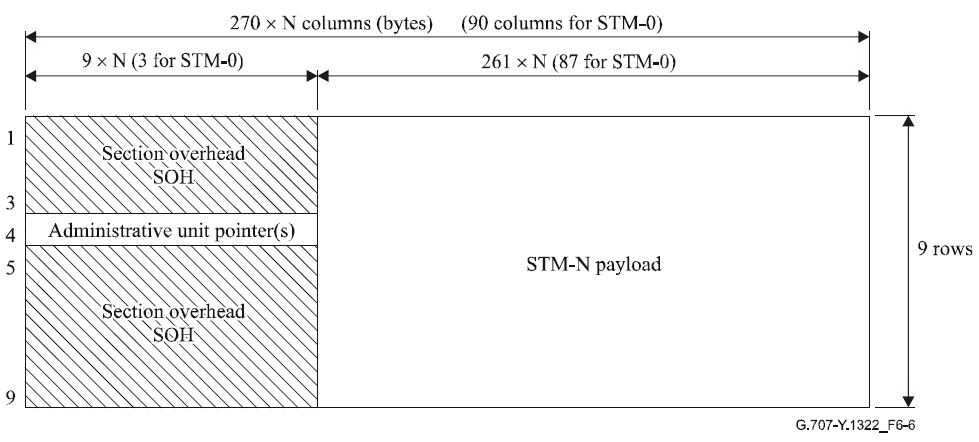
\includegraphics[scale=.6]{FrameSDH.png}
  \caption{Estrutura do \textit{frame} SDH - ITU-T G.707~\cite{G707}.}
 \label{fig:FrameSDH}
\end{figure}

O \textit{frame} SDH � formado por duas principais partes, sendo elas o cabe�alho ou \textit{overhead}, que � composto por 9 x N colunas (sendo N o n�vel da hierarquia) e 9 linhas e o \textit{payload}, composto por 261 x N colunas e 9 linhas. O \textit{payload} � a parte onde os dados dos clientes s�o inseridos para a transmiss�o. O cabe�alho, por sua vez, cont�m as informa��es do quadro \ac{STM}-N referentes a desempenho, manuten��o, monitoramento e indica��es das localidades dos tribut�rios multiplexados nos \textit{frames}, al�m de fun��es operacionais, permitindo uma ger�ncia maior por parte dos n�s da rede. Esta parte do \textit{frame} se subdivide em duas unidades b�sicas, a primeira delas sendo chamada de \ac{SOH} e a segunda de \textit{Administrative Unit Pointers}. � interessante ressaltar que \ac{SOH} ainda � separado em duas partes, sendo elas \ac{RSOH} e \ac{MSOH}, gerando a estrutura ilustrada na Figura~\ref{fig:OverheadSDH} para o cabe�alho. A seguir, apresenta-se uma breve descri��o das funcionalidade contidas em cada uma das partes mencionadas:

\begin{figure}[H]
 \centering
 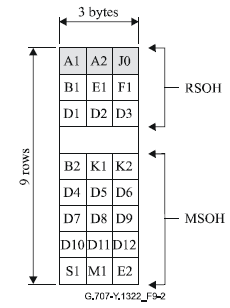
\includegraphics[scale=.7]{OverheadSDH.png}
  \caption{RSOH e MSOH - ITU-T G.707~\cite{G707}.}
 \label{fig:OverheadSDH}
\end{figure}

\begin{itemize}

\item{\bf \ac{SOH}:} Esta se��o se divide em duas partes, como indicado a seguir:

\subitem{\bf \ac{RSOH}:} Parte do cabe�alho que � processada em cada n� destinado a regenera��o. De forma mais espec�fica, essa � uma regi�o do quadro SDH que cont�m informa��es que permitem o alinhamento e identifica��o de \textit{frame}, monitoramento de erro de regenera��o, alarmes f�sicos externos ao equipamento e supervis�o de sistema.
 
\subitem{\bf \ac{MSOH}:} Parte do cabe�alho que � apenas processada em equipamentos onde existe inser��o ou retiradas de canais multiplexados. Inclui informa��es de monitoramento e indica��o de erros de multiplexa��o, controle de chaveamento de mecanismos de prote��o, monitoramento de sincronismo e ger�ncia de sistema.

\item{\bf \textit{Administrative Unit Pointers}:} Esta � uma parte do cabe�alho destinada a prover informa��es de posi��o dos dados dos clientes que foram multiplexados para formarem o \textit{frame} SDH. Possui indica��o de onde se localiza o primeiro \textit{byte} dos \ac{VC} dentro da �rea de informa��o �til (\textit{payload}) e tamb�m pode conter \textit{bytes} provenientes de justifica��o dos \ac{VC}s. � uma parte do cabe�alho processada em cada equipamento da rede

\end{itemize}

\subsection{Camadas de SDH}

A tecnologia SDH apresenta uma estrutura��o em camadas como apresentada na Figura~\ref{fig:SDHlayers}. Atrav�s de tal figura pode ser percebido que SDH possui quatro camadas, sendo elas a Camada de Via (\textit{Path layer}), Camada de Se��o de Multiplexa��o (\textit{Multiplex Section Layer}), Camada de Se��o de Regenera��o (\textit{Regeneration Section Layer}) e Camada F�sica (\textit{Physical Layer}). Para o caso das redes �pticas, a Camada F�sica diz respeito a infraestrutura �ptica de transmiss�o, com seus respectivos dispositivos~\cite{Alwayn2004}.

\begin{figure}[H]
 \centering
 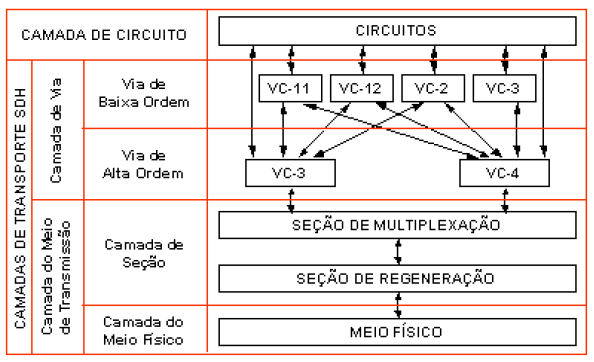
\includegraphics[scale=.7]{SDHlayers.png}
  \caption{Estrutura��o em Camadas de SDH - ~\cite{BernalFilho2003}.}
 \label{fig:SDHlayers}
\end{figure}

O conceito de via em SDH se refere a uma conex�o l�gica entre o ponto em que se monta o quadro SDH padr�o, pela inser��o de tribut�rios e o ponto em que o quadro SDH padr�o � desmontado, pela retirada de tribut�rios, ou seja, se relaciona a uma conex�o l�gica fim-a-fim. A montagem do quadro SDH consiste na a��o de inserir os dados dos clientes nas estruturas denominadas de \textit{Containers}, que consistem em unidades b�sicas de dados com bytes alocados para o transporte dos dados de mais baixas taxas dos clientes, por exemplo pode ser um sinal E1 da hierarquia PDH e associar a esses \textit{Containers} r�tulos denominados de \ac{POH} com informa��es de controle. O processo de desmontagem realiza caminho inverso, retirando o \ac{POH} e o utilizando como informa��o para dar seguimento ao conte�do dos \textit{Containers}. A Camada de Via � justamente respons�vel por realizar tais atividades e est� relacionada � conex�o fim-a-fim entre n�s SDH onde se monta e desmonta o \textit{frame}. � poss�vel que n�s intermedi�rios da rede possam realizar monitoramento de performance dos sinais da Camada de Via, por�m, os bits de cabe�alho referentes a essa camada s�o somente iniciados do ponto de montagem e terminados no ponto de desmontagem do quadro SDH.

O processo descrito anteriormente � indicado na Figura~\ref{fig:SDHlayers}, onde se indica que os dados provenientes da Camada de Circuitos s�o inseridos em \ac{VC}s. E como tamb�m pode ser analisado, a Camada de Via se divide em Via de Baixa Ordem e Via de Alta Ordem. A diferen�a b�sica entre estas duas estruturas consiste no fato de que na Via de Baixa Ordem, dados s�o inseridos em \textit{Containers} de menor tamanho e na Via de Alta Ordem, os \textit{Containers} podem carregar mais de um \ac{VC} anteriormente montado ou carregar dados de clientes que sejam de mais altas taxas de transmiss�o.














\section{OTN}
\label{sec:otn}
ALAELSON
\section{Multiplixa��o}
\label{sec:mux}
subsess�o dentro de cada tecnologia de transporte.

\section{Relacinamento entre Camadas}
\label{sec:layers}
Lailson: Est� � minha parte. Estou modificando via GIT.

\chapter{Plano de Controle}
\label{cap:control}

Alaelson

\section{GMPLS}
\label{sec:gmpls}
Alaelson
\section{SDN}
\label{sec:sdn}
Alaelslon

\chapter{Estudo de Caso: SuperComputing 2014}
\label{cap:case}
falar do chip otn da padtec
Alaelson
\chapter{Conclus�o}
\label{cap:conclusion}

Thyago
\chapter{Tecnologia Transporte}
\label{cap:technology}

\section{Hierarquia Digital Plesi�crona - PDH}
\label{sec:pdh}

Por volta da d�cada de 1970, a infraestrutura de transporte baseava-se na tecnologia \aclu{PDH}. O PDH � um protocolo de comunica��o tradicionalmente desenvolvido para telefonia e que permite o envio de v�rios sinais sobre o mesmo meio, seja cabo coaxial ou fibra �ptica, utilizando t�cnicas de multiplexa��o no tempo e dados em formato digital. O termo \textbf{plesiocr�no} se refere ao fato de que as diferentes termina��es da rede operam com rel�gio quase sincronizados. Como o foco das pesquisas naquele momento estava na comunica��o de voz, demandava-se uma largura de banda de $8~KHz$ para comunica��o bilateral, com 8 bits por amostra que implica na digitaliza��o a uma taxa de $64~Kbps$. Este valor tornou-se padr�o e as transmiss�es de valores superiores foram niveladas em m�ltiplos desse, conforme destacado na Tabela \ref{tab:pdh}, na qual observa-se as taxas padronizadas na hierarquia. Por�m, \ac{PDH} sofria de muitos problemas, o que impulsionou pesquisas de um novo padr�o de multiplexa��o que se consagrou na forma de \ac{SONET} e \ac{SDH}. As principais limita��es do \ac{PDH} s�o:

\begin{itemize}
	\item {\bf Preenchimento de pacotes:} cada terminal opera com um rel�gio individual ligeiramente pr�ximo dos demais e podem ocorrer diferen�as significativas entre dois rel�gios. Assim, antes de realizar a intercala��o � preciso manter os enlaces no mesmo ritmo, o que � feito adicionando bit sem informa��o (bits vazios) que servem para  compensar diferen�as de rel�gio, bits estes descartados na demultiplexa��o.
	\item {\bf Extra��o de n�veis inferiores:} H� uma dificuldade para se extrair um sinal de ordem inferior de um de ordem superior, sem demultiplexar os passos intermedi�rios, ou seja, para extrair o sinal de um enlace em determinado ponto era necess�rio uma demultiplexa��o sucessiva at� o ponto desejado seguida de uma remultiplexa��o para reenvio do sinal.
	\item {\bf Gerenciamento:} falta de informa��es de gerenciamento da rede, monitoramento, identifica��o de conectividade, relat�rio de falhas, al�m de um caminho de comunica��o de dados para transporte dessas informa��es. Isso ocorria devido a limita��o de taxa transportada que n�o permitia aloca��o bits para essas fun��es.
	\item {\bf Compatibilidade:} a falta de descri��o do formato de transmiss�o no meio implicava no desenvolvimento de diferentes formatos de codifica��o e interfaceamento, levando a um problema de incompatibilidade entre equipamentos de diferentes fornecedores.
	\item {\bf Disponibilidade da rede:} o tempo de recupera��o de falhas variava entre segundos at� minutos, valor muito superior aos protocolos sucessores.
\end{itemize}

\begin{table}[!h]
\centering
\caption{Taxas de transmiss�o da tecnologia \ac{PDH} padronizadas na Am�rica do Norte, Europa e Jap�o~\cite{Ramaswami2010}.
\label{tab:pdh}}
\begin{tabular}{c|c|c|c}
\hline
{\bf N�vel} & {\bf Am�rica do Norte} & {\bf Europa} & {\bf Jap�o} \\ \hline
0 & 0.064 Mb/s & 0.064 Mb/s & 0.064 Mb/s \\
1 & 1.544 Mb/s & 2.048 Mb/s & 1.544 Mb/s \\
2 & 6.321 Mb/s & 8.448 Mb/s & 6.321 Mb/s \\
3 & 44.736 Mb/s & 34.368 Mb/s & 32.064 Mb/s \\
4 & 139.264 Mb/s & 139.264 Mb/s & 97.728 Mb/s \\ \hline
\end{tabular}
\end{table}

%\subsection{Multiplexa��o PDH}

O termo multiplexa��o define a tarefa de enviar dois ou mais sinais utilizando o mesmo meio de transmiss�o. Isso pode ser obtido de diversas maneiras, por exemplo, pela divis�o do tempo de acesso ao meio em per�odos de tempos (\textit{time slots}) para cada usu�rio transmitir.

O \ac{PDH} utiliza uma multiplexa��o ass�ncrona, na qual cada terminal tem seu pr�prio \textit{clock}, levando a imprecis�es entre as suas taxas de funcionamento, mesmo quando adotada um \textit{clock} nominal. Assim, para que haja corre��o nessas pequenas diferen�as, deve ser inserir bits nos fluxos. Para que seja poss�vel se captar um fluxo mais lento de informa��o multiplexado num fluxo mais r�pido, � necess�rio uma estrutura chamada ``montanha de multiplexadores'' (ver Figura~\ref{fig:muxPDH}), o que elevava o custo e complexidade das redes. 

\begin{figure}[!htb]
\centering
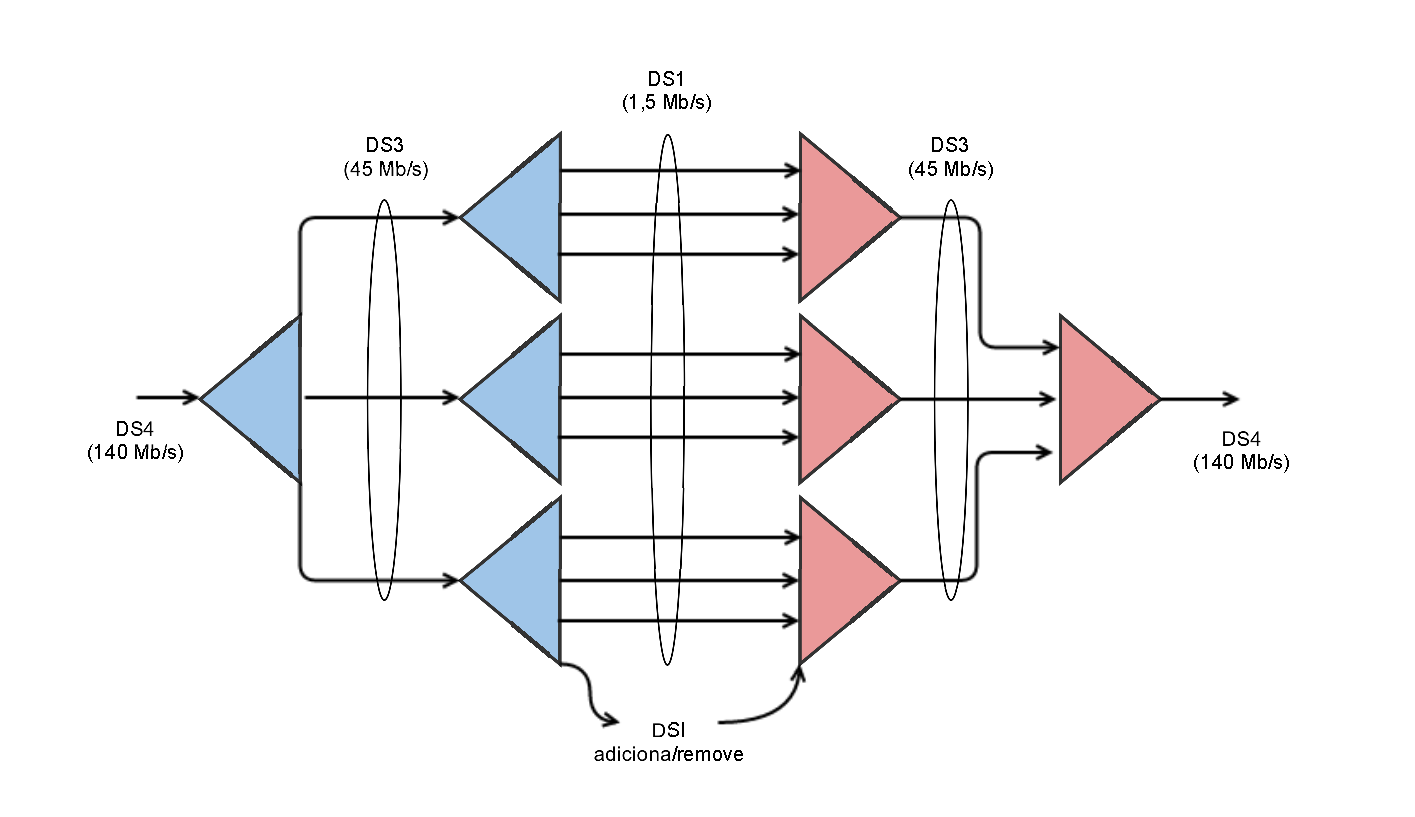
\includegraphics[width=.7\textwidth]{image/mux_pdh.eps}
\caption{\label{fig:muxPDH} Estrutura de multiplexa��o PDH: a ``montanha de multiplexadores''. Adaptado de \cite{Ramaswami2010}.}
\end{figure}

\section{SONET/SDH}
\label{sec:sdh}
%
A tecnologia de transporte PDH, que foi introduzida para atender a demanda de multiplexa��o de canais de voz, apresentava uma s�rie de limita��es tecnol�gicas e operacionais, o que fez com que na d�cada de 1980 fornecedores de servi�os de telecomunica��es e fabricantes de equipamentos buscassem novos padr�es de transmiss�o e multiplexa��o, com foco na transmiss�o �ptica. Em 1984, a associa��o americana chamada \ac{ECSA} iniciou trabalhos com a finalidade de desenvolvimento de um padr�o que atendesse as necessidades das telecomunica��es essencialmente nos Estados Unidos, propondo-o ao \ac{ANSI} e no ano de 1985, j� se tinham resultados que conduziram ao in�cio da padroniza��o da tecnologia de transporte em redes de telecomunica��es chamada de \ac{SONET}~\cite{Ballart2002}, adotado em pa�ses como Estados Unidos, Canada e Jap�o. O  \ac{CCITT}, atualmente conhecido como \ac{ITU-T}, demonstrou interesse pelo padr�o \ac{ANSI}~\cite{Boehm1990} e prop�s mudan�as para a acomoda��o de ambas as hierarquias de taxas de transmiss�o americanas e europeias e finalmente em 1988 alcan�ou-se um acordo, de modo que o �rg�o CCITT definiu o padr�o conhecido como \ac{SDH}, amplamente adotado na Europa e tamb�m no Brasil. As recomenda��es ANSI T1.105, ANSI T1.106 e ANSI T1.117 s�o exemplos de publica��es que definem par�metros relacionados a SONET enquanto as recomenda��es ITU-T G.691, ITU-T G.707 e ITU-T G.781 s�o exemplos relacionados ao padr�o SDH.

SONET e SDH guardam os mesmos conceitos tecnol�gicos e as principais diferen�as se situam em certas denomina��es de par�metros e nas taxas de transmiss�o definidas nas hierarquias. Esses dois padr�es foram desenvolvidos visando a comunica��o por meio de fibras �pticas mas, por exemplo, SDH foi tamb�m utilizado em sistemas baseados em radio-frequ�ncia. Comparando estes dois padr�es com a tecnologia PDH, podem ser destacados as seguintes vantagens:

\begin{itemize}

\item {\bf Simplifica��es no processo de multiplexa��o:} Como j� visto anteriormente, o processo de retirada de sinais tribut�rios de baixas taxas de um sinal multiplexado de taxa superior � uma opera��o dif�cil na tecnologia PDH, devido ao fato de que s�o necess�rias demultiplexa��es e multiplexa��es sucessivas para se poder localizar o tribut�rio requerido, retir�-lo e ent�o remontar o frame de alta taxa. Isso acaba implicando em altos custos de instala��o da rede PDH e em baixa confiabilidade devido a quantidade de dispositivos eletr�nicos envolvidos nos n�s aos longo da rede. A estrutura de multiplexa��o s�ncrona de SONET/SDH permite significativa redu��o de complexidade e custos relacionados ao processo de extra��o e inser��o de tribut�rios em sinais multiplexados bem como aumenta a confiabilidade do sistema como um todo. Isso porque nas redes SONET/SDH, todos os n�s da rede tem clock sincronizados, de modo que as taxas de transmiss�o s�o simplesmente m�ltiplos de um valor base e n�o se � necess�rio o preenchimento de um tribut�rio com bits vazios para possibilitar a multiplexa��o, como era necess�rio na tecnologia PDH. Assim, a extra��o de um sinal tribut�rio de um sinal de alta taxa � simplificada. Esse processo � ainda mais simplificado devido a utiliza��o de um \textit{frame} que permite serem inseridas maiores informa��es sobre o \textit{payload}. O processo de inser��o de tribut�rios tamb�m se torna simplificado, j� que os sinais possuem taxas de transmiss�o muito mais precisas e pr�ximas umas das outras do que na tecnologia PDH~\cite{Ramaswami2010}.

\item{\bf Informa��es de Gerenciamento:} Os padr�es SONET e SDH oferecem maiores recursos de monitoramento, gerenciamento e controle do que est� presente nas redes PDH. Como ser� visto mais adiante, o \textit{frame} dos padr�es SONET e SDH oferecem campos espec�ficos a atividade de monitoramento e gest�o da comunica��o.

\item{\bf Interoperabilidade:} � dif�cil tratar de conceitos de telecomunica��es sem levar em considera��o um dos princ�pios b�sicos dessa �rea que � a Interoperabilidade. Anteriormente foi mencionado que isto era um problema nos sistemas PDH, pois diferentes fornecedores de equipamentos utilizavam interfaces e codifica��es distintas, dificultando a compatibilidade ao longo da rede. SONET e SDH s�o padr�es que tentam eliminar este problema por meio da defini��o de par�metros padr�es, como as interfaces.

\item{\bf Disponibilidade da rede:} SONET e SDH s�o padr�es que evolu�ram para acomodar espec�ficas topologias de rede e t�cnicas de prote��o e protocolos associados para possibilitar altos n�veis de disponibilidade. Como consequ�ncia, a atua��o da prote��o � em geral mais r�pida do que nas redes PDH. 


\end{itemize} 

A seguir, ser�o abordadas caracter�sticas importantes referentes a SDH. Por�m, os conceitos tamb�m se aplicam ao padr�o SONET, visto que SDH foi desenvolvido a partir do mesmo.

\subsection{Estrutura do \textit{frame} SDH}

Uma das principais caracter�sticas do \textit{frame} SDH � sua bidimensionalidade, j� que tal \textit{frame} � definido por uma quantidade de linhas e colunas como ilustrado na Figura~\ref{fig:FrameSDH}. O \textit{frame} SDH possui um n�mero fixo de linhas e um n�mero de colunas dependente da hierarquia SDH a que se est� referenciando. De forma mais precisa, tal \textit{frame} possui 9 linhas e 270 x N colunas, onde N � o termo dependente da hierarquia e que pode ser obtido observando que as hierarquias s�o definidas seguindo o padr�o \ac{STM}-N, para N igual a 1, 4, 16, 64 e 256 e � interessante ressaltar que para o caso STM-0 existem apenas 9 linhas e 90 colunas como j� indicado na Figura~\ref{fig:FrameSDH}, correspondendo ao \textit{frame} STS-1 do padr�o SONET. Cada linha nesta estrutura � tratada como um \textit{bit} enquanto cada coluna � tratada como um \textit{byte}. Outra caracter�stica importante � que independentemente do tamanho e consequentemente do n�mero de bits do \textit{frame}, sua dura��o � sempre de 125 \(\mu s\), representando uma taxa de repeti��o de 8000 kHz herdada dos antigos sistemas PDH. Nessa estrutura, os bits s�o transmitidos, da esquerda para a direita, em cada linha at� se alcan�ar o fim do \textit{frame}.

\begin{figure}[H]
 \centering
 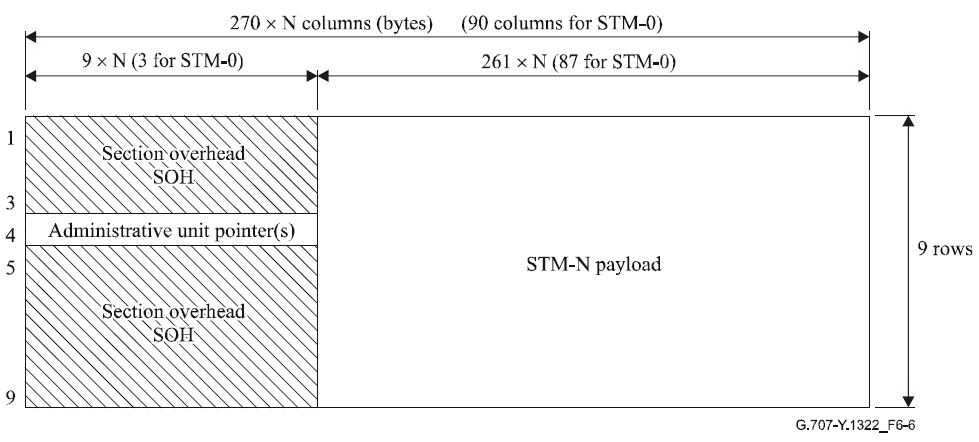
\includegraphics[scale=.6]{FrameSDH.png}
  \caption{Estrutura do \textit{frame} SDH - ITU-T G.707~\cite{G707}.}
 \label{fig:FrameSDH}
\end{figure}

O \textit{frame} SDH � formado por duas principais partes, sendo elas o cabe�alho ou \textit{overhead}, que � composto por 9 x N colunas (sendo N o n�vel da hierarquia) e 9 linhas e o \textit{payload}, composto por 261 x N colunas e 9 linhas. O \textit{payload} � a parte onde os dados dos clientes s�o inseridos para a transmiss�o. O cabe�alho, por sua vez, cont�m as informa��es do quadro \ac{STM}-N referentes a desempenho, manuten��o, monitoramento e indica��es das localidades dos tribut�rios multiplexados nos \textit{frames}, al�m de fun��es operacionais, permitindo uma ger�ncia maior por parte dos n�s da rede. Esta parte do \textit{frame} se subdivide em duas unidades b�sicas, a primeira delas sendo chamada de \ac{SOH} e a segunda de \textit{Administrative Unit Pointers}. � interessante ressaltar que \ac{SOH} ainda � separado em duas partes, sendo elas \ac{RSOH} e \ac{MSOH}, gerando a estrutura ilustrada na Figura~\ref{fig:OverheadSDH} para o cabe�alho. A seguir, apresenta-se uma breve descri��o das funcionalidade contidas em cada uma das partes mencionadas:

\begin{figure}[H]
 \centering
 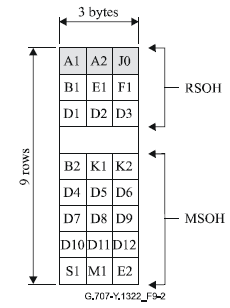
\includegraphics[scale=.7]{OverheadSDH.png}
  \caption{RSOH e MSOH - ITU-T G.707~\cite{G707}.}
 \label{fig:OverheadSDH}
\end{figure}

\begin{itemize}

\item{\bf \ac{SOH}:} Esta se��o se divide em duas partes, como indicado a seguir:

\subitem{\bf \ac{RSOH}:} Parte do cabe�alho que � processada em cada n� destinado a regenera��o. De forma mais espec�fica, essa � uma regi�o do quadro SDH que cont�m informa��es que permitem o alinhamento e identifica��o de \textit{frame}, monitoramento de erro de regenera��o, alarmes f�sicos externos ao equipamento e supervis�o de sistema.
 
\subitem{\bf \ac{MSOH}:} Parte do cabe�alho que � apenas processada em equipamentos onde existe inser��o ou retiradas de canais multiplexados. Inclui informa��es de monitoramento e indica��o de erros de multiplexa��o, controle de chaveamento de mecanismos de prote��o, monitoramento de sincronismo e ger�ncia de sistema.

\item{\bf \textit{Administrative Unit Pointers}:} Esta � uma parte do cabe�alho destinada a prover informa��es de posi��o dos dados dos clientes que foram multiplexados para formarem o \textit{frame} SDH. Possui indica��o de onde se localiza o primeiro \textit{byte} dos \ac{VC} dentro da �rea de informa��o �til (\textit{payload}) e tamb�m pode conter \textit{bytes} provenientes de justifica��o dos \ac{VC}s. � uma parte do cabe�alho processada em cada equipamento da rede

\end{itemize}

\subsection{Camadas de SDH}

A tecnologia SDH apresenta uma estrutura��o em camadas como apresentada na Figura~\ref{fig:SDHlayers}. Atrav�s de tal figura pode ser percebido que SDH possui quatro camadas, sendo elas a Camada de Via (\textit{Path layer}), Camada de Se��o de Multiplexa��o (\textit{Multiplex Section Layer}), Camada de Se��o de Regenera��o (\textit{Regeneration Section Layer}) e Camada F�sica (\textit{Physical Layer}). Para o caso das redes �pticas, a Camada F�sica diz respeito a infraestrutura �ptica de transmiss�o, com seus respectivos dispositivos~\cite{Alwayn2004}.

\begin{figure}[H]
 \centering
 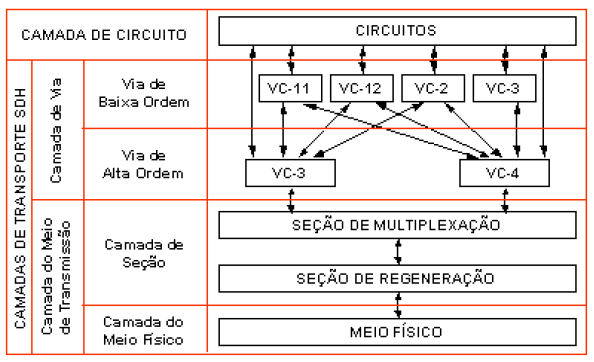
\includegraphics[scale=.7]{SDHlayers.png}
  \caption{Estrutura��o em Camadas de SDH - ~\cite{BernalFilho2003}.}
 \label{fig:SDHlayers}
\end{figure}

O conceito de via em SDH se refere a uma conex�o l�gica entre o ponto em que se monta o quadro SDH padr�o, pela inser��o de tribut�rios e o ponto em que o quadro SDH padr�o � desmontado, pela retirada de tribut�rios, ou seja, se relaciona a uma conex�o l�gica fim-a-fim. A montagem do quadro SDH consiste na a��o de inserir os dados dos clientes nas estruturas denominadas de \textit{Containers}, que consistem em unidades b�sicas de dados com bytes alocados para o transporte dos dados de mais baixas taxas dos clientes, por exemplo pode ser um sinal E1 da hierarquia PDH e associar a esses \textit{Containers} r�tulos denominados de \ac{POH} com informa��es de controle. O processo de desmontagem realiza caminho inverso, retirando o \ac{POH} e o utilizando como informa��o para dar seguimento ao conte�do dos \textit{Containers}. A Camada de Via � justamente respons�vel por realizar tais atividades e est� relacionada � conex�o fim-a-fim entre n�s SDH onde se monta e desmonta o \textit{frame}. � poss�vel que n�s intermedi�rios da rede possam realizar monitoramento de performance dos sinais da Camada de Via, por�m, os bits de cabe�alho referentes a essa camada s�o somente iniciados do ponto de montagem e terminados no ponto de desmontagem do quadro SDH.

O processo descrito anteriormente � indicado na Figura~\ref{fig:SDHlayers}, onde se indica que os dados provenientes da Camada de Circuitos s�o inseridos em \ac{VC}s. E como tamb�m pode ser analisado, a Camada de Via se divide em Via de Baixa Ordem e Via de Alta Ordem. A diferen�a b�sica entre estas duas estruturas consiste no fato de que na Via de Baixa Ordem, dados s�o inseridos em \textit{Containers} de menor tamanho e na Via de Alta Ordem, os \textit{Containers} podem carregar mais de um \ac{VC} anteriormente montado ou carregar dados de clientes que sejam de mais altas taxas de transmiss�o.














A tecnologia de transporte PDH, que foi introduzida para atender a demanda de multiplexa��o de canais de voz, apresentava uma s�rie de limita��es tecnol�gicas e operacionais, o que fez com que na d�cada de 1980 fornecedores de servi�os de telecomunica��es e fabricantes de equipamentos buscassem novos padr�es de transmiss�o e multiplexa��o, com foco na transmiss�o �tica. Em 1984, a associa��o americana chamada \ac{ECSA} iniciou trabalhos com a finalidade de desenvolvimento de um padr�o que atendesse as necessidades das telecomunica��es essencialmente nos Estados Unidos, propondo-o ao \ac{ANSI} e no ano de 1985, j� se tinham resultados que conduziram ao in�cio da padroniza��o da tecnologia de transporte em redes de telecomunica��es chamada de \ac{SONET}~\cite{Ballart2002}, adotado em pa�ses como Estados Unidos, Canada e Jap�o. O  \ac{CCITT}, atualmente conhecido como \ac{ITU-T}, demonstrou interesse pelo padr�o \ac{ANSI}~\cite{Boehm1990} e prop�s mudan�as para a acomoda��o de ambas as hierarquias de taxas de transmiss�o americanas e europeias e finalmente em 1988 alcan�ou-se um acordo, de modo que o �rg�o CCITT definiu o padr�o conhecido como \ac{SDH}, amplamente adotado na Europa e tamb�m no Brasil. As recomenda��es ANSI T1.105, ANSI T1.106 e ANSI T1.117~\cite{Zhang2001} definem o padr�o SONET, enquanto as recomenda��es ITU-T G.691~\cite{G691.1}, ITU-T G.707~\cite{G707} e ITU-T G.781~\cite{G781} padronizam o SDH. 

SONET e SDH guardam os mesmos conceitos tecnol�gicos e as principais diferen�as se situam em certas denomina��es de par�metros e nas taxas de transmiss�o definidas nas hierarquias. Esses dois padr�es foram desenvolvidos visando a comunica��o por meio de fibras �ticas mas, por exemplo, SDH foi tamb�m utilizado em sistemas baseados em radio-frequ�ncia. Comparando estes dois padr�es com a tecnologia PDH, podem ser destacados as seguintes vantagens:

\begin{itemize}

%Como j� visto anteriormente, o processo de retirada de sinais tribut�rios de baixas taxas de um sinal multiplexado de taxa superior � uma opera��o dif�cil na tecnologia PDH, devido ao fato de que s�o necess�rias demultiplexa��es e multiplexa��es sucessivas para se poder localizar o tribut�rio requerido, retir�-lo e ent�o remontar o frame de alta taxa. Isso acaba implicando em altos custos de instala��o da rede PDH e em baixa confiabilidade devido a quantidade de dispositivos eletr�nicos envolvidos nos n�s aos longo da rede.

\item {\bf multiplexa��o simplificada:} A estrutura de multiplexa��o s�ncrona permite significativa redu��o de complexidade e custos relacionados ao processo de extra��o e inser��o de tribut�rios, bem como, aumenta a confiabilidade do sistema como um todo, devido ao \textit{clock} sincronizado de todos os n�s da rede. As taxas de transmiss�o s�o simplesmente m�ltiplos de um valor base e n�o sendo necess�rio o preenchimento de um tribut�rio com bits vazios para possibilitar a multiplexa��o, como era necess�rio na tecnologia PDH. Assim, a extra��o de um sinal tribut�rio de a partir de outro de taxa mais alta � facilitado. Esse processo � ainda mais simples devido a utiliza��o de um \textit{frame} que permite serem inseridas maiores informa��es sobre a carga �til (\textit{payload}). O processo de inser��o de tribut�rios tamb�m � simples, j� que os sinais possuem taxas de transmiss�o muito mais precisas e pr�ximas umas das outras~\cite{Ramaswami2010}.

\item{\bf Informa��es de Gerenciamento:} novos recursos de monitoramento, gerenciamento e controle foram incorporados no \textit{frame}.

\item{\bf Interoperabilidade:} interfaces e par�metros padronizados foram definidos para que haja interoperabilidade entre equipamentos de diferentes fabricantes.

%� dif�cil tratar de conceitos de telecomunica��es sem levar em considera��o um dos princ�pios b�sicos dessa �rea que � a Interoperabilidade. Anteriormente foi mencionado que isto era um problema nos sistemas PDH, pois diferentes fornecedores de equipamentos utilizavam interfaces e codifica��es distintas, dificultando a compatibilidade ao longo da rede. SONET e SDH s�o padr�es que tentam eliminar este problema por meio da defini��o de par�metros padr�es, como as interfaces.

\item{\bf Disponibilidade da rede:} Novas t�cnicas de recupera��o e prote��o foram especificadas para topologias de rede em Anel. As t�cnicas de prote��o e protocolos associados para possibilitar altos n�veis de disponibilidade s�o em geral s�o mais r�pidas do que nas redes PDH.


\end{itemize} 

%A seguir, ser�o abordadas caracter�sticas importantes referentes a SDH. Por�m, os conceitos tamb�m se aplicam ao padr�o SONET, visto que SDH foi desenvolvido a partir do mesmo.

\subsection{Multiplexa��o SONET}
\label{subsec:mux_sonet}

Os m�todos de multiplexa��o nas tecnologias SONET e SDH s�o bastante sofisticados e podem ser implementados em circuitos integrados de longa escala. Comparando a Figura \ref{fig:muxSDH} com a Figura \ref{fig:muxPDH}, � poss�vel notar que somente um componente � necess�rio para fazer o que a ``montanha de multiplexadores'' utilizando-se SONET/SDH, o que reduz bastante a complexidade em rela��o � multiplexa��o PDH.

Para SONET a taxa de sinal b�sica � $51,84 \, Mb/s$, chamada de \aclu{STS} \textit{level}-1 (STS-1). As outras taxas derivadas desta s�o chamadas STS-N e s�o obtidas alternando os \textit{bytes} de N \textit{frames} STS-1 alinhados. Como os \textit{clocks} dos sinais s�o sincronizados, n�o h� necessidade de inser��o de bits. Por esse mesmo motivo, sinais de taxas menores podem ser extra�dos de um fluxo multiplexado sem necessidade de demultiplexar o sinal inteiro. A tabela \ref{tab:taxasSONET} traz as taxas de transmiss�o e nomenclatura SONET.

\begin{figure}[!htb]
\centering
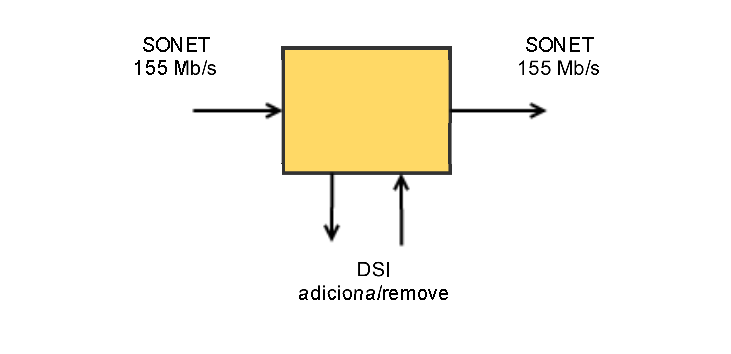
\includegraphics[width=0.5\textwidth]{image/mux_sonet.eps}
\caption{\label{fig:muxSDH} Estrutura de multiplexa��o SONET. Adaptado de \cite{Ramaswami2010}.}
\end{figure}

\begin{table}[!htb]
\centering
\caption{Nomenclaturas de interfaces e taxas de transmiss�o da tecnologia SONET. Adaptado de \cite{Ramaswami2010}.}
\label{tab:taxasSONET}
\begin{tabular}{c|c}
\hline
Nomenclatura & Taxa de Bit (Mb/s) \\\hline
STS-1 & $51,84$ \\
STS-3 & $155,52$ \\
STS-12 & $622,08$ \\
STS-24 & $1244,16$ \\
STS-48 & $2488,32$ \\
STS-192 & $9953,28$ \\
STS-768 & $39.814,32$ \\\hline
\end{tabular}
\end{table}

Em SONET, os fluxos de dados de taxa inferior a STS-1 s�o mapeados em \textit{Virtual Tributaries} (VTs). Os VTs s�o divididos em quatro tamanhos: VT1.5, VT2, VT3 e VT6, que acomodam fluxos ass�ncronos e plesi�cronos de $1,5$, $2$, $3$ e $6 \, Mb/s$, respectivamente. Esses VTs s�o agrupados em um grupo VT que podem ter quatro VT1.5, tr�s VT2, dois VT3 ou um �nico VT6. Cada grupo �, ent�o, intercalado \textit{byte}-a-\textit{byte} junto com um junto de \textit{overheads} de caminho para formar o SONET SPE (\textit{synchronous payload envelope}) b�sico. A figura \ref{fig:vt} mostra graficamente como funciona a hierarquia SONET. 

Para camadas clientes (de maior abstra��o), como IP ou Ethernet, que tem tamanho de pacotes grandes, � usada a nomenclatura STS-Nc, em que o "c" denomina "concatenado". 

\begin{figure}[!htb]
\centering
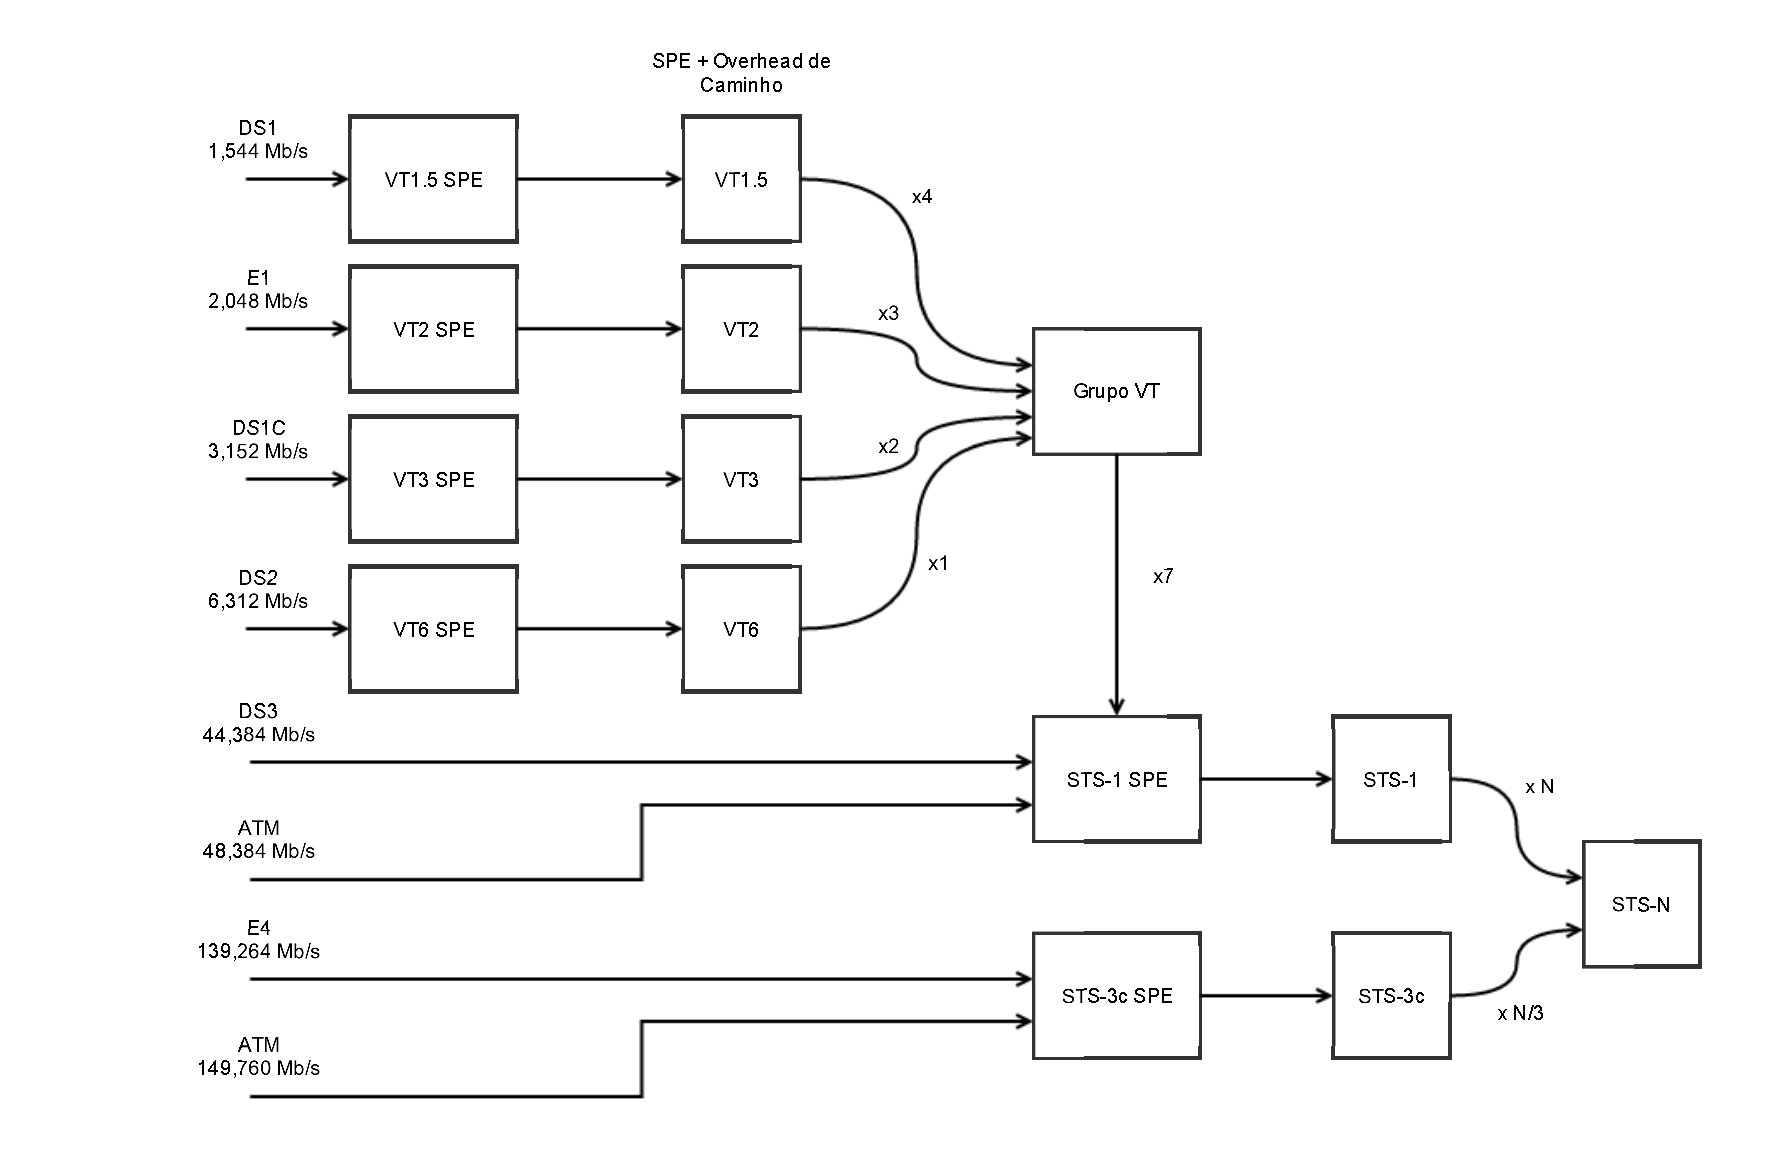
\includegraphics[width=1\textwidth]{image/vt.eps}
\caption{Esquema de multiplexa��o utilizando \textit{Virtual Tributaries} em SONET. Adaptado de \cite{Ramaswami2010}}
\label{fig:vt}.
\end{figure}

\subsection{Multiplexa��o SDH}
\label{subsec:mux_sdh}

Para SDH, a taxa b�sica � $155 \, Mb/s$ e � chamada STM-1 (\textit{synchronous transport module-1}). Que foi escolhido para acomodar as taxas PDH mais utilizadas (DS1 e DS3). A tabela \ref{tab:taxasSDH} mostra as taxas de transmiss�o definidas para SDH.

\begin{table}[!htb]
\centering
\caption{Nomenclaturas de interfaces e taxas de transmiss�o da tecnologia SDH.}
\label{tab:taxasSDH} 
\begin{tabular}{c|c} \hline
SDH & Taxa de Bit (Mb/s) \\\hline
STM-1 & $155,52$ \\
STM-4 & $622,08$ \\
STM-16 & $2488,32$ \\
STM-64 & $9953,28$ \\
STM-256 & $39814,32$ \\\hline
\end{tabular}
\end{table}

Em SDH, os \textit{Virtual Containers} (VCs) fazem o mesmo trabalho dos VTs em SONET. Os VCs tem quatro tamanhos: VC-11, VC-12, VC-2, VC-3 e VC-4, que carregam fluxos de $1,5$, $2$, $6$, $45$ e $140 \, Mb/s$. Diferentemente de SONET, em SDH tem-se uma hierarquia em dois est�gios em que VC-11, VC-12 e VC-2 podem ser multiplexados em VC-3 e VC-3 e VC-4 podem ser multiplexados em sinais STM-1.

\subsection{Estrutura do \textit{frame} SDH}
\label{subsec:frame_sdh}

Uma das principais caracter�sticas do \textit{frame} SDH � sua bidimensionalidade, j� que tal \textit{frame} � definido por uma quantidade de linhas e colunas como ilustrado na Figura~\ref{fig:FrameSDH}. O \textit{frame} SDH possui um n�mero fixo de linhas e um n�mero de colunas dependente da hierarquia SDH a que se est� referenciando. De forma mais precisa, tal \textit{frame} possui 9 linhas e 270 x N colunas, onde N � o termo dependente da hierarquia e que pode ser obtido observando que as hierarquias s�o definidas seguindo o padr�o \ac{STM}-N, para N igual a 1, 4, 16, 64 e 256 e � interessante ressaltar que para o caso STM-0 existem apenas 9 linhas e 90 colunas como j� indicado na Figura~\ref{fig:FrameSDH}, correspondendo ao \textit{frame} STS-1 do padr�o SONET. Cada linha nesta estrutura � tratada como um \textit{bit} enquanto cada coluna � tratada como um \textit{byte}. Outra caracter�stica importante � que independentemente do tamanho e consequentemente do n�mero de bits do \textit{frame}, sua dura��o � sempre de 125 \(\mu s\), representando uma taxa de repeti��o de 8000 kHz herdada dos antigos sistemas PDH. Nessa estrutura, os bits s�o transmitidos, da esquerda para a direita, em cada linha at� se alcan�ar o fim do \textit{frame}.

\begin{figure}[!htb]
 \centering
 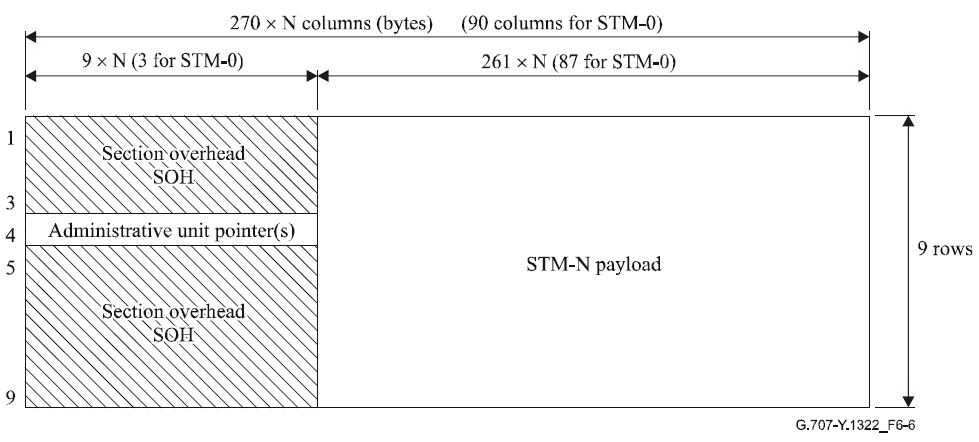
\includegraphics[scale=.6]{FrameSDH.png}
  \caption{Estrutura do \textit{frame} SDH - ITU-T G.707~\cite{G707}.}
 \label{fig:FrameSDH}
\end{figure}

O \textit{frame} SDH � formado por duas principais partes, sendo elas o cabe�alho ou \textit{overhead}, que � composto por 9 x N colunas (sendo N o n�vel da hierarquia) e 9 linhas e o \textit{payload}, composto por 261 x N colunas e 9 linhas. O \textit{payload} � a parte onde os dados dos clientes s�o inseridos para a transmiss�o. O cabe�alho, por sua vez, cont�m as informa��es do quadro \ac{STM}-N referentes a desempenho, manuten��o, monitoramento e indica��es das localidades dos tribut�rios multiplexados nos \textit{frames}, al�m de fun��es operacionais, permitindo uma ger�ncia maior por parte dos n�s da rede. Esta parte do \textit{frame} se subdivide em duas unidades b�sicas, a primeira delas sendo chamada de \ac{SOH} e a segunda de \textit{Administrative Unit Pointers}. � interessante ressaltar que \ac{SOH} ainda � separado em duas partes, sendo elas \ac{RSOH} e \ac{MSOH}, gerando a estrutura ilustrada na Figura~\ref{fig:OverheadSDH} para o cabe�alho. A seguir, apresenta-se uma breve descri��o das funcionalidade contidas em cada uma das partes mencionadas:

\begin{figure}[!htb]
 \centering
 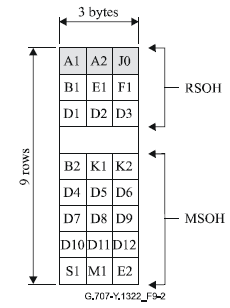
\includegraphics[scale=.7]{OverheadSDH.png}
  \caption{RSOH e MSOH - ITU-T G.707~\cite{G707}.}
 \label{fig:OverheadSDH}
\end{figure}

\begin{itemize}

\item{\bf \ac{SOH}:} Esta se��o se divide em duas partes, como indicado a seguir:

\subitem{\bf \ac{RSOH}:} Parte do cabe�alho que � processada em cada n� destinado a regenera��o. De forma mais espec�fica, essa � uma regi�o do quadro SDH que cont�m informa��es que permitem o alinhamento e identifica��o de \textit{frame}, monitoramento de erro de regenera��o, alarmes f�sicos externos ao equipamento e supervis�o de sistema.
 
\subitem{\bf \ac{MSOH}:} Parte do cabe�alho que � apenas processada em equipamentos onde existe inser��o ou retiradas de canais multiplexados. Inclui informa��es de monitoramento e indica��o de erros de multiplexa��o, controle de chaveamento de mecanismos de prote��o, monitoramento de sincronismo e ger�ncia de sistema.

\item{\bf \textit{Administrative Unit Pointers}:} Esta � uma parte do cabe�alho destinada a prover informa��es de posi��o dos dados dos clientes que foram multiplexados para formarem o \textit{frame} SDH. Possui indica��o de onde se localiza o primeiro \textit{byte} dos \ac{VC} dentro da �rea de informa��o �til (\textit{payload}) e tamb�m pode conter \textit{bytes} provenientes de justifica��o dos \ac{VC}s. � uma parte do cabe�alho processada em cada equipamento da rede

\end{itemize}

\subsection{Camadas do padr�o SDH}

A tecnologia SDH apresenta uma estrutura��o em camadas como apresentada na Figura~\ref{fig:SDHlayers}. Atrav�s de tal figura pode ser percebido que SDH possui quatro camadas, sendo elas a Camada de Via (\textit{Path layer}), Camada de Se��o de Multiplexa��o (\textit{Multiplex Section Layer}), Camada de Se��o de Regenera��o (\textit{Regeneration Section Layer}) e Camada F�sica (\textit{Physical Layer}). Com exce��o da Camada F�sica, as camadas possuem um conjunto de \textit{bytes} no \textit{Overhead} a que s�o relacionados e que s�o utilizadas para a realiza��o de diversas funcionalidades, como avalia��o de desempenho~\cite{Alwayn2004}.

O conceito de via em SDH se refere a uma conex�o l�gica entre o ponto em que se monta o quadro SDH padr�o, pela inser��o de tribut�rios e o ponto em que o quadro SDH padr�o � desmontado, pela retirada de tribut�rios, ou seja, se relaciona a uma conex�o l�gica fim-a-fim. A montagem do quadro SDH consiste na a��o de inserir os dados dos clientes nas estruturas denominadas de \textit{Containers}, que consistem em unidades b�sicas de dados com bytes alocados para o transporte dos dados de mais baixas taxas dos clientes, por exemplo pode ser um sinal E1 da hierarquia PDH e associar a esses \textit{Containers} r�tulos denominados de \ac{POH} com informa��es de controle. O processo de desmontagem realiza caminho inverso, retirando o \ac{POH} e o utilizando como informa��o para dar seguimento ao conte�do dos \textit{Containers}. A Camada de Via � justamente respons�vel por realizar tais atividades e est� relacionada � conex�o fim-a-fim entre n�s SDH onde se monta e desmonta o \textit{frame}. � poss�vel que n�s intermedi�rios da rede possam realizar monitoramento de performance dos sinais da Camada de Via, por�m, os \textit{bytes} de cabe�alho referentes a essa camada s�o somente iniciados do ponto de montagem e terminados no ponto de desmontagem do quadro SDH, por exemplo, nos \ac{TM}

\begin{figure}[!htb]
 \centering
 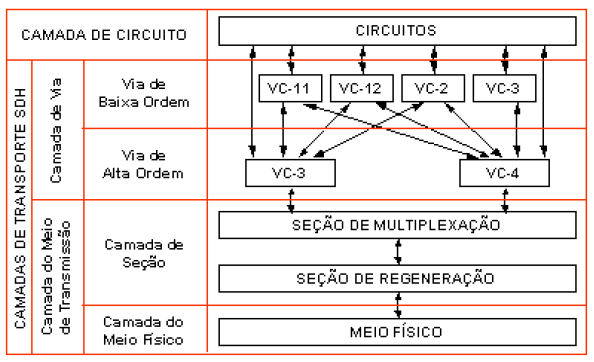
\includegraphics[scale=.7]{SDHlayers.png}
  \caption{Estrutura��o em Camadas do padr�o SDH - ~\cite{BernalFilho2003}.}
 \label{fig:SDHlayers}
\end{figure}

O processo descrito anteriormente � indicado na Figura~\ref{fig:SDHlayers}, onde se indica que os dados provenientes da Camada de Circuitos s�o inseridos em \ac{VC}s. E como tamb�m pode ser analisado, a Camada de Via se divide em Via de Baixa Ordem e Via de Alta Ordem. A diferen�a b�sica entre estas duas estruturas consiste no fato de que na Via de Baixa Ordem, dados s�o inseridos em \textit{Containers} de menor tamanho e na Via de Alta Ordem, os \textit{Containers} podem carregar mais de um \ac{VC} anteriormente montado ou carregar dados de clientes que sejam de mais altas taxas de transmiss�o.

A Camada de Se��o de Multiplexa��o � respons�vel por multiplexar um n�mero de conex�es da Camada de Via em um �nico link (meio de transmiss�o) entre dois n�s. Assim, os \textit{bytes} de cabe�alho referentes a essa camada s�o acessados e processados em cada elemento da conex�o respons�vel por realizar multiplexa��o. Por exemplo, a camada em quest�o � acessada nos \ac{TM}s e nos \ac{ADM}s.

Por sua vez, a Camada de Se��o de Regenera��o � utilizada entre elementos adjacentes de um link \ac{SDH}, ou seja, ela � utilizada para o processamento dos \textit{frames} em todos os equipamentos da rede, sejam eles de passagem, extra��o ou inser��o dos tribut�rios~\cite{BernalFilho2003}. A Figura~\ref{fig:SDHlayersConection} apresenta a rela��o das camadas e dos diversos dispositivos presentes em uma rede, assim como descrito anteriormente. Esta Figura utiliza a mesma nomenclatura anteriormente descrita e insere um dispositivo espec�fico de regenera��o do \textit{frame}, referenciado na Figura~\ref{fig:SDHlayersConection} como \ac{REG}. 

\begin{figure}[!htb]
 \centering
 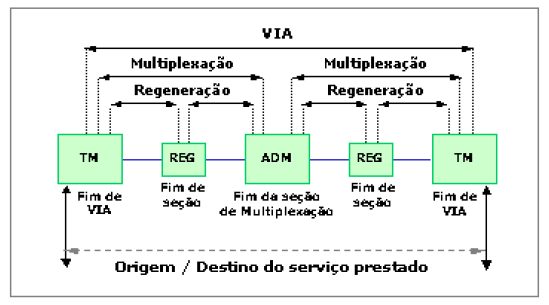
\includegraphics[scale=.7]{SDHlayersConection.png}
  \caption{Relacionamento Longitudinal entre as Camadas nos Elementos de Rede~\cite{BernalFilho2003}.}
 \label{fig:SDHlayersConection}
\end{figure} 

A Camada F�sica diz respeito a infraestrutura de conex�es que permite a transmiss�o dos \textit{frames}. Para o caso das Comunica��es �pticas, a Camada F�sica engloba todos os dispositivos �pticos envolvidos na transmiss�o na fibra �ptica, como por exemplo \textit{lasers} e fotodetectores. � interessante ressaltar que o processamento dos \textit{frames} \ac{SDH} ocorre no dom�nio el�trico e por isso, esta camada tamb�m � respons�vel por adequar a transmiss�o dos \textit{frames} que originalmente est�o no dom�nio el�trico atrav�s do meio de transmiss�o que se est� utilizando. Continuando o exemplo relacionado as Comunica��es �pticas, a Camada F�sica define interfaces que permitem realizar a transmiss�o e recep��o atrav�s das fibras �pticas com a utiliza��o de dispositivos �pticos como \textit{lasers} e fotodetectores. O \ac{ITU-T} define interfaces f�sicas para a transmiss�o sobre fibras �pticas para SDH nas recomenda��es G.957 e G.691. Como exemplo, a Figura~\ref{fig:PhysicalSDH} ilustra estas interfaces, definindo os tipos de fibras, atenua��es e dispers�es aceit�veis do enlace e tipos de transmissores com rela��o ao comprimento de onda de opera��o, taxa de transmiss�o e comprimento do enlace.

\begin{figure}[!htb]
 \centering
 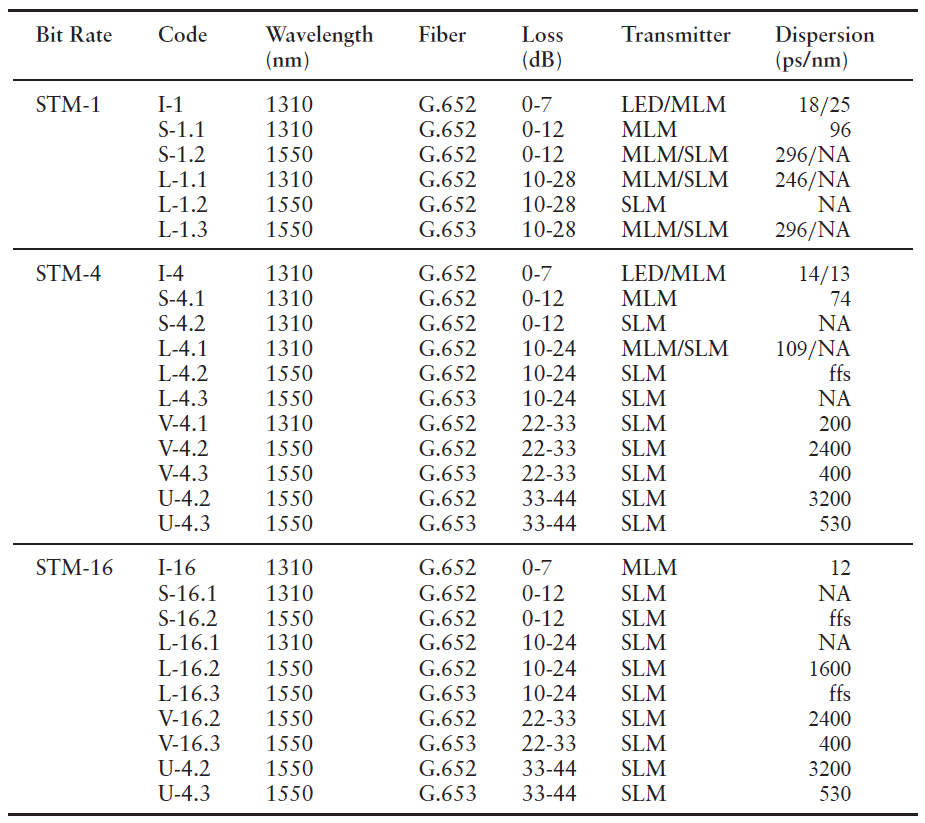
\includegraphics[scale=.5]{PhysicalSDH.png}
  \caption{Diferentes Interfaces F�sicas para SDH - ~\cite{Ramaswami2010}.}
 \label{fig:PhysicalSDH}
\end{figure}

Na Figura~\ref{fig:PhysicalSDH}, a primeira coluna referencia a taxa de transmiss�o de acordo com a hierarquia \ac{SDH}. A segunda coluna introduz uma nomenclatura que depende do comprimento do enlace, de acordo com as defini��es a seguir: \textit{Intraoffice Connections} � representado pela letra "I" e indica dist�ncias de aproximadamente 2 km; \textit{Short-haul Interoffice Connections}, que indica enlaces de dist�ncia de aproximadamente 15 km para o comprimento de onda de 1310 nm e 40 km para comprimento de onda de 1550 nm, � representada pela letra "S"; \textit{Long-haul Interoffice Connections}, representada pela letra "L" e corresponde a dist�ncia de aproximadamente 40 km para o comprimento de onda de 1310 nm e 80 km para o comprimento de onda de 1550 nm; \textit{Very-long-haul Interoffice Connections}, indicado pela letra "V" correspondendo a dist�ncia de aproximadamente 60 km para comprimento de onda de 1310 nm e 120 km para comprimento de onda de 1550 nm; \textit{Ultra-long-haul Interoffice Connections}, representado pela letra "U" e correspondendo a dist�ncias aproximadas de 160 km. O primeiro n�mero ap�s as letras indicam a qual hierarquia se est� relacionando e o segundo n�mero indica o tipo de fibra e comprimento de onda de opera��o: 1 indica opera��o em 1310 nm sobre \textit{Standard Single-Mode Fiber} (\ac{ITU-T} G.652), 2 indica opera��o em 1550 nm sobre \textit{Standard Single-Mode Fiber} (\ac{ITU-T} G.652), 3 indica opera��o em 1550 nm sobre \textit{Dispersion-shifted Fiber} (\ac{ITU-T} G.653) e 5 indica opera��o em 1550 nm e sobre \textit{Nonzero Dispersion-shifted Fiber} (\ac{ITU-T} G.655)~\cite{Ramaswami2010}. 

As outras colunas especificam o comprimento de onda de opera��o do transmissor, que pode ser em 1310 nm ou 1550 nm, o tipo de fibra �ptica a se utilizar, que pode ser \textit{Standard Single-Mode Fiber} (\ac{ITU-T} G.652), \textit{Dispersion-shifted Fiber} (\ac{ITU-T} G.653) e \textit{Nonzero Dispersion-shifted Fiber} (\ac{ITU-T} G.655), o range de perda aceit�vel, os tipos de transmissores, que podem ser \ac{LED}, \ac{MLM} ou \ac{SLM} e o range de dispers�o aceit�vel. � interessante ressaltar que ambos os ranges aceit�veis de perda e dispers�o s�o ditados pela aplica��o.
\chapter{A Rede de Transporte �tica}
\label{cap:g709}

Apesar das altas taxa de transmiss�o e escalabilidade de largura de banda proporcionada pelas redes �ticas, a tecnologia de comunica��es �tica atual possui limita��es de supervis�o e avalia��o de desempenho. Com o objetivo de contornar essas limita��es a \ac{ITU-T} definiu a Rede de Transporte �tica, Recomenda��o ITU-T G.870 (\textit{Terms and Definitions for Optical Transport Networks})~\cite{G870}, para padronizar o m�todo de transmiss�o de sinais em redes �ticas. 

O foco deste cap�tulo � o padr�o \ac{ITU-T} G.709, que define as interfaces utilizadas na rede de transporte �tica. Assim, este cap�tulo apresenta uma breve descri��o sobre arquitetura da \ac{OTN}, o padr�o G.709 e suas camadas, os principais alarmes deste padr�o e o algoritmo de corre��o de erros (\aclu{FEC} -- \ac{FEC}).

\section{Arquitetura da OTN}
\label{sec:otn_arquitetura}

A rede de transporte �tica fornece op��es de gerenciamento e de desempenho dos caminhos �ticos atrav�s de um conjunto de cabe�alhos (\aclu{OH}s -- \ac{OH}) que s�o processados � medida que o sinal � propagado nas camadas da sua arquitetura, Recomenda��o \ac{ITU-T} G.872 (\textit{Architecture of Transport Optical Networks})~\cite{G872}, a qual � composta por camadas independentes e que refletem o escopo da transmiss�o do sinal no meio �tico. A Figura~\ref{fig:otn_architecture} ilustra a subdivis�o das camadas da \ac{OTN} e os seus dom�nios de opera��o. As fun��es de cada camada est�o relacionadas da seguinte forma: 

\begin{figure}[H]
	\begin{center}
	\subfigure{
		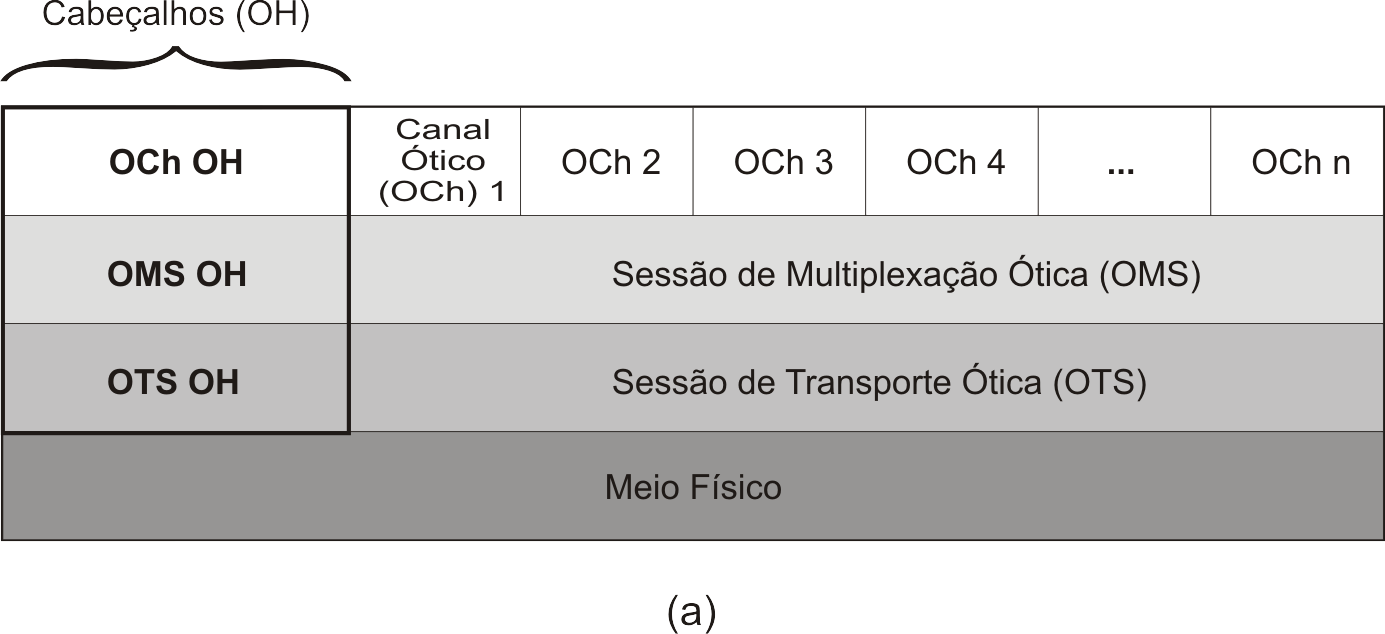
\includegraphics[scale=.9]{cap3/otn_architecture_camadas.png}
		\label{fig:otn_arq_camadas}
		}
		\subfigure{
		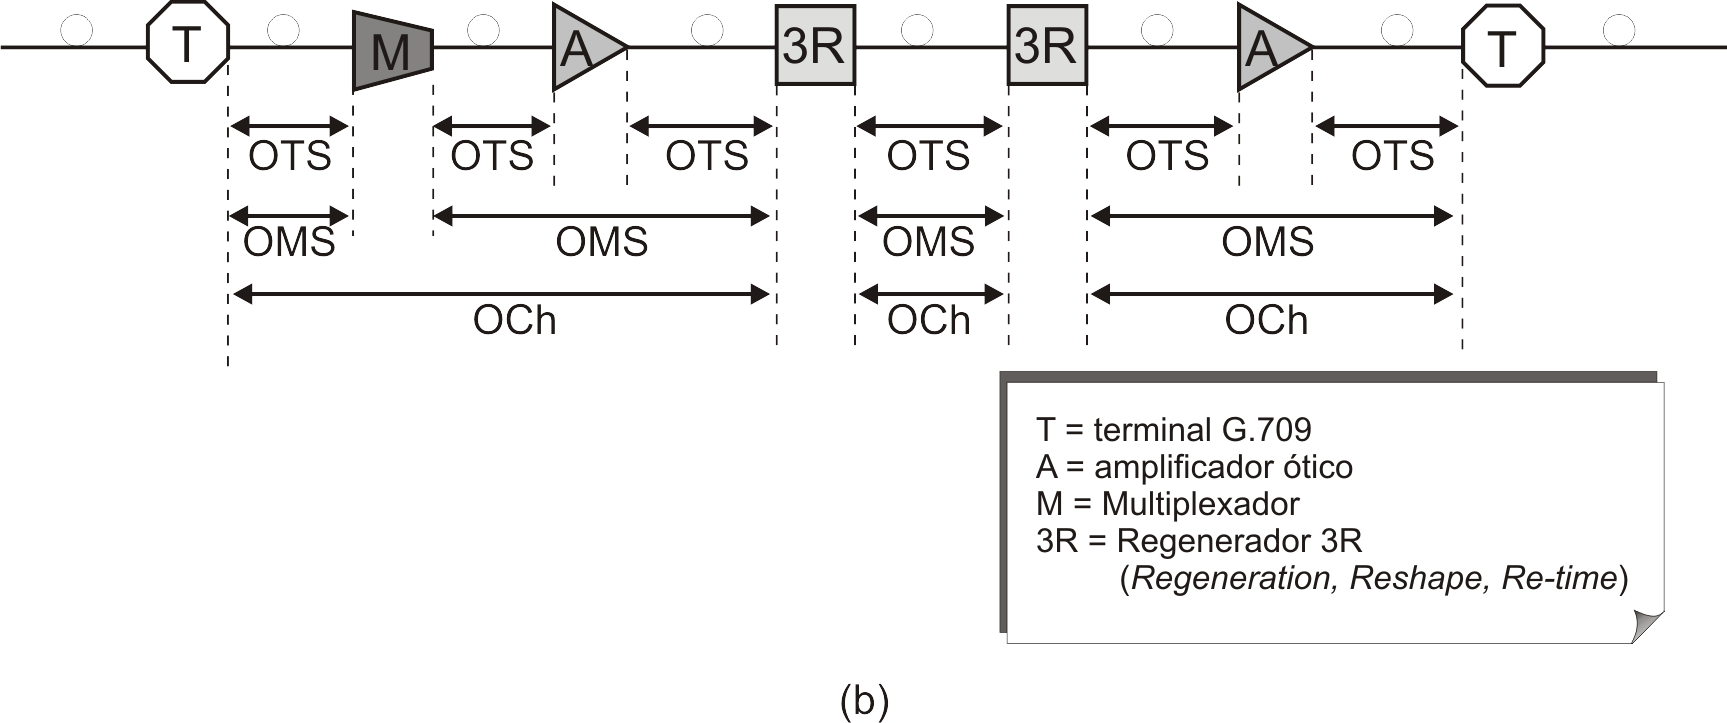
\includegraphics[scale=.9]{cap3/otn_architecture_terminations.png}
		\label{fig:otn_escopoarquitecture}
		}
		\caption{(a) Esquema da arquitetura de camadas da OTN e (b) Escopo de opera��o de cada camada em uma conex�o, que possui amplificadores e regeneradores no percurso do sinal �tico entre os terminais G.709.}
		\label{fig:otn_architecture}
	\end{center}
\end{figure}

\begin{itemize}
	\item Canal �tico (\aclu{OCh} -- \ac{OCh}): respons�vel por estabelecer a comunica��o �tica fim a fim. � nesta camada que o sinal cliente � encapsulado. Suas principais caracter�sticas s�o: (\textit{i}) o roteamento flex�vel para rearranjar conex�es; (\textit{ii}) cabe�alho que assegura a integridade do canal e (\textit{iii}) aplica��o de fun��es de opera��o, administra��o, manuten��o e provisionamento (\aclu{OAMP} -- \ac{OAMP}), como troca de par�metros de qualidade de servi�o e fun��es de sobreviv�ncia do canal �tico;
	
	\item Sess�o de multiplexa��o �tica (\aclu{OMS} -- \ac{OMS}): prov� funcionalidades para multiplexar e gerenciar um ou v�rios comprimentos de onda dentro do sinal �tico no transmissor, bem como, fun��es para separ�-los no receptor. Dentre as capacidades desta camada podemos citar: o processamento do cabe�alho que assegura a integridade da informa��o de multiplexa��o multi-comprimento de onda e a aplica��o de fun��es de opera��o e gerenciamento, como sobreviv�ncia da sess�o de multiplexa��o, por exemplo;

	\item Sess�o de transporte �tica (\aclu{OTS} -- \ac{OTS}): possui a capacidade de transmiss�o sobre v�rios tipos de m�dia �tica, como as fibras monomodo \ac{ITU-T} G.652, G.653 e G.655. Tamb�m possui um \textit{overhead} usado para fun��es de gerenciamento e sobreviv�ncia dentro desta camada;
	\item Meio f�sico: definido pelo tipo de fibra �tica usada na rede �tica, � o servidor da transmiss�o �tica.
\end{itemize}

Para permitir uma an�lise de desempenho otimizada para a transmiss�o de dados em uma rede de transporte �tica, foi desenvolvido o padr�o \textit{Digital Wrapper} ou G.709, especificado na Recomenda��o \ac{ITU-T} G.709 (\textit{Interfaces for Optical Transporte Network})~\cite{G709}, que define as interfaces, o formato do quadro e a maneira como o sinal cliente � transportado. Esse padr�o suporta diversos tipos de tecnologias clientes, tais como: \ac{SONET}/\ac{SDH}, \textit{Ethernet}, \ac{ATM}, \ac{VCAT}, \ac{GFP}. 

A recomenda��o G.709 tem recursos pr�prios de ger�ncia, monitoramento e fun��es de \ac{OAMP} baseados na experi�ncia adquirida com o uso da tecnologia \ac{SONET}/\ac{SDH}, mas foram aprimorados, o que tornou o padr�o menos complexo e mais extens�vel, pois prov� uma estrutura de cabe�alhos que permite efetuar o monitoramento e a an�lise do desempenho da rede de forma mais adequada. Al�m disso, esse padr�o emprega um robusto c�digo corretor de erros, que permite que ele seja usado em redes �ticas de longa dist�ncia. 

A arquitetura da \ac{OTN} define duas classes de interfaces de acordo com os dom�nios de aplica��o: inter-dom�nio (\aclu{IrDI} -- \ac{IrDI}) e intra-dom�nio (\aclu{IaDI} -- \ac{IaDI}), como ilustrados na Figura~\ref{fig:otn_interfaces}. Por outro lado, o \textit{digital wrapper} descreve somente as interfaces l�gicas necess�rias para transmitir a informa��o, o que n�o garante que ela seja realmente transmitida, uma vez que as especifica��es das interfaces f�sicas (�ticas e el�tricas) n�o s�o contempladas pelo padr�o~\cite{Walker2007}.

\begin{figure}[H]
 \centering
 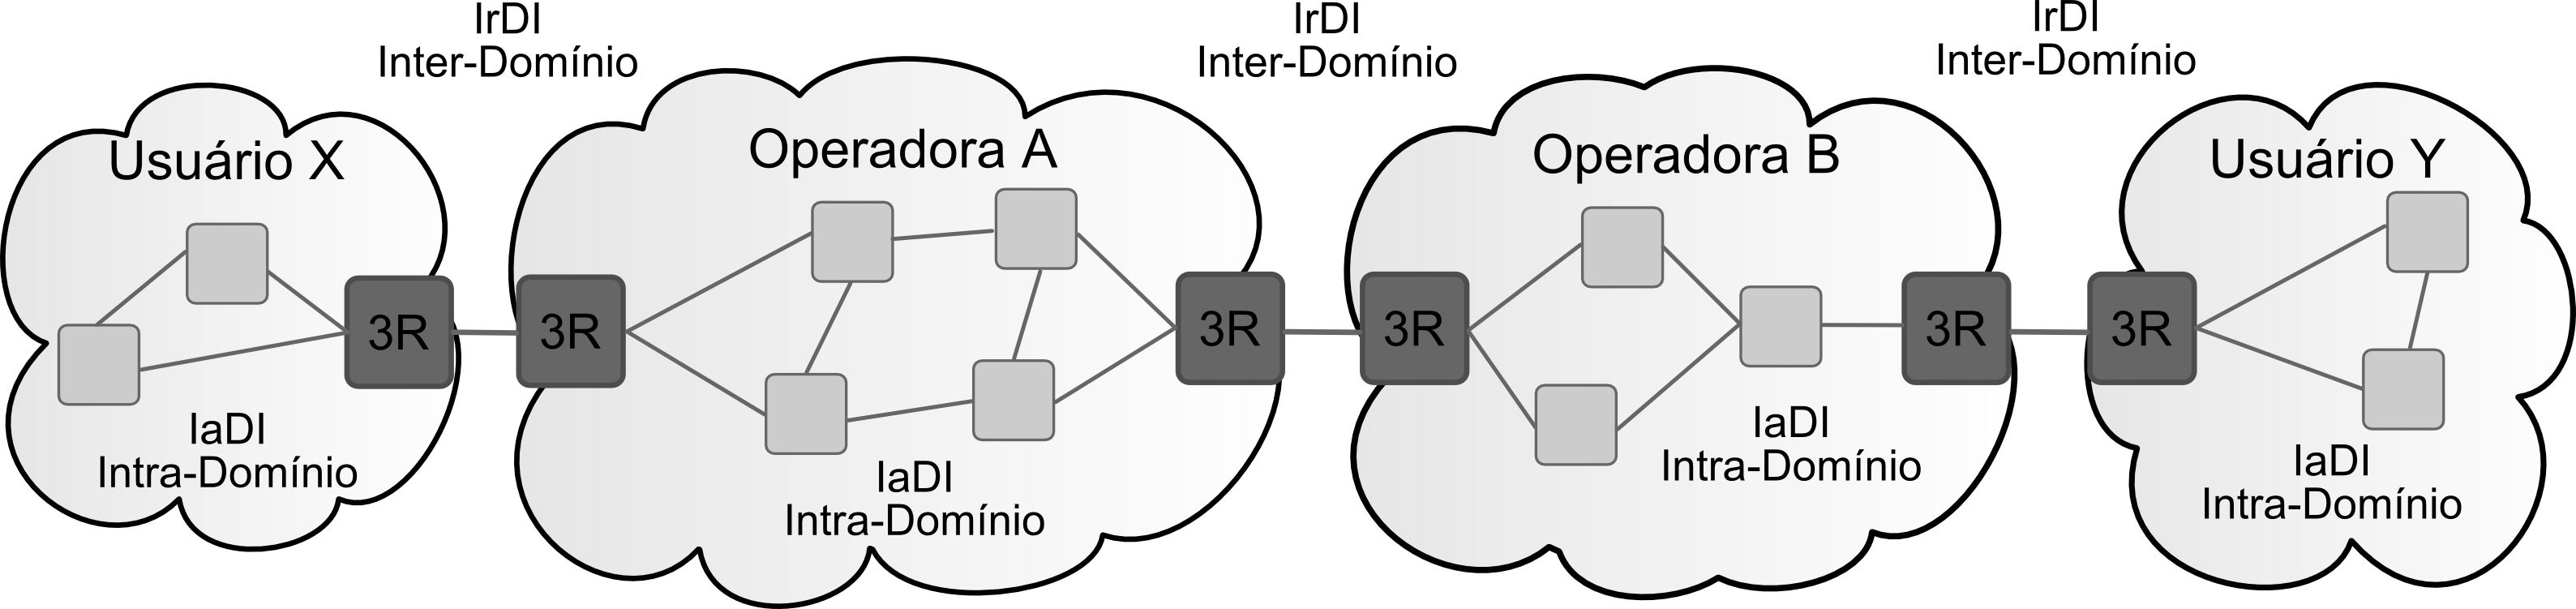
\includegraphics[scale=.6]{./cap3/interfaces.png}
 % otn_interfaces.png: 3273x873 pixel, 300dpi, 27.71x7.39 cm, bb=
 \caption{Exemplo de uma estrutura de dom�nios para interfaces da rede de transporte �tico (OTN).}
 \label{fig:otn_interfaces}
\end{figure}

Os dom�nios de aplica��o das interfaces s�o~\cite{G872}:

\begin{itemize}
      \item \ac{IrDI}: caracterizada pelo processamento 3R (regenera��o, reformata��o e retemporiza��o ou ressincroniza��o) do sinal �tico em cada uma de suas termina��es. Por exemplo, na Figura~\ref{fig:otn_interfaces}, interfaces \ac{IrDI} conectam enlaces entre as operadoras A e B ou entre a rede do usu�rio X e a operadora A.
      \item \ac{IaDI}: pertencem a um dom�nio administrativo, no qual n�o deve haver convers�o \ac{O-E-O}. Por exemplo, na Figura~\ref{fig:otn_interfaces}, s�o as interfaces internas dos dom�nios das operadoras (A e B) e dos usu�rios (X e Y).
\end{itemize}

\section{O Padr�o ITU-T G.709}
\label{sec:otn_g.709}

Al�m de tomar como exemplo a experi�ncia de monitoramento e an�lise de desempenho da tecnologia \ac{SONET}/\ac{SDH}, o G.709 tamb�m tem as taxas de transfer�ncia de suas interfaces derivadas dessa tecnologia, como � apresentado na Tabela~\ref{tab:taxas}~\cite{G709}. As interface tratam o sinal cliente como carga �til (\textit{payload}), antes de transmiti-lo pela rede �tica. Ap�s ser transmitido, o sinal �tico passa transparentemente pelos componentes do n�cleo da rede, sendo somente convertido para o dom�nio el�trico e processado digitalmente quando alcan�a o destino.

\begin{table}[H]
\begin{center}
\begin{threeparttable}
\caption{Compara��o entre as interfaces e taxas de transmiss�o das redes OTN e SONET/SDH.}
\label{tab:taxas}
\begin{tabular}{lclc} \hline
\textbf{OTN OTU$_k$} & \textbf{Taxa (Gbps)} & \textbf{SONET/SDH} & \textbf{Taxa (Gbps)}\\ \hline
OTU-1 & $2.666$ & OC-48/STM-16 & $2.488$\\ 
OTU-2 & $10.709$ & OC-192/STM-64 & $9.953$\\ 
OTU-3 & $43.018$ & OC-768/STM-256 & $39.812$\\ 
\hline
\end{tabular}
\end{threeparttable}
\end{center}
\end{table}

Antes de enviar um sinal cliente pela \ac{OTN} � feito um processamento que converte a taxa de transmiss�o do sinal cliente para a taxa da interface G.709. Por exemplo, um cliente \ac{SONET} OC-192, que possui taxa de dados de $9.953~Gbps$, ser� convertida para a interface OTU-2 (\acl{OTU} 2), que transmite dados a $10.709~Gbps$. Outras interfaces da OTN e SONET/SDH s�o comparadas na Tabela~\ref{tab:taxas}.

\begin{figure}[H]
	\centering
	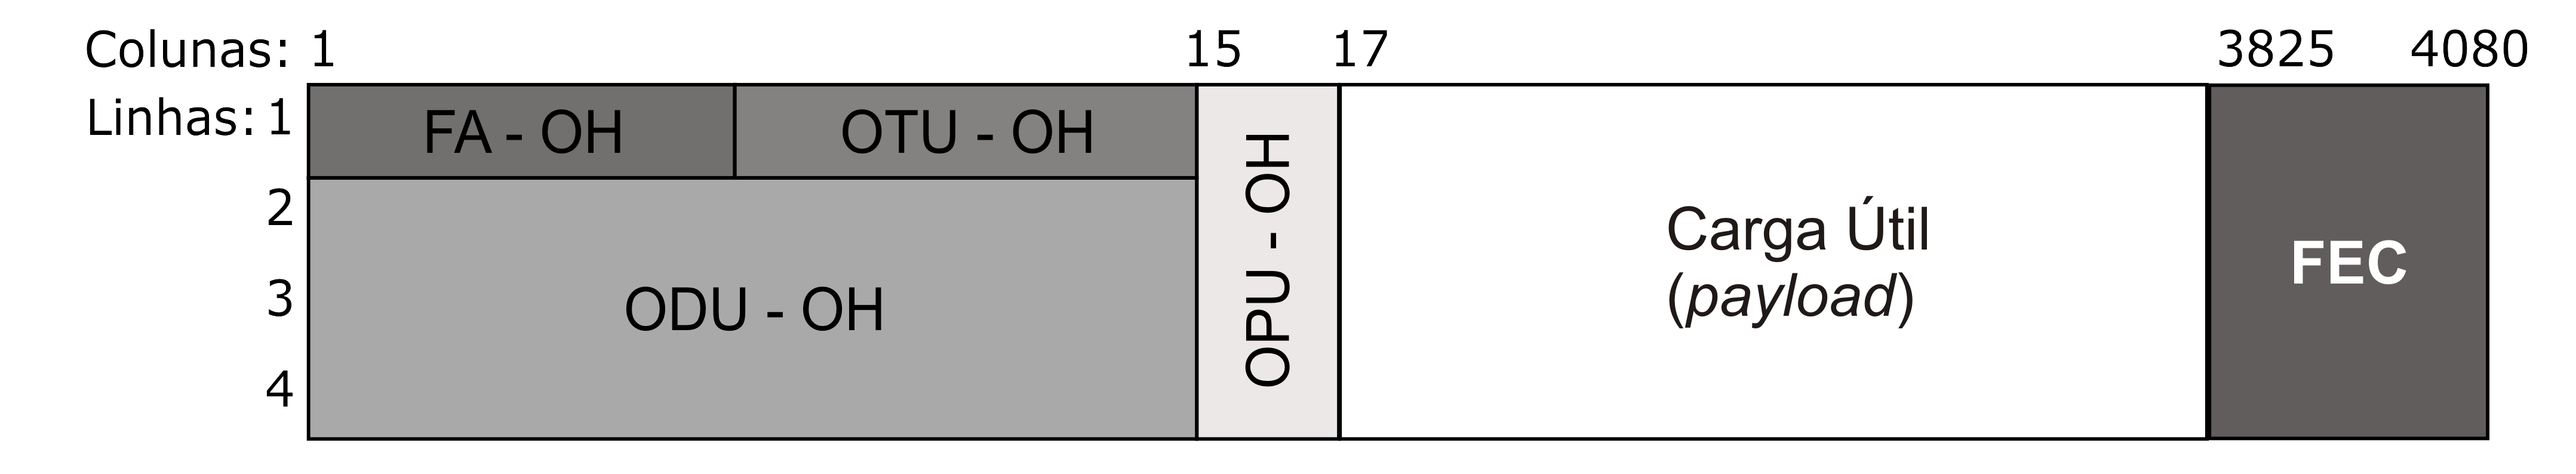
\includegraphics[scale=.9]{cap3/otn_frame2.png}
	\caption{Desenho esquem�tico do quadro da rede de transporte �tica ITU-T G.709.}
	\label{fig:otn_quadro}
\end{figure}


O G.709 armazena as informa��es sobre o sinal e seu conte�do em uma estrutura de dados chamada de quadro da \ac{OTN} (Figura~\ref{fig:otn_quadro}), que � dividido em tr�s partes principais: cabe�alho, carga �til e \ac{FEC}. O cabe�alho do quadro da \ac{OTN} possui uma �rea em que � feito o alinhamento do sinal e outros campos que correspondem a um conjunto de cabe�alhos menores, que s�o estruturados de forma hier�rquica. Esses pequenos cabe�alhos s�o definidos analisando o sinal no dom�nio el�trico ao longo do caminho e funcionam como as camadas digitais da hierarquia da \ac{OTN}. A carga �til � respons�vel por guardar as informa��es do sinal cliente e a \ac{FEC} guarda as informa��es geradas pelo c�digo corretor de erros. 

\begin{figure}[H]
	\begin{center}
		\subfigure{
			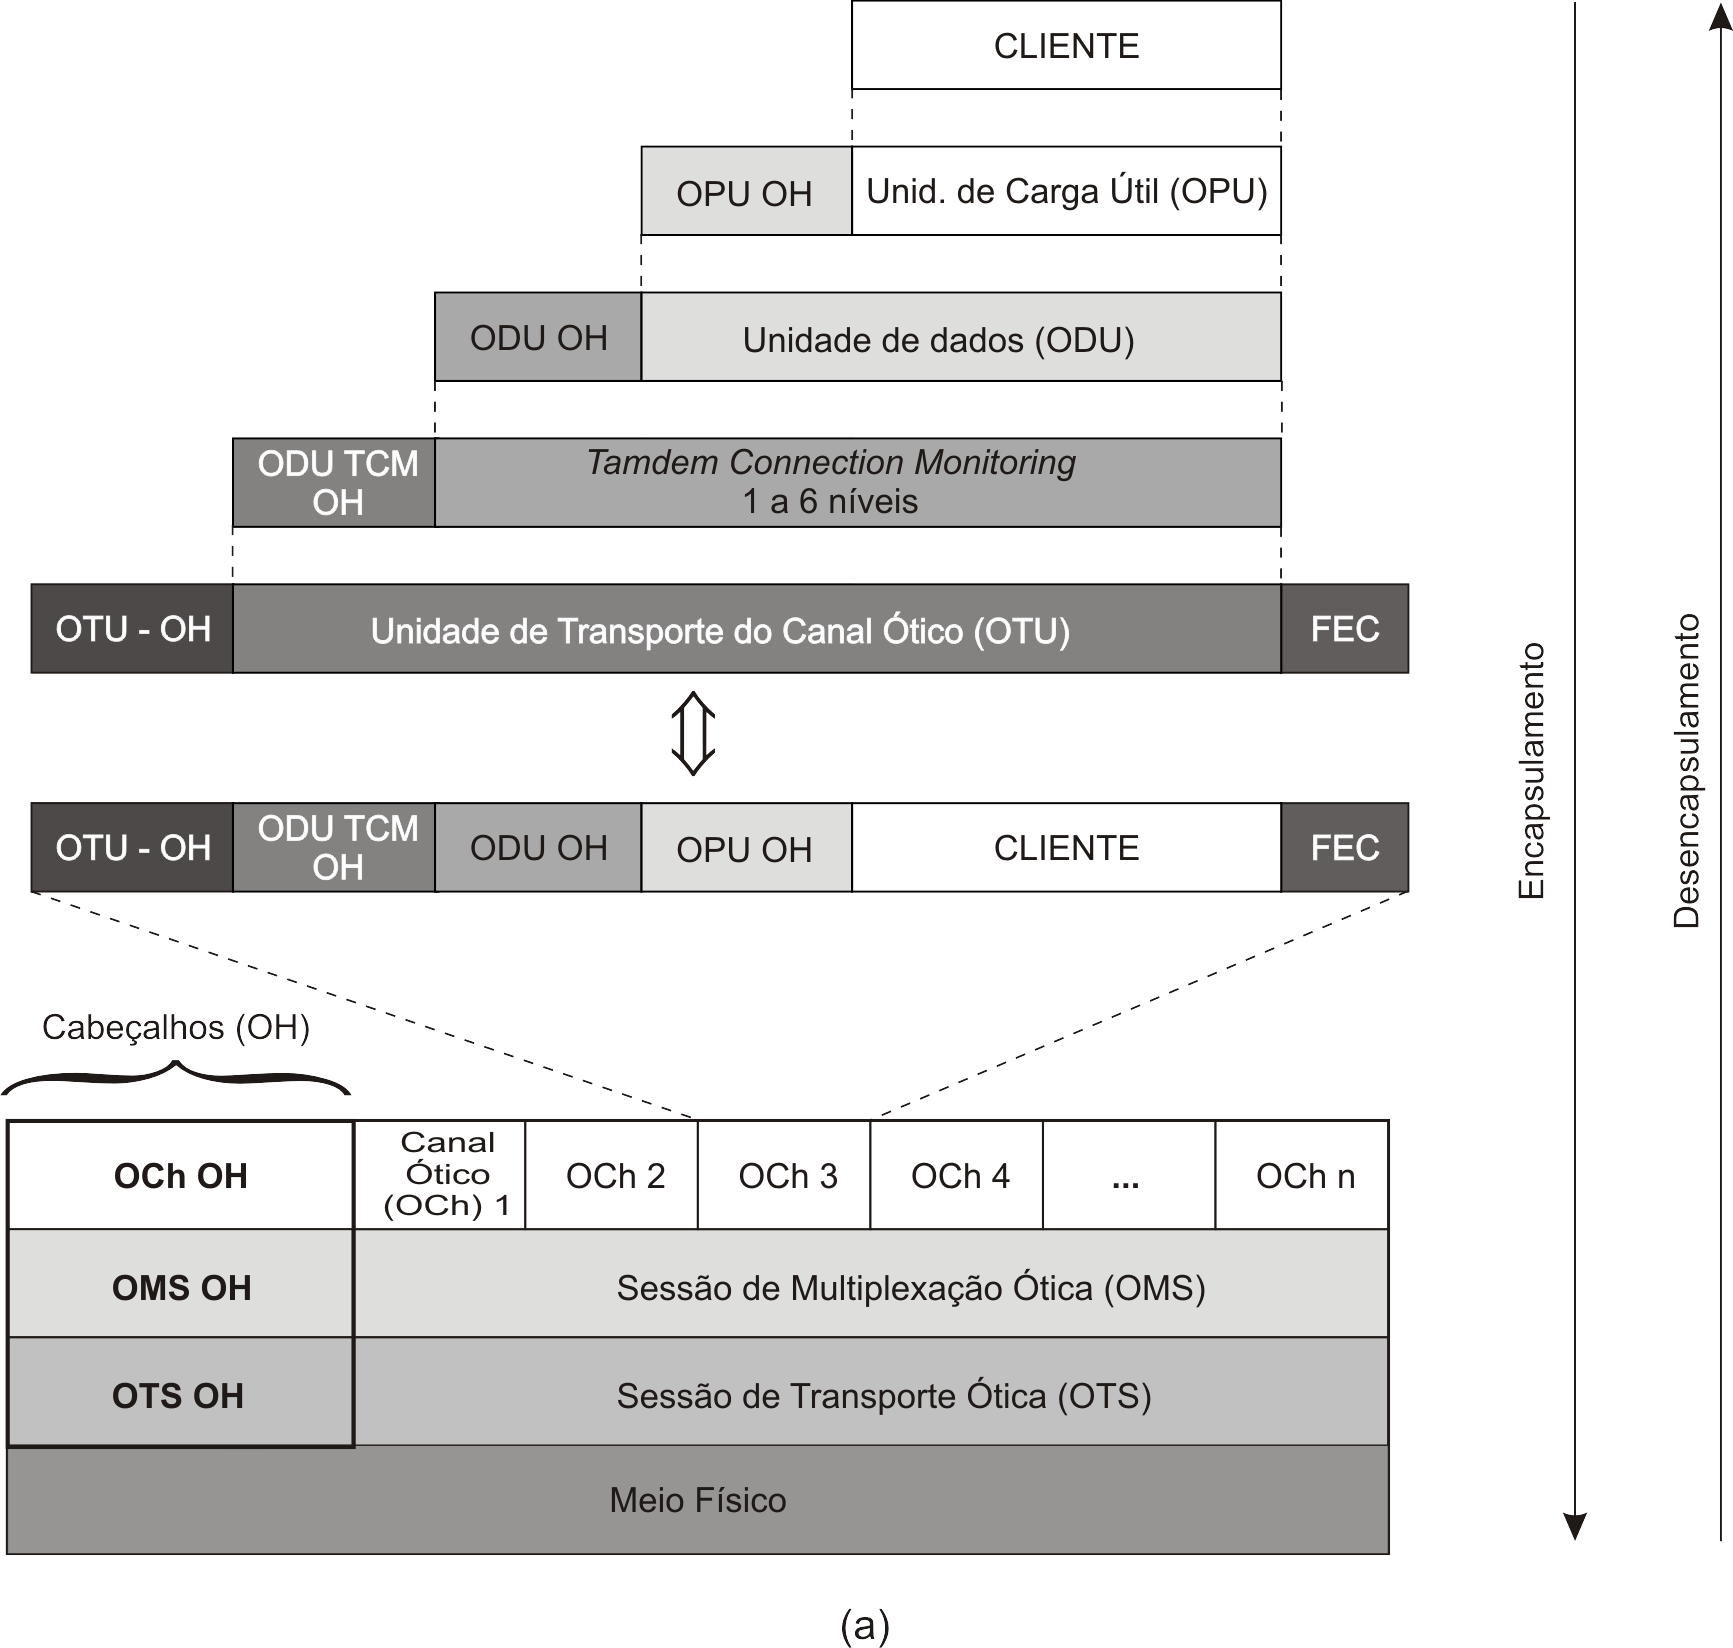
\includegraphics[scale=.8]{cap3/otn_encapsulamento.png}
			\label{fig:otn_encapsulamento}
		}
		\subfigure{
			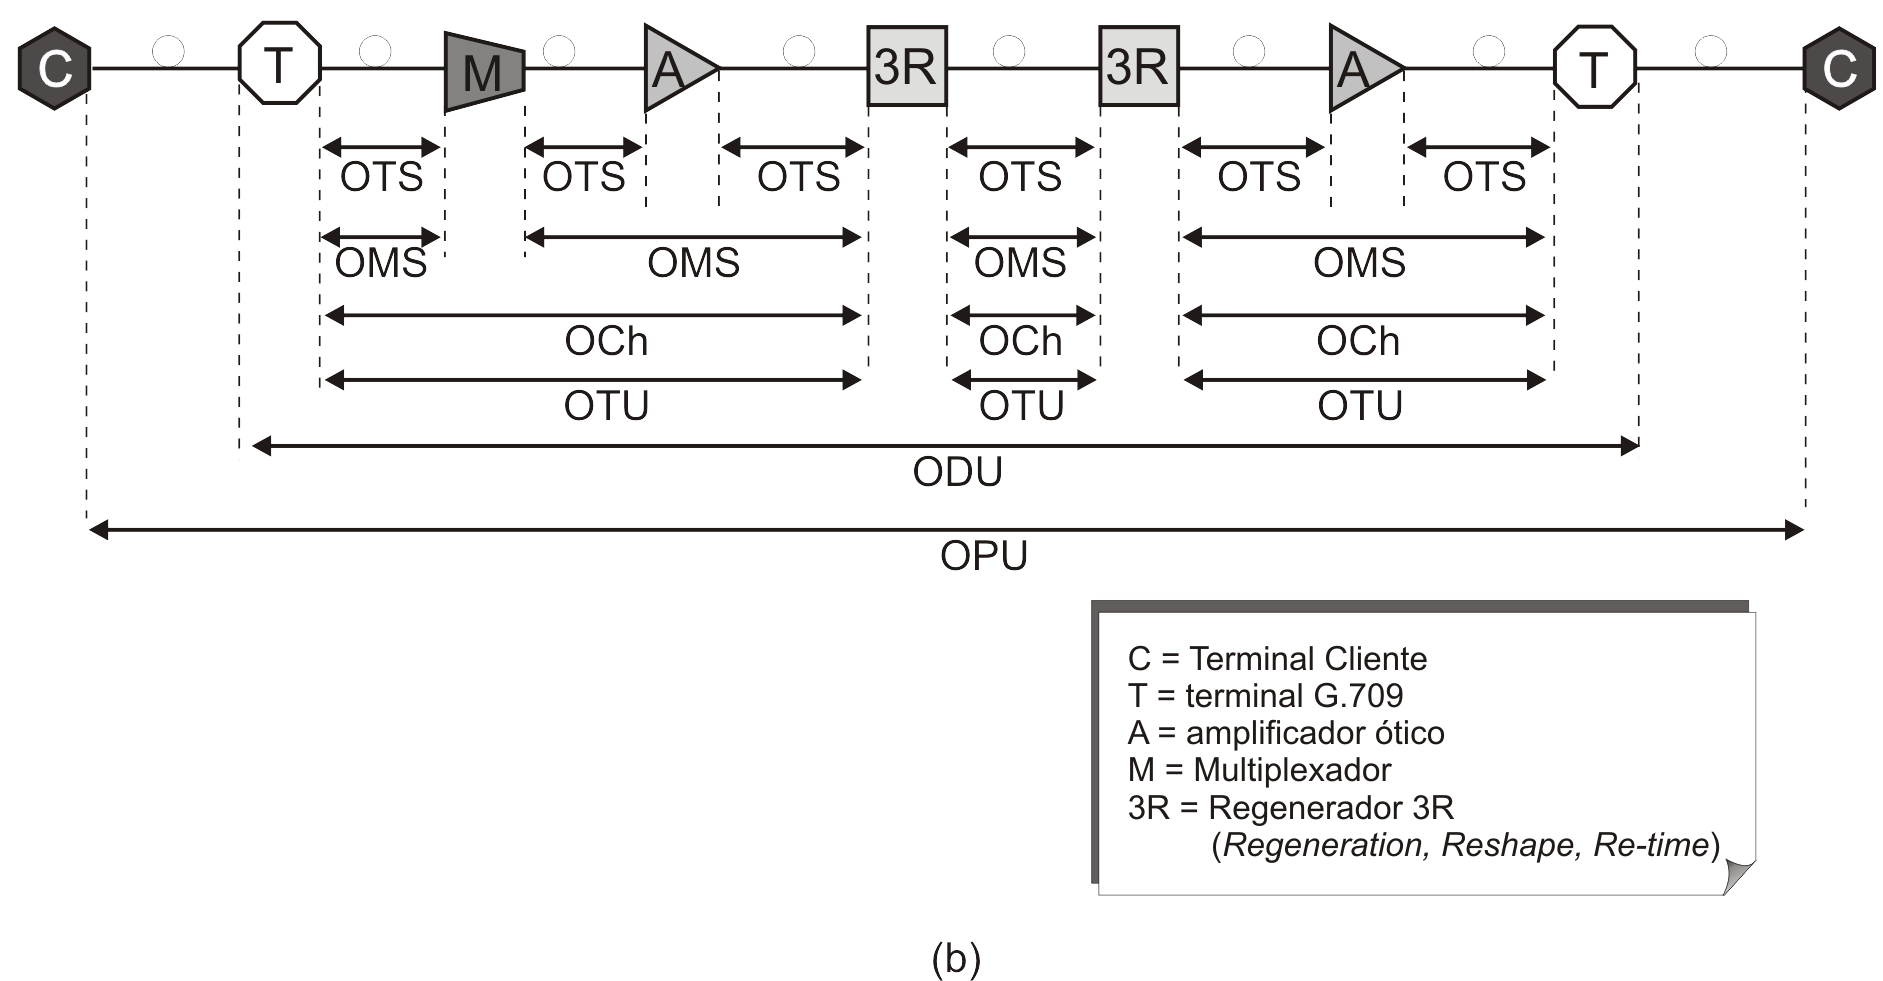
\includegraphics[scale=.8]{cap3/otn_g_709_terminations.png}
			\label{fig:otn_hierarchy_terminations}
		}
	\caption{(a) Estrutura de encapsulamento/desencapsulamento do sinal cliente na Hierarquia de Transporte �tica (OTH) da OTN e (b) Dom�nios de opera��o das camadas da OTH.}
	\end{center}
\end{figure}

De uma forma simples, o quadro da \ac{OTN} fornece op��es de monitoramento digital enquanto a arquitetura da OTN trata das op��es de monitoramento ainda no dom�nio �tico. Toda essa infraestrutura forma a Hierarquia de Transporte �tico (\aclu{OTH} -- \ac{OTH}), que � organizada em camadas como ilustrado na Figura~\ref{fig:otn_encapsulamento}, com os dom�nios de opera��o de cada camada exibidos na Figura~\ref{fig:otn_hierarchy_terminations}. As camadas da \ac{OTH} s�o divididas em:

\begin{itemize}
  \item Unidade de carga �til do canal �tico (\aclu{OPU} -- \ac{OPU});
  \item Unidade de dados do canal �tico (\aclu{ODU}-- \ac{ODU});
  \item Unidade de transporte do canal �tico (\aclu{OTU} -- \ac{OTU});
  \item Canal �tico (\acs{OCh});
  \item Sess�o de multiplexa��o �tica (\acs{OMS});
  \item Sess�o de transporte �tico (\acs{OTS}).
\end{itemize}

O protocolo G.709 encapsula o sinal do cliente no quadro na OTN. Para isto, o sinal � adicionado na �rea de carga �til \ac{OPU} e tem suas informa��es inseridas no cabe�alho da unidade de carga �til (OPU-OH). Logo, o OPU e seu cabe�alho s�o mapeados no cabe�alho do \ac{ODU} (ODU-OH), que por sua vez, tem suas informa��es mapeadas no cabe�alho do \ac{OTU} (OTU-OH). O encapsulamento � ilustrado na Figura~\ref{fig:otn_encapsulamento}. Ap�s essa etapa, o sinal � transmitido utilizando-se um dado comprimento de onda. � medida que o dom�nio de opera��o de camada da OTH � atingido, os cabe�alhos s�o desencapsulados e suas fun��es s�o ativadas. 

A Figura~\ref{fig:otn_hierarchy_terminations} apresenta os dom�nios de opera��o das camadas da OTH. O dom�nio de opera��o do \ac{OPU} limita-se aos terminais cliente da OTN. A unidade de dados (\ac{ODU}) � utilizada somente por terminais que suportam o G.709 e tem a fun��o de monitorar caminho �tico fim a fim. Por outro lado, a unidade de transporte (\ac{OTU}) tem a habilidade de converter o sinal cliente para o dom�nio �tico e fazer o monitoramento entre os terminais G.709 e regeneradores. Al�m disso, o OTU permite que o sinal �tico seja regenerado eletronicamente sem que seja necess�rio ler o sinal cliente. Desta forma, o OTU preocupa-se somente com o monitoramento da sess�o entre terminais G.709 e regeneradores, bem como entre regeneradores. Ao visualizar a Figura~\ref{fig:otn_hierarchy_terminations} ainda pode-se observar os escopos de transmiss�o das camadas que est�o no dom�nio �tico (\ac{OCh}, \ac{OMS} e \ac{OTS}). Assim, ao alcan�ar o terminal de destino G.709 o sinal cliente � desencapsulado encaminhado para o terminal de destino da tecnologia cliente da \ac{OTN}. 

\begin{figure}[H]
	\centering
	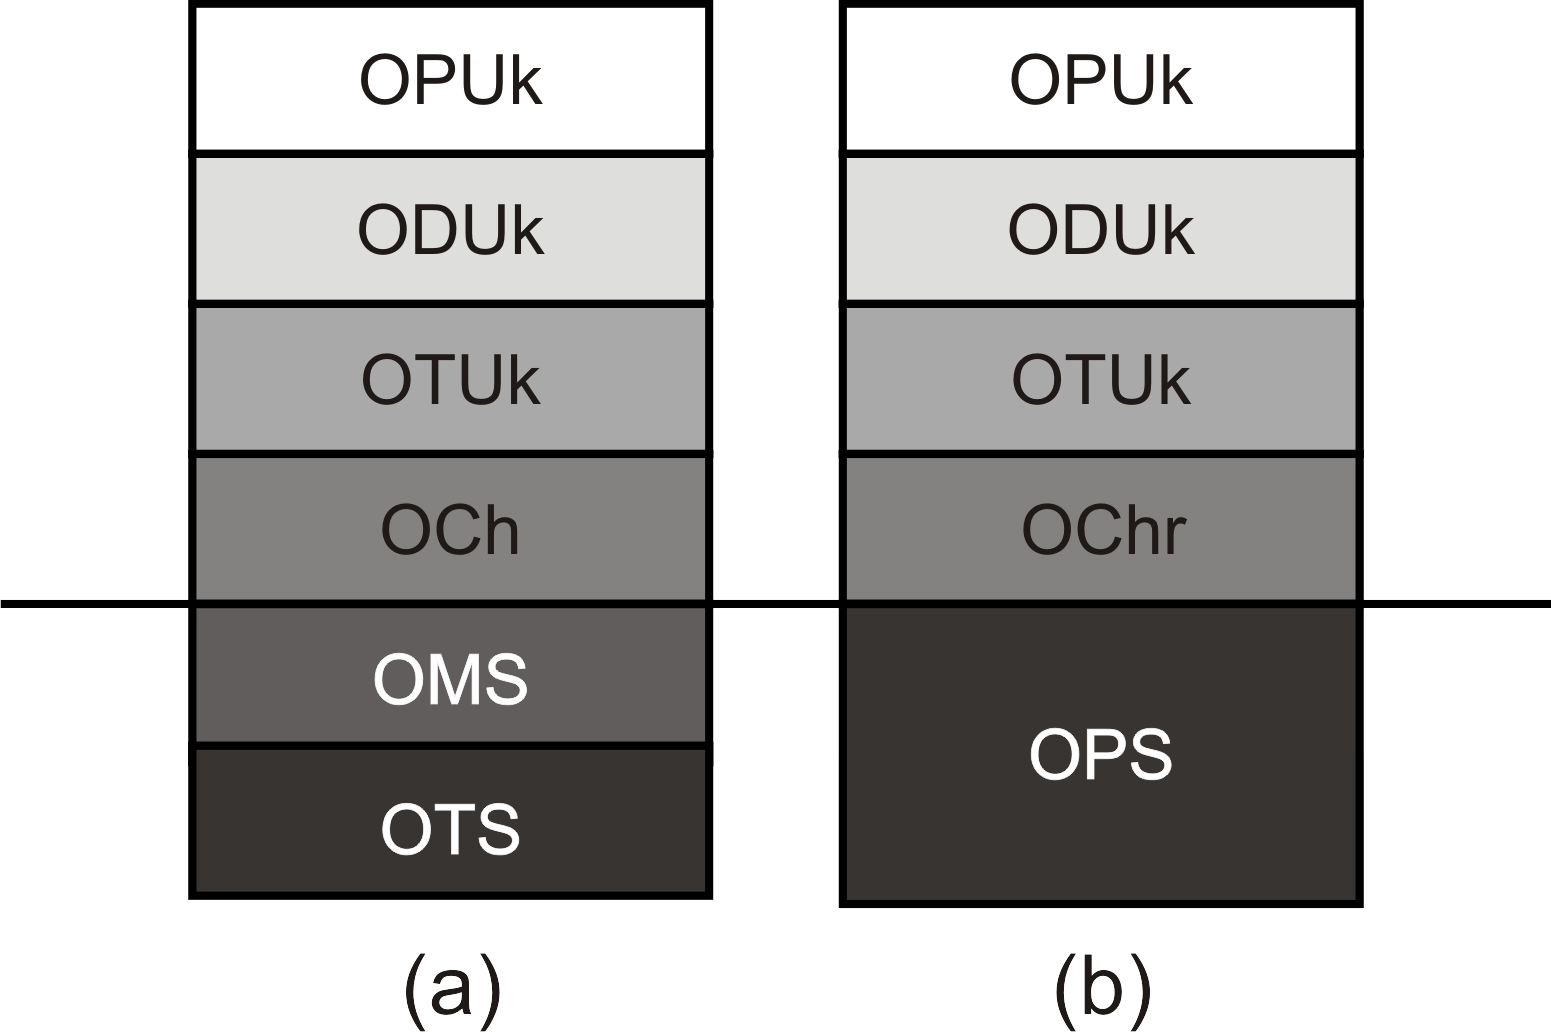
\includegraphics[scale=1]{./cap3/otn_hierarchy_reduction}
	\caption{Comparativo entre as Hierarquias da OTN: (a) Estrutura camadas da OTH com funcionalidades reduzidas do padr�o ITU-T G.709 e (b) camadas da OTH baseadas na arquitetura da OTN definida na recomenda��o ITU-T G.872.}
	\label{fig:otn_hierarchy_reduction}
\end{figure}

O G.709 tamb�m especifica uma hierarquia de transporte com capacidade e fun��es de gerenciamento reduzida na camada �tica. Para isto, uma nova camada Sess�o F�sica �tica (\aclu{OPS} -- \ac{OPS}), que substitui as camadas \ac{OMS} e \ac{OTS} da \ac{OTH}. A \ac{OPS} tamb�m utiliza um canal �tico com capacidade reduzida (\aclu{OChr} -- \ac{OChr}). A Figura~\ref{fig:otn_hierarchy_reduction} exibe as estruturas das hierarquias suportadas. Consequentemente, a infraestrutura do G.709 traz as seguintes vantagens para as redes �ticas~\cite{Walker2007}: (\textit{i}) menor complexidade no transporte de aplica��es em rela��o a tecnologia SONET\slash SDH; (\textit{ii}) cabe�alho otimizado para transportar o sinal cliente sobre um canal \ac{WDM}; (\textit{iii}) redu��o dos custos operacionais; (\textit{iv}) capacidade de multiplexar duas vezes mais largura de banda que a tecnologia SONET\slash SDH, tornando-se mais escal�vel para taxas maiores e (\textit{v}) maior custo-benef�cio por suportar diferentes tipos de tecnologias de transporte como \textit{Ethernet} e \ac{SAN}; (\textit{vi}) utiliza��o de c�digo corretor de erros; (\textit{vii}) maior quantidade de n�veis de monitoramento por meio do \ac{TCM} e (\textit{viii}) preserva��o do cabe�alho e transmiss�o transparente do sinal cliente.

\subsection{�rea de Alinhamento do Quadro da OTN}

A �rea de alinhamento do quadro (\aclu{FA} -- \ac{FA}) � o campo de cabe�alho (FA-OH) utilizado para identificar o in�cio e o fim dos quadros da \ac{OTN} recebidos. A figura Figura~\ref{fig:otn_fa_oh} ilustra a estrutura de cabe�alhos do quadro da OTN e apresenta em detalhes os subcampos do FA-OH. Tais subcampos s�o:

\begin{figure}[H]
 \centering
 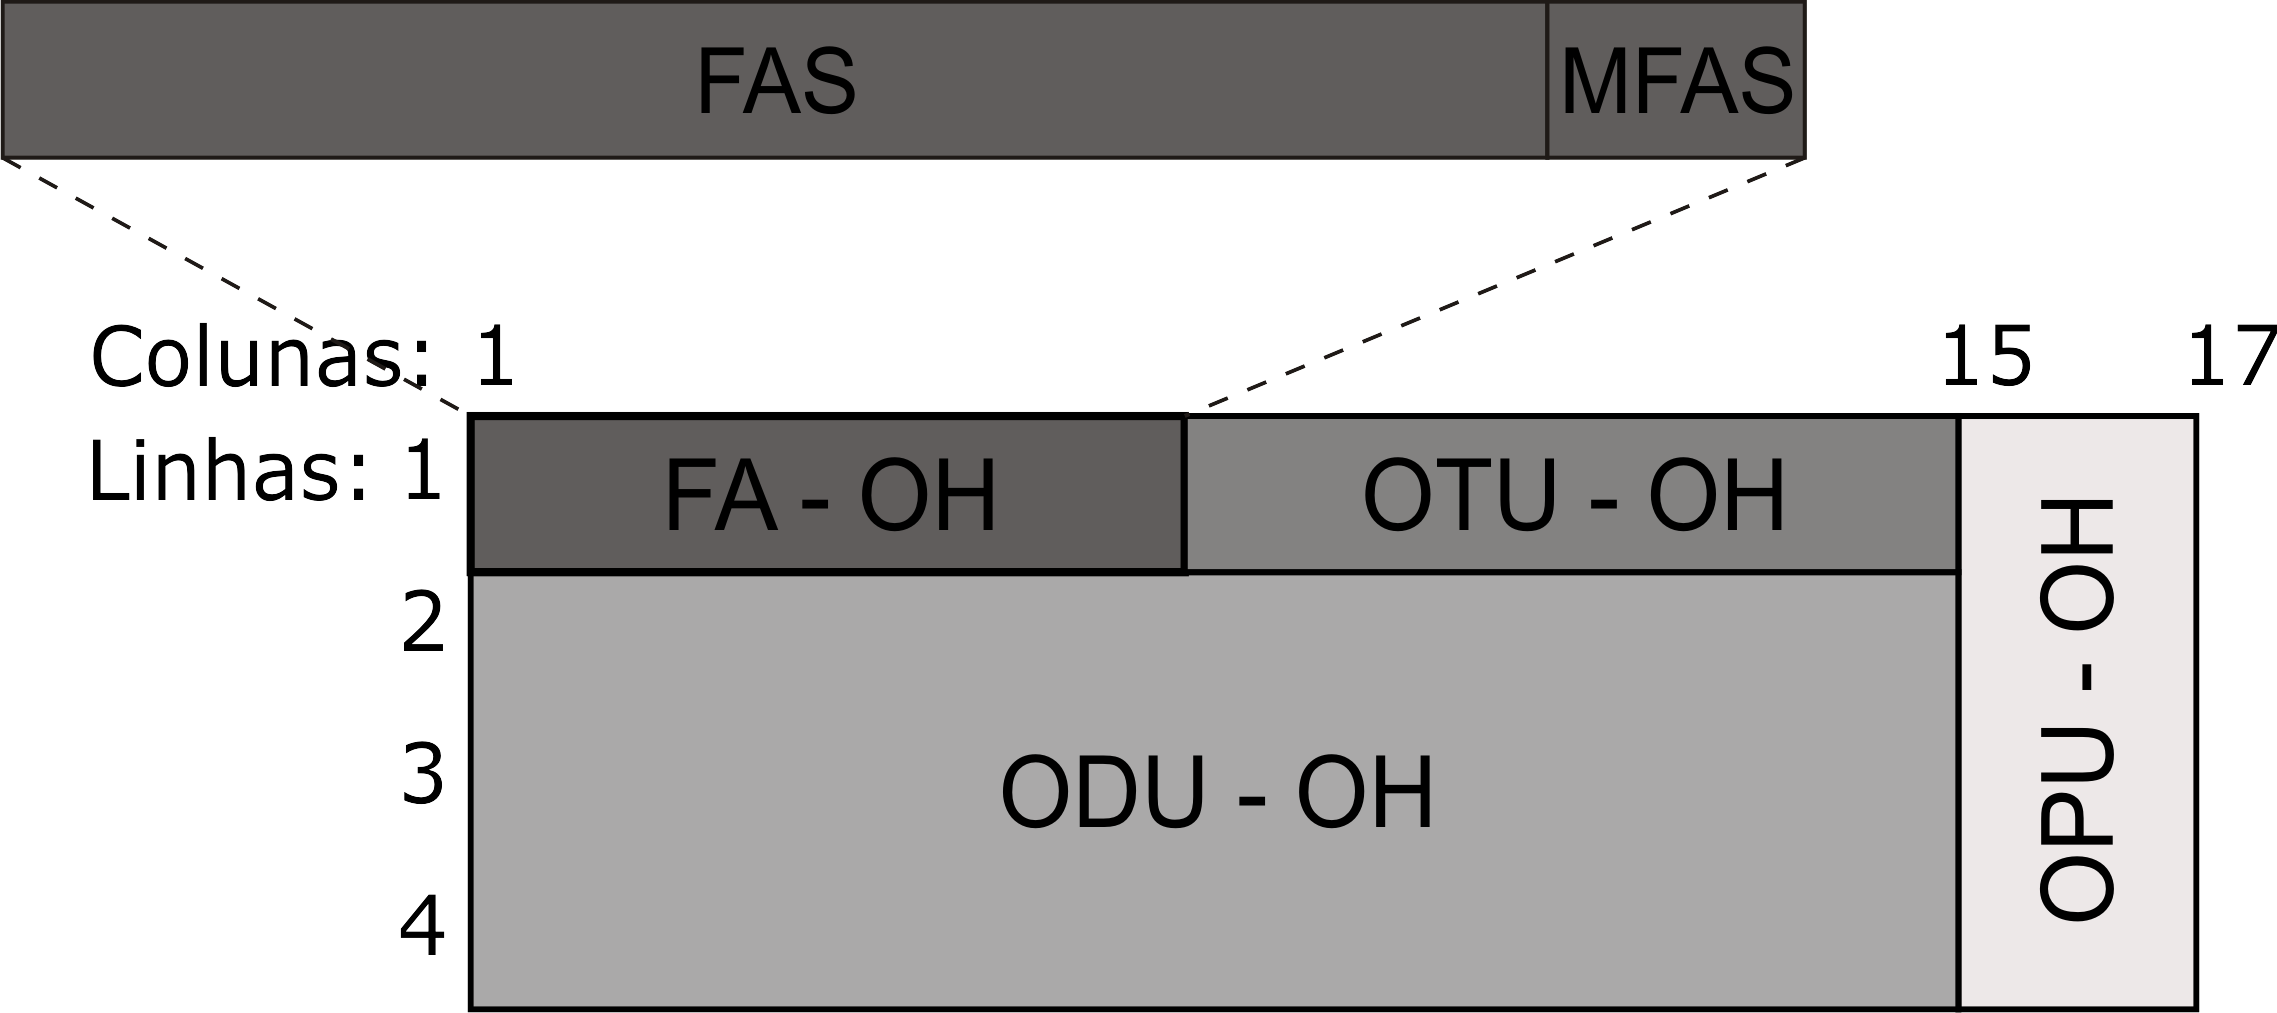
\includegraphics[scale=.9]{./cap3/otn_fa_oh.png}
 \caption{Estrutura dos subcampos (FAS e MFAS) da �rea de alinhamento (FA-OH) em evid�ncia no quadro da OTN.}
 \label{fig:otn_fa_oh}
\end{figure}

\begin{itemize}
	\item \ac{FAS}: campo de seis \textit{bytes} que permite identificar o tamanho do quadro, bem como tem a habilidade de detectar condi��es como \ac{OOF} e \ac{LOS}, caso os dados recebidos n�o cumpram os requisitos do equipamento. Este \textit{bytes} n�o s�o embaralhados na transmiss�o;
	\item \ac{MFAS}: campo de um \textit{byte} que � usado para contar a quantidade de quadros da \ac{OTN} que s�o gerados a partir do sinal cliente. Com esse recurso � poss�vel a cria��o de um ``grande quadro'' formado por 256 quadros.
\end{itemize}

Durante o processamento do sinal para o seu envio, todos dados nos campos do quadro da \ac{OTN} s�o serializados por um m�todo de embaralhamento (\textit{scrambling}), exceto os \textit{bytes} contidos no campo \ac{FAS}.


\subsection{A unidade de transporte do canal �tico (OTU)}
\label{sub:otu}

O cabe�alho da unidade de transporte do canal �tico (OTU-OH) � capaz de fazer o monitoramento de uma sess�o da conex�o, que � definida como o segmento da conex�o compreendido entre pontos de convers�o \ac{O-E-O}. O OTU-OH est� organizado da seguinte forma (Figura~\ref{fig:otn_otu_oh}):

\begin{figure}[H]
 \centering
 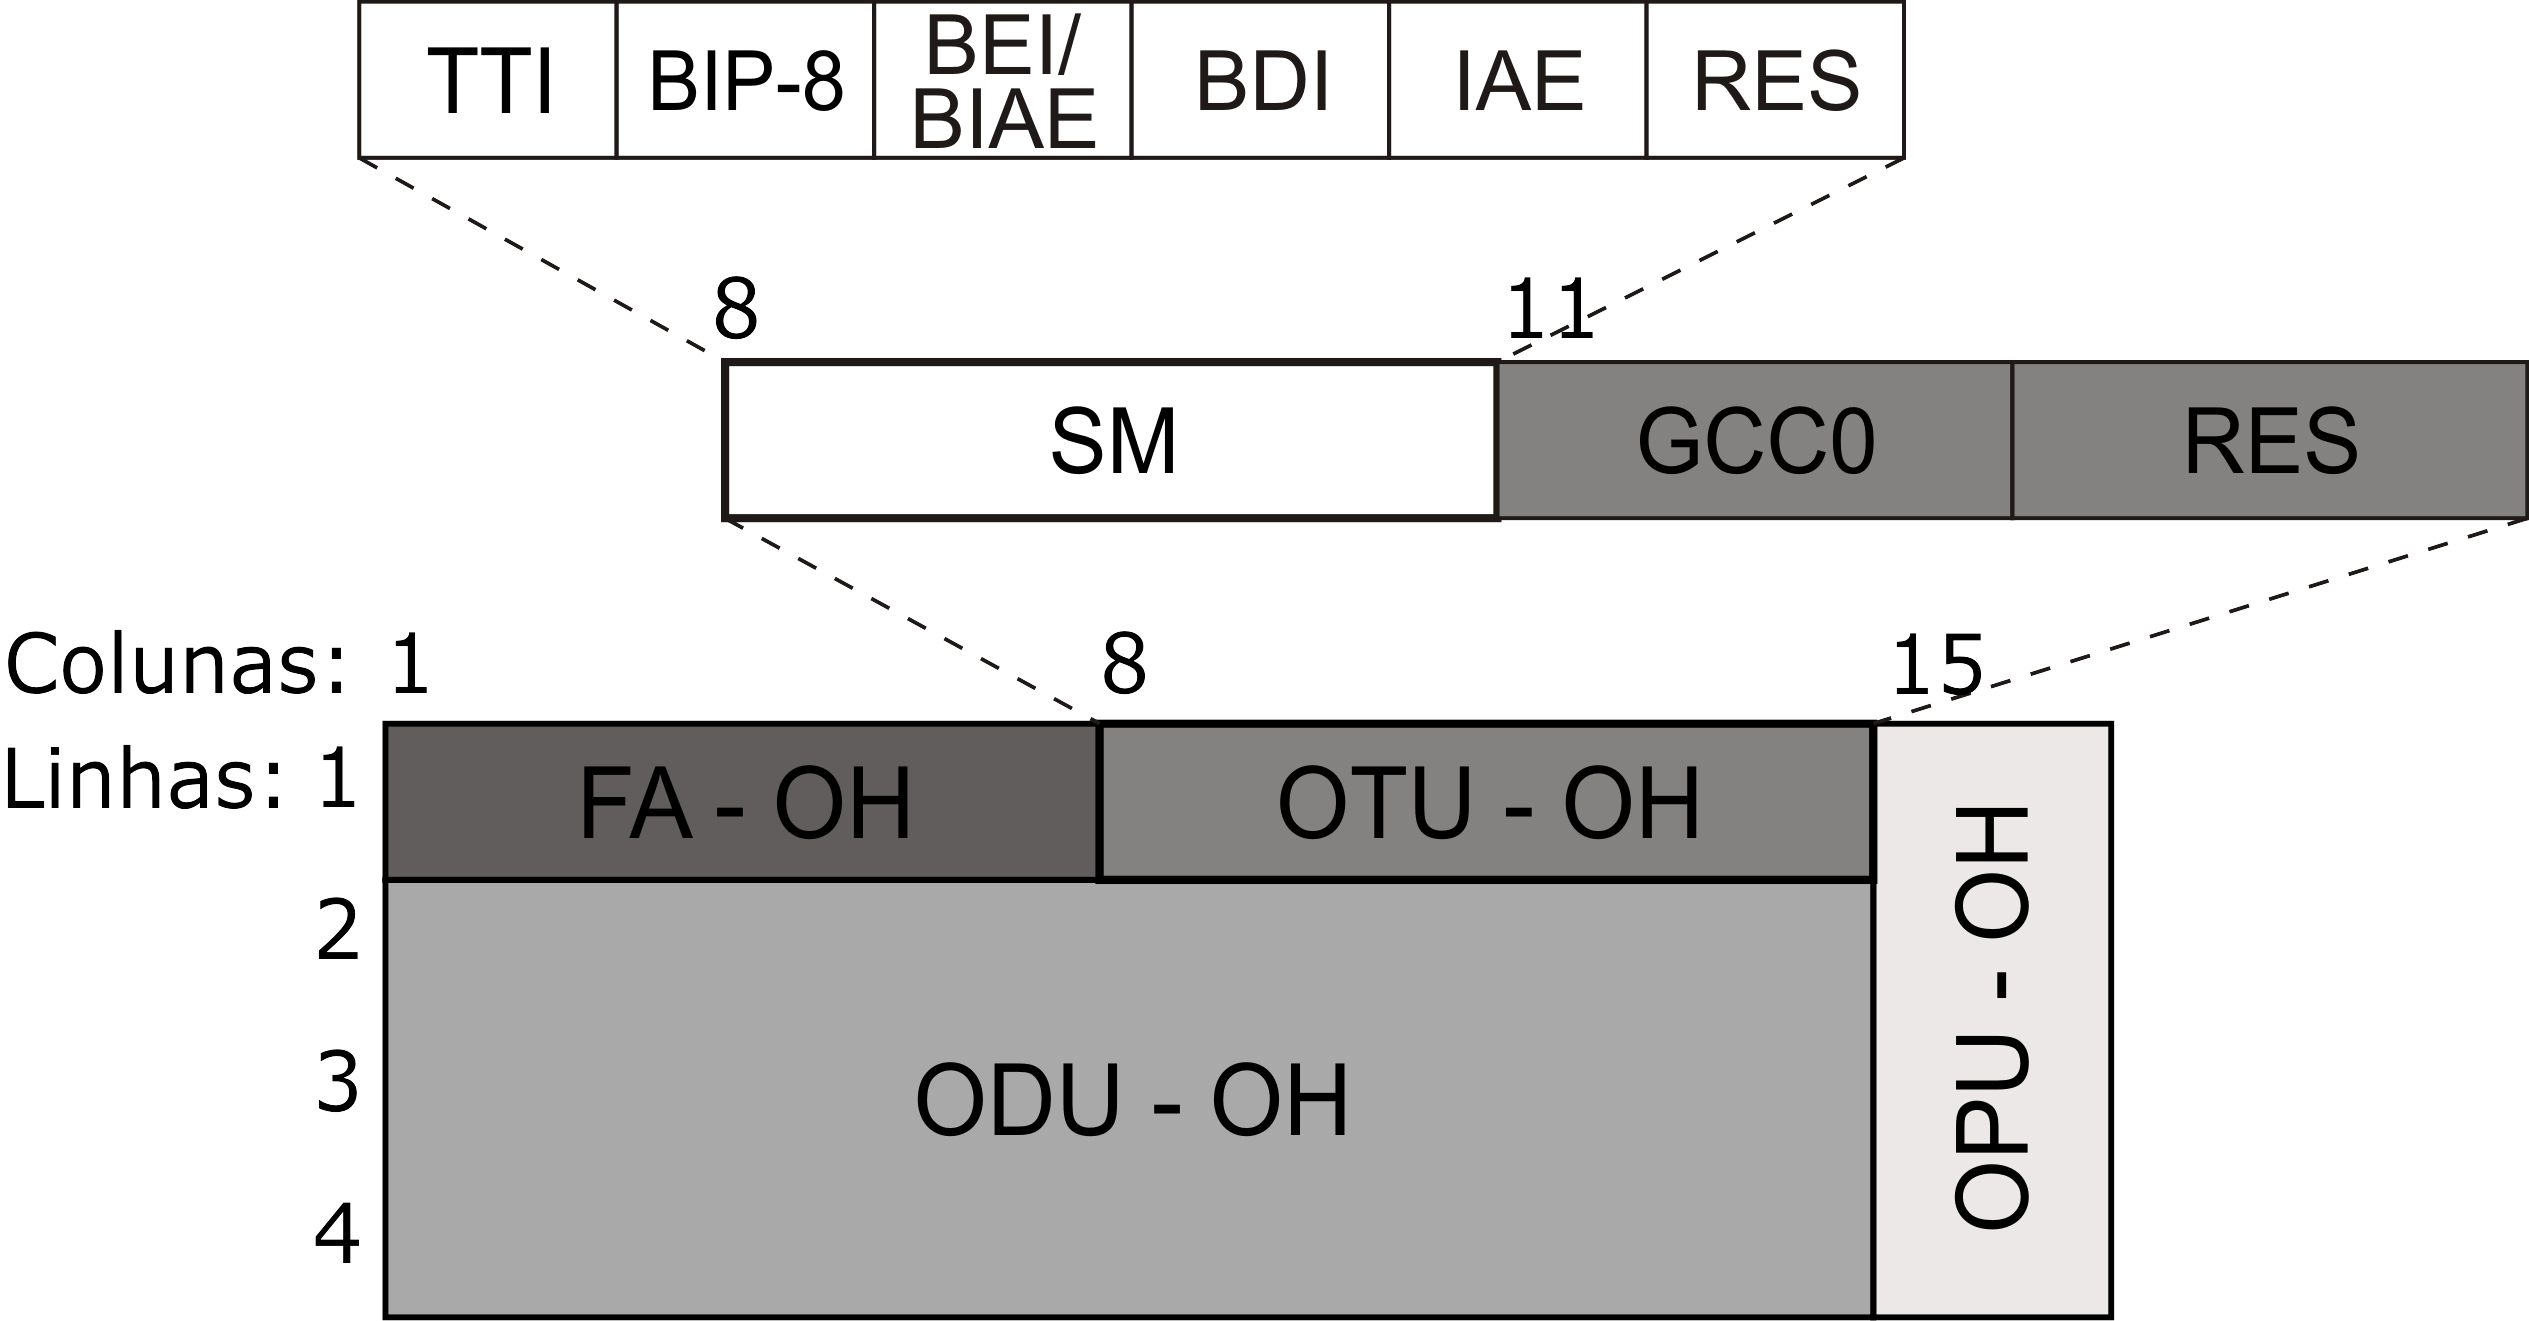
\includegraphics[scale=.7]{./cap3/otn_otu_oh.png}
 \caption{Estrutura de campos do cabe�alho do OTU com o subcampo SM em evid�ncia.}
 \label{fig:otn_otu_oh}
\end{figure}

\begin{itemize}
 \item \ac{SM}: faz o monitoramento entre conex�es totalmente �ticas. Possui os seguintes subcampos: (\textit{i}) o \ac{TTI} cont�m os identificadores para terminais de acesso de origem e destino da conex�o;
(\textit{ii}) o \ac{BIP-8} transporta um c�digo de paridade contendo 8 \textit{bits}. Este c�digo � calculado sobre os \textit{bytes} que comp�em o \ac{OPU}. Se erros forem encontrados ao recuperar a informa��o do \ac{BIP-8}, o n�mero de \textit{bits} errados s�o transmitidos para o transmissor dentro segundo quadro subsequente ($frame~i+2$) atrav�s do campo \acs{BEI}; (\textit{iii}) o \ac{BEI} / \ac{BIAE} informa ao transmissor a quantidade de blocos do \ac{BIP-8} que est�o com erros ou sobre o status do campo \acs{IAE}; (\textit{iv}) o \ac{BDI} � usado pelo destinat�rio para informar ao transmissor sobre o status do sinal recebido e (\textit{v}) o \ac{IAE} permite que o terminal transmissor informe ao receptor sobre o alinhamento do sinal. Este campo cont�m somente um \textit{bit}, o valor 1 � utilizado em caso de erro;
  \item \aclu{GCC} 0 (\ac{GCC}0): este campo serve como um canal de comunica��o que pode ser usado para transmitir informa��es entre termina��es \ac{OTU};
  \item RES: campo reservado para futura padroniza��o.
 \end{itemize}

\subsection{A unidade de dados do canal �tico (ODU)}
\label{sub:odu}

Diferentemente do OTU-OH, o cabe�alho da unidade de dados do canal �tico (ODU-OH) tem como fun��o analisar o caminho fim a fim entre uma fonte e um destino, sem se preocupar em monitorar regenera��es \ac{O-E-O} do sinal. Assim, o m�todo de monitoramento executado pelo \ac{ODU} � bem semelhante ao \ac{OTU}, possuindo inclusive, os mesmos campos utilizados para alarmes. A organiza��o do ODU-OH � ilustrado na Figura~\ref{fig:otn_odu_oh} e seus campos s�o:

\begin{figure}[H]
 \centering
 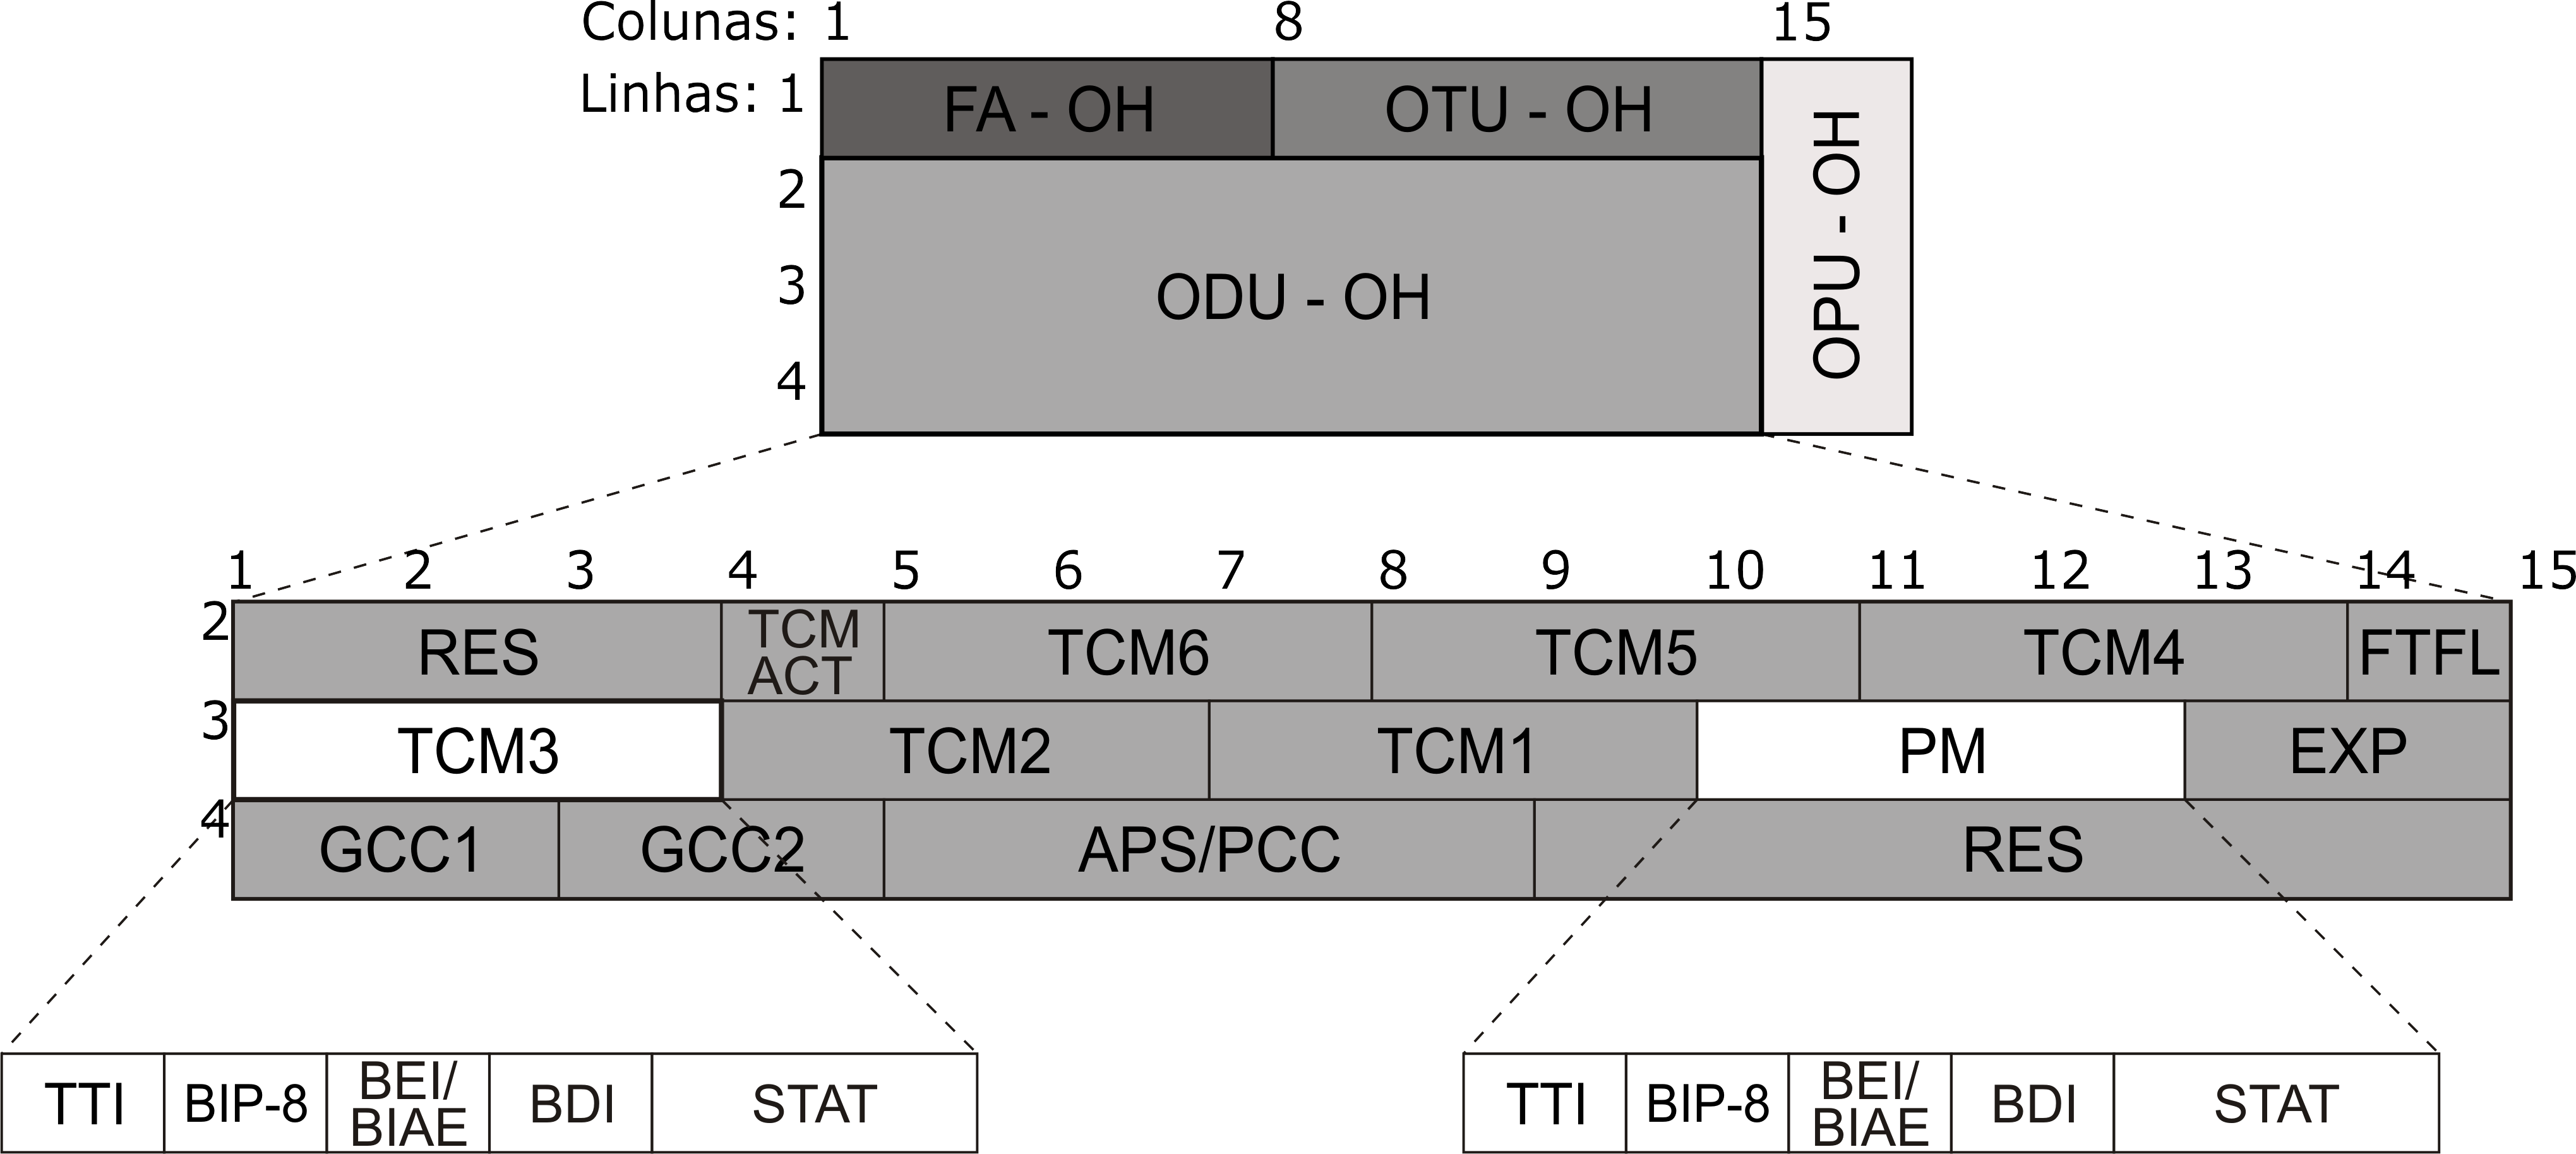
\includegraphics[scale=.7]{./cap3/otn_odu_oh.png}
 \caption{Estrutura de subcampos do cabe�alho do ODU com os subcampos do PM e TCM3 em evid�ncia.}
 \label{fig:otn_odu_oh}
\end{figure}

\begin{itemize}
	\item \ac{PM}: possui uma estrutura similar ao campo \acf{SM} do \ac{OTU}, exceto pelo subcampo STATS, que indica o status do caminho e consiste em informar se h� presen�a ou aus�ncia de sinal;
	\item \ac{TCM}$i$: Consiste em seis diferentes n�veis de monitoramento que podem ser utilizados de acordo com os dom�nios administrativos utilizados pelo que sinal �tico. Esses campos possuem a mesma estrutura do \acf{PM}. Assim, cada \ac{TCM} pode ser usado para monitorar um subcaminho que pertence a um ou mais dom�nios administrativos dentro do caminho fim a fim.
	\item \ac{TCM} ACT (\ac{TCM} \textit{activation/deactivation}): foi proposto de ser usado para ativa��o ou desativa��o dos campos \ac{TCM}, sendo que esta funcionalidade ainda n�o est� definida no padr�o G.709;
	\item \ac{FTFL}: � usado para informar sobre o tipo e o local da falha. Este campo cont�m 256 \textit{bytes} e informa se a falha ocorreu durante o encaminhamento (\textit{forward}) ou durante o retorno (\textit{backward}) do sinal;
	\item EXP (Experimental): N�o � definido no G.709 e pode ser usado pelo operador da rede para aplica��es experimentais;
	\item \ac{GCC}1/\ac{GCC}2 (\aclp{GCC} 1 e 2): fornecem op��es comunica��o que podem ser usados para trocar informa��es entre os terminais da conex�o.
	\item \ac{APS-PCC}: suporta diferentes estrat�gias de comuta��o para prote��o do caminho fim a fim ou das conex�es dedicadas monitoradas pelo TCM$i$. Este campo permite at� oito n�veis de monitoramento.
\end{itemize}

\subsection{A unidade de carga �til do canal �tico (OPU)}
\label{sub:opu}

A unidade de carga �til do canal �tico (\ac{OPU}) � respons�vel por fazer a adapta��o da taxa de transmiss�o do sinal para uma taxa da interface k, com k = {1,2,3}.
A Figura~\ref{fig:otn_opu_oh} ilustra o conte�do do cabe�alho do OPU (OPU-OH). O primeiro campo do OPU-OH � o identificador da estrutura de carga �til (\aclu{PSI} -- \ac{PSI}), este campo possui $256~bytes$ dos quais somente o primeiro � utilizado para identificar o tipo de \textit{payload}. Os $255~bytes$ restantes est�o reservados para futura padroniza��o.

\begin{figure}[H]
 \centering
 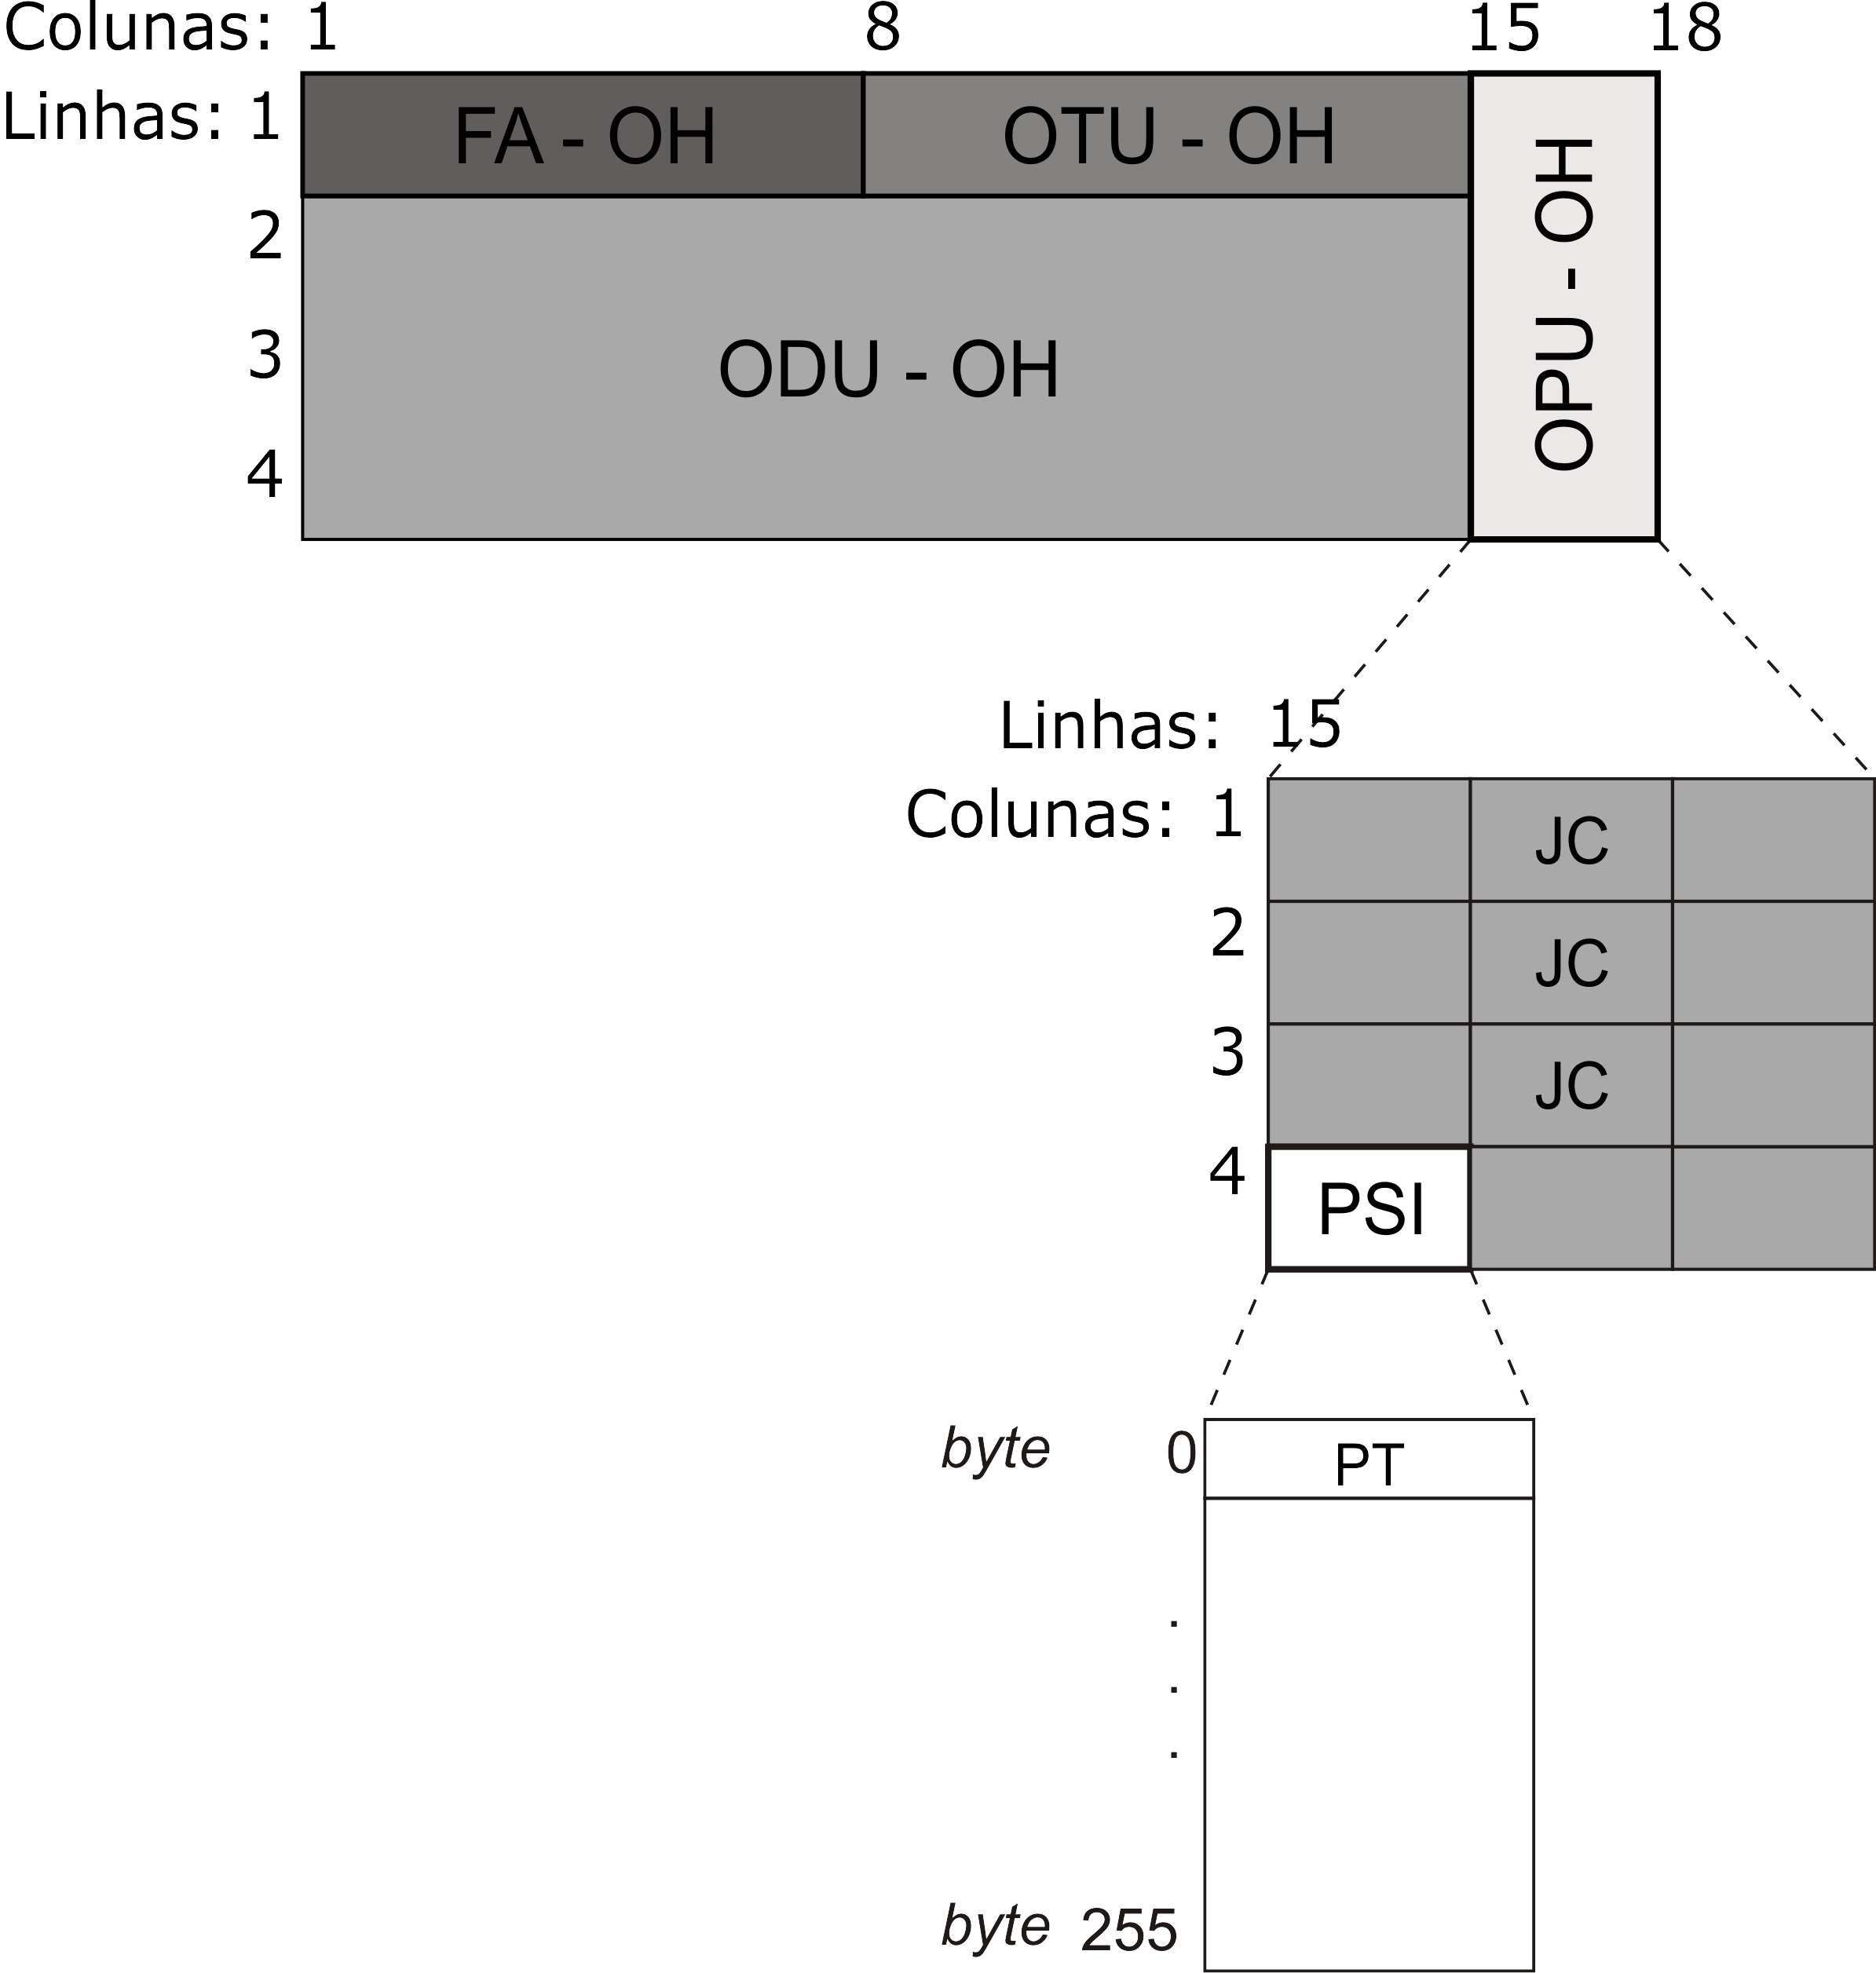
\includegraphics[scale=.7]{./cap3/otn_opu_oh.png}
 % sistema_fec.png: 2786x729 pixel, 600dpi, 11.79x3.09 cm, bb=
 \caption{Estrutura do cabe�alho da unidade de carga �til do canal �tico.}
 \label{fig:otn_opu_oh}
\end{figure}


O padr�o G.709 suporta tanto sinais com taxa de \textit{bit} constante (\ac{CBR} -- \ac{CBR}) como sinais baseados em pacotes ou c�lulas. Assim, para tratar o sinal cliente de forma transparente dentro da \ac{OTN} � necess�rio fazer o mapeamento da taxa deste sinal no OPU-OH. Isto � feito de forma diferente dependendo da taxa de transmiss�o do cliente em rela��o � taxa da interface \ac{OTU}$k$, caso haja assincronia entre os \textit{clocks} das interfaces cliente e \ac{OTU}$k$. Neste caso, para fazer o mapeamento s�o utilizados os subcampos \ac{JC} que compensam a diferen�a entre os \textit{clocks}. No caso de sinais s�ncronos, os campos \ac{JC} s�o preenchidos com zeros.

O tipo de carga �til transportada no quadro da \ac{OTN} � identificado pelo campo \ac{PT}. A Tabela~\ref{tab:payload_type} apresenta alguns dos tipos de sinais suportados~\cite{Gorshe2009}, para mais detalhes sobre cada tipo de \textit{payload} recomenda-se ler a documenta��o do G.709~\cite{G709}.

\begin{table}[H]
\begin{center}
\begin{threeparttable}
\caption{Tipos de sinais suportados pelo padr�o ITU-T G.709}
\label{tab:payload_type}
\begin{tabular}{ll} \hline
C�digo (Hex) & Tipo de \textit{payload}\\ \hline
01 & Mapeamento experimental\\ 
02 & \ac{CBR} ass�ncrono\\ 
03 & \ac{CBR} s�ncrono\\ 
04 & \ac{ATM}\\ 
05 & \ac{GFP}\\ 
06 & \ac{VCAT}\\ 
07 & \textit{Ethernet} 1000BASE-X dentro do ODU0\\ 
08 & \ac{FC1200} dentro do ODU2e\\ 
09 & Mapeamento GFP dentro do \textit{payload} do OPU2\\ 
10 & \textit{Bit stream} com mapeamento de \textit{clock} em octetos\\ 
11 & \textit{Bit stream} sem mapeamento de \textit{clock} em octetos\\  
20 & estrutura de multiplexa��o do ODU\\ 
21 & estrutura tribut�ria para $1,25~Gbps$ em OPU2 ou OPU3 \\ 
80-8F & c�digos reservados para uso propriet�rio\\ 
\hline
\end{tabular}
\end{threeparttable}
\end{center}
\end{table}

\section{Principais Falhas e Alarmes}
\label{sec:alarmes_g709}

A principal indica��o de falhas da \ac{OTN} est� relacionada ao alinhamento do sinal, ou seja, quando o in�cio e/ou fim do quadro n�o � identificado. Os \textit{bytes} da �rea de alinhamento do sinal podem indicar condi��es como: \ac{OOF}, \ac{OOM}, \ac{LOF} e \ac{LOM}. Quando os  \textit{bytes} campo \ac{FAS} n�o s�o reconhecidos durante cinco quadros consecutivos ou persiste durante $3~ms$, o protocolo G.709 alerta sobre eventos de \ac{OOF} e \ac{LOF}, respectivamente. Al�m disso, os eventos de \ac{OOM} ou \ac{LOM} acontecem quanto h� falhas no reconhecimento de cinco quadros consecutivos ou durante $3~ms$ com erros no campo \ac{MFAS}, respectivamente. 

Outros indicadores de erros que correspondem � qualidade de transmiss�o digital est�o presentes nos subcampos \ac{BIP-8}, \ac{BEI}, \ac{BDI} dos campos \acl{SM} no OTU-OH, e nos campos \acl{PM} e \ac{TCM}$i$ do ODU-OH. O \ac{BIP-8} armazena \textit{bytes} de paridade que s�o calculados sobre a carga �til e o OPU-OH. O c�lculo do \ac{BIP-8} � realizado antes de ser aplicada a \ac{FEC} na dire��o de transmiss�o e verificado depois da \ac{FEC} na dire��o de recep��o. Os valores calculados do \ac{BIP-8} s�o inseridos no segundo quadro posterior ao utilizado para o c�lculo. A capacidade de detec��o de erros de paridade � de 8 bits por 15.$240~bytes$, o que corresponde a uma taxa erros de bit m�xima de $6,56$x$10^{-5}$. O campo \ac{BEI} � utilizado no sentido inverso, ou seja, para informar ao transmissor que erros de \ac{BIP-8} foram encontrados nos quadros recebidos. O campo \ac{BDI} � usado para indicar \textit{upstream} que  h�  um  problema  de  conectividade,  continuidade  ou  um  sinal  de  manuten��o ativo~\cite{Barlow2004, G709}. 

\section{O C�digo Corretor de Erros (FEC)}

O padr�o G.709 suporta a corre��o de erros a partir do campo \ac{FEC} contido no quadro da OTN (Figura~\ref{fig:otn_quadro}). A \ac{FEC} reduz o n�mero de erros transmitidos devido ao ru�do e fen�menos �ticos que ocorrem na fibra operando em altas taxas de transmiss�o (vide Sess�o~\ref{sec:ro_impairments}). Assim, o G.709 permite que o sinal seja transmitido por grandes dist�ncias entre repetidores �ticos sem a necessidade de regenera��o. Isso torna a FEC um importante recurso da OTN. O c�lculo � definido a partir de um esquema de $16~bytes$ entrela�ados utilizando o algoritmo \ac{RS}. Tal algoritmo usa $1024~bytes$ de informa��o de verifica��o por quadro ODU. Al�m disso, v�rios esquemas de propriet�rios de \ac{FEC} tamb�m s�o permitidos e s�o amplamente utilizados~\cite{Walker2007}. 

O algoritmo \acl{RS} empregado pelo padr�o G.709 melhora a rela��o sinal ru�do (\aclu{SNR} -- \ac{SNR}) em at� $6.2~dB$ para sistemas que exigem \ac{BER} de at� $10^{-15}$~\cite{Walker2007}. A melhoria da \ac{SNR} fornecida pela \ac{FEC} � chamada de ganho de codifica��o, em que os benef�cios por tr�s deste ganho, al�m do alcance do sinal, s�o: (\textit{i}) par�metros menos restritos para pot�ncia de sa�da, raz�o de extin��o, presen�a de ru�do e filtros isolantes, reduzindo o custo dos componentes do enlace �tico; (\textit{ii}) aumentar o n�mero de canais em sistemas \ac{WDM}, os quais est�o limitados pela pot�ncia de sa�da dos amplificadores e (\textit{iii}) consolida��o das redes totalmente �ticas, pois permite que o sinal atravesse transparentemente um maior n�meros de componentes �ticos (\acp{OXC} e \acp{OADM}) sem a necessidade de regenera��o, visto que tais componentes adicionam uma quantidade significante de degrada��es do sinal~\cite{Walker2007}.

O \acl{RS} � denominado como \ac{RS}$(n,k)$. Nesse algoritmo s�o utilizados $n$ s�mbolos por palavra-c�digo, mas somente uma parte $k$ desses $n$ s�mbolos cont�m a informa��o propriamente dita e cada s�mbolo deve possui um n�mero $s$ de bits. Desta forma, uma palavra-c�digo consiste de uma parte de dados que cont�m a informa��o e outra parte de s�mbolos de checagem ou paridade. S�o justamente os s�mbolos de paridade que permitem que o algoritmo possa corrigir e recuperar a informa��o em sinais com erros detectados. A {FEC} empregada pelo G.709, faz uso do c�digo \ac{RS}(255, 239). A Figura~\ref{fig:sistema_fec} apresenta um diagrama de blocos de aplica��o da FEC baseada no algoritmo \ac{RS} em um sistema b�sico de comunica��o.


\begin{figure}[H]
 \centering
 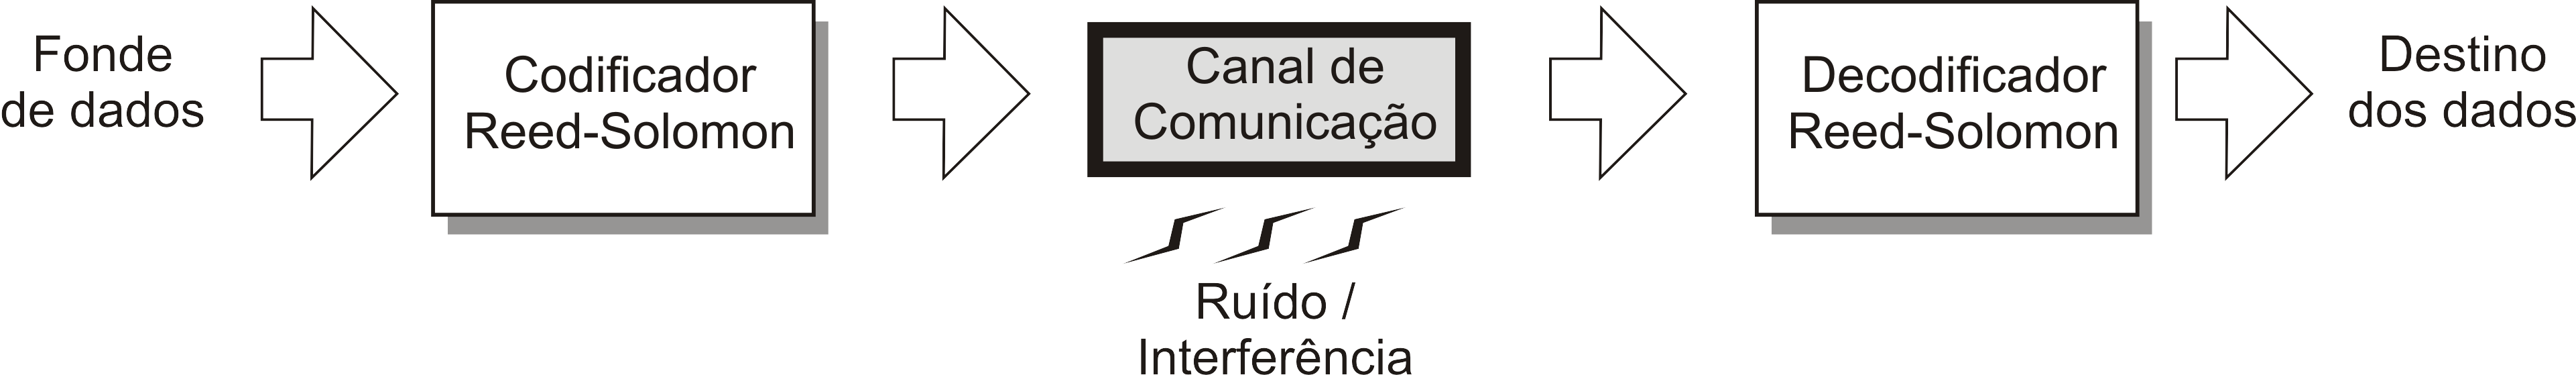
\includegraphics[scale=1]{./cap3/sistema_fec.png}
 % sistema_fec.png: 2786x729 pixel, 600dpi, 11.79x3.09 cm, bb=
 \caption{Diagrama de blocos de aplica��o da FEC no sistema.}
 \label{fig:sistema_fec}
\end{figure}


O decodificador RS pode corrigir at� $t$ s�mbolos que contenham erros na palavra-c�digo, em que $2t=n-k$. No caso do c�digo RS(255 ,239), tem-se: $2t = n-k = 255-239 = 16 $, logo o decodificador pode corrigir $t = 8$ s�mbolos por palavra. Como o c�digo do RS utiliza os s�mbolos das palavra-c�digo, assim ele tem o mesmo desempenho para corrigir um s�mbolo com todos os \textit{bits} errados que um s�mbolo com apenas um \textit{bit} errado. A Tabela~\ref{tab:parametros_fec} apresenta os par�metros do RS(255,239).

\begin{table}[H]
\begin{center}
\begin{threeparttable}
\caption{Par�metros do algoritmo \acl{RS}(255,239).}
\label{tab:parametros_fec}
\begin{tabular}{lcl} \hline
\textbf{Descri��o} & s�mbolo & valor \\ \hline
Tamanho do s�mbolo & $s$ & $8~bits$\\ 
N� de s�mbolos por palavra-c�digo & $n$ & $255~bytes$\\ 
S�mbolos de informa��o por palavra-c�digo  & $k$ & $239~bytes$	\\ 
\hline
\end{tabular}
\end{threeparttable}
\end{center}
\end{table}

A \ac{FEC} ainda entrela�a a informa��o, e assim, permite corrigir erros em rajada. Com o entrela�amento,  erros encontrados em um \textit{stream} de \textit{bits} s�o compartilhados por diversas palavras-c�digo, o que torna o algoritmo mais eficiente. Assim, o ganho de codifica��o � melhorado por unir o entrela�amento da informa��o e a efici�ncia do algoritmo \ac{RS}(255, 239), permitindo que at� 128 \textit{bytes} consecutivos recebidos com erros sejam corrigidos~\cite{G709, G975}.

\chapter{Plano de Controle GMPLS}
\label{cap:gmpls}

O \ac{IETF} especificou um novo plano de controle chamado \ac{GMPLS}~\cite{Farrel2006, Bernstein2003}, que � capaz de operar com diferentes tecnologias de transporte, tais como: pacotes/c�lulas \ac{IP}/\ac{ATM} (\aclu{PSC} -- \ac{PSC}), dados na camada de enlace (\aclu{L2SC} -- \ac{L2SC}), quadros de tempo (\ac{TDM}), fibras �ticas (\aclu{FSC} -- \ac{FSC}) e comprimentos de onda (\ac{LSC} -- \ac{LSC}). O \ac{GMPLS} consiste em uma generaliza��o do conjunto de protocolos do \ac{MPLS}~\cite{rfc3031}, seu precursor, pois este comuta apenas pacotes \ac{IP} e \ac{L2SC}. A capacidade de comuta��o por r�tulo consiste em atribuir um identificador referente a uma categoria ou classe. Ent�o, os dados podem ser encaminhados de um roteador para outro simplesmente verificando este identificador. 

Nas redes GMPLS, os roteadores respons�veis pela transmiss�o de dados s�o denominados \acp{LSR} e o caminho de dados entre os \acp{LSR} origem e destino � chamado de \ac{LSP}. Neste trabalho, os \acp{LSP} estabelecidos pelo plano de controle \ac{GMPLS} ser�o formados por caminhos comutados por comprimentos de onda, tamb�m chamados de caminhos �ticos conforme apresentado nos Cap�tulos~\ref{cap:rede_otica} e~\ref{cap:g709}. 

O \ac{GMPLS} permite que os \acp{LSP} sejam organizados como uma hierarquia formada de acordo com o tipo de comuta��o. Na Figura~\ref{fig:hierarquiaLSPs} pode-se observar a forma��o de uma hierarquia em que um \ac{LSP} de maior ordem (fibra) � capaz de transmitir diversos comprimentos de onda (\ac{LSC}), esse por sua vez, pode transportar \acp{LSP} baseados na divis�o de tempo (\ac{TDM}), enquanto que em cada quadro de tempo s�o multiplexados \acp{LSP} de pacotes (\ac{PSC}).

\begin{figure}[H]
	\centering
		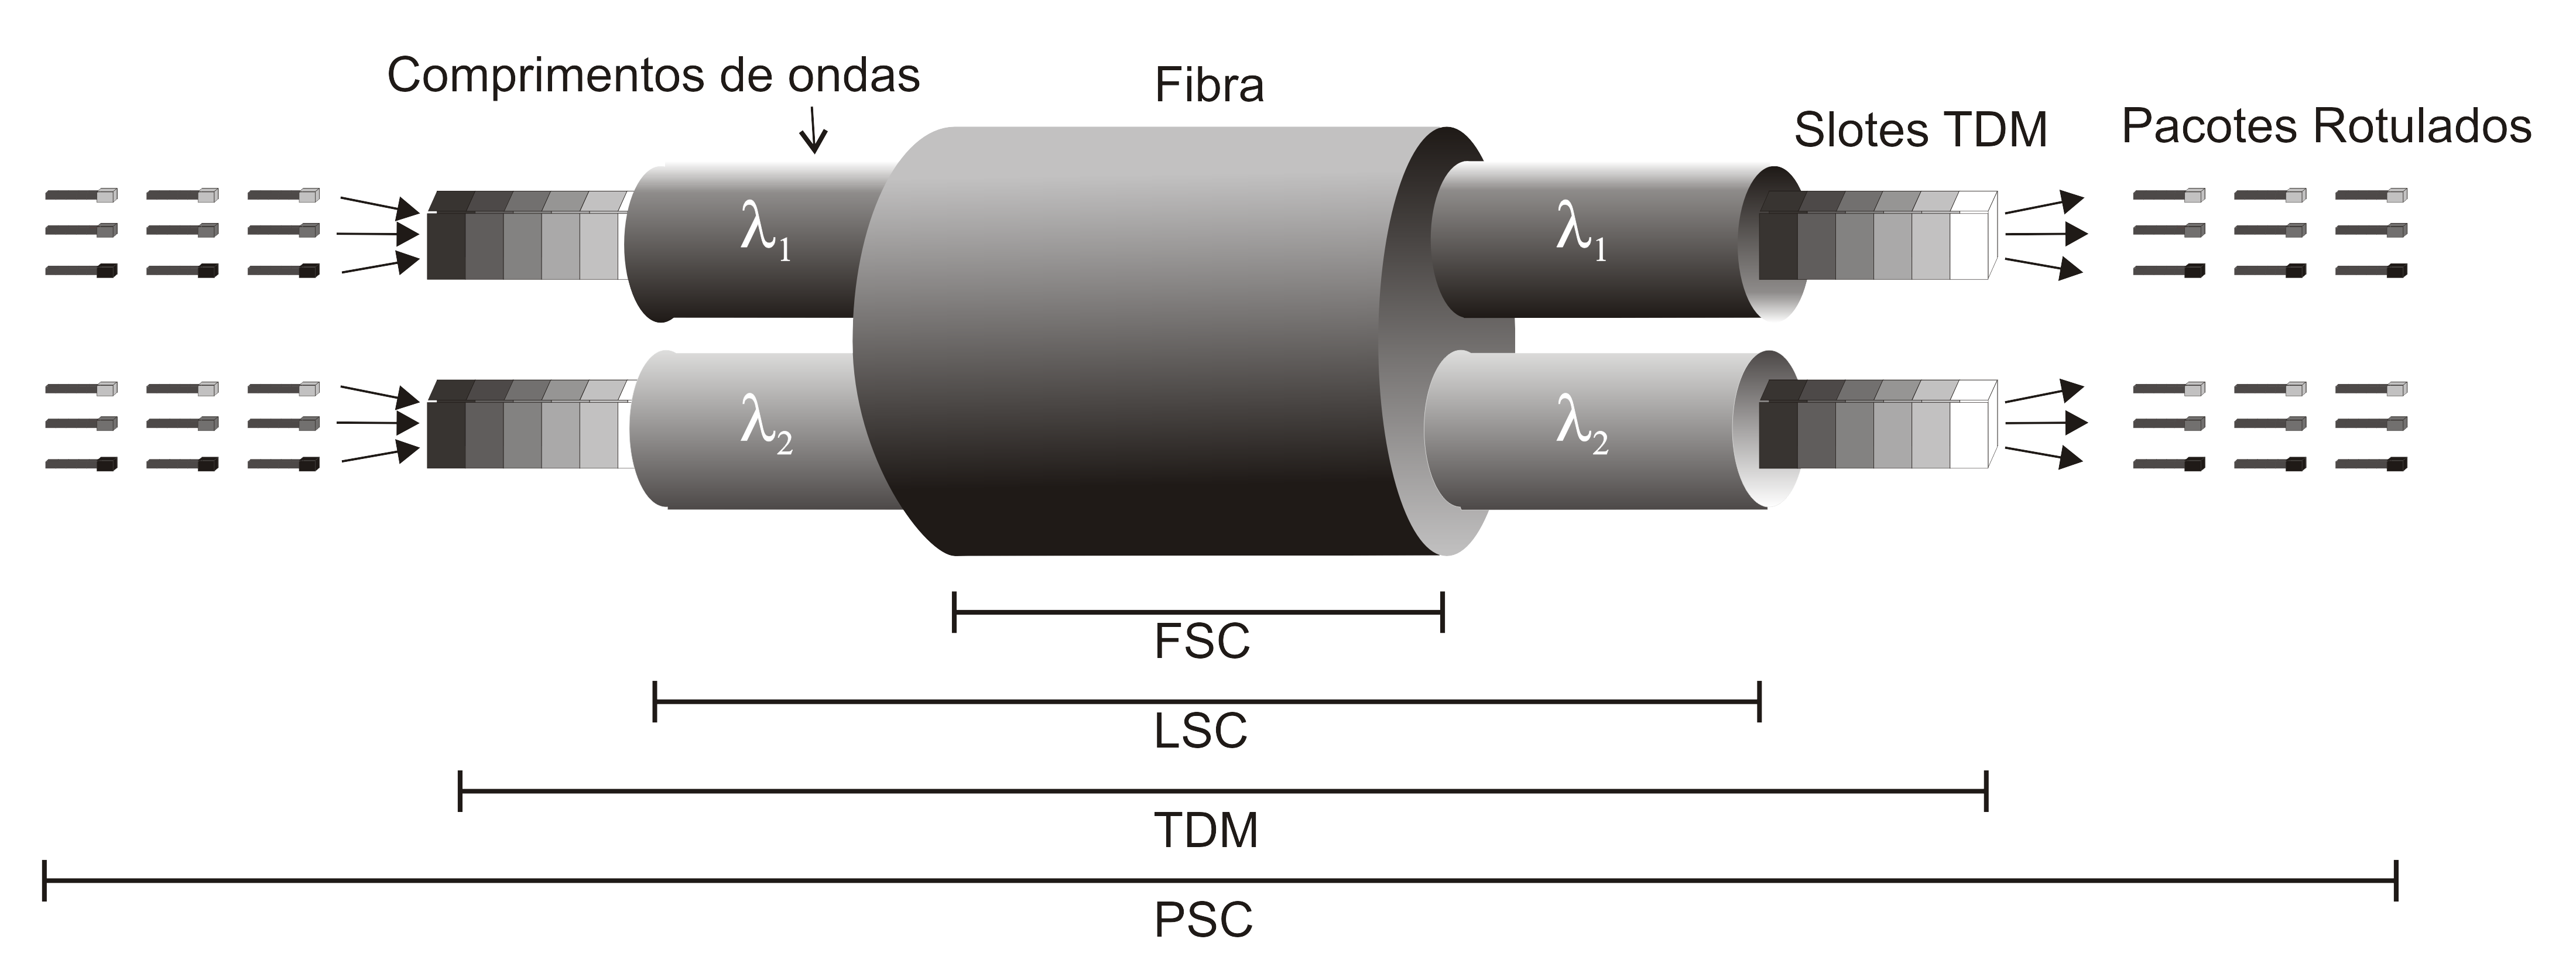
\includegraphics[scale=.8]{cap4/hierarquiaLSPs2.png}
	\caption{Hierarquia de LSPs utilizando diferentes capacidades de multiplexa��o.}
	\label{fig:hierarquiaLSPs}
\end{figure}

A utiliza��o de uma hierarquia de \ac{LSP} contendo todas as tecnologias da Figura \ref{fig:hierarquiaLSPs} traz uma importante desvantagem: o \textit{overhead} de processamento necess�rio para analisar a informa��o que � transmitida e/ou recebida. Por exemplo, quando um pacote IP � enviado, os cabe�alhos de cada protocolo relativo �s tecnologias de transmiss�o s�o inseridos no pacote, que ao ser recebido tem seus os cabe�alhos analisados e removidos. O \textit{overhead} gerado pelo processamento de inser��o, an�lise e remo��o de cabe�alhos causa atrasos na execu��o de tarefas do plano de controle. Tais atrasos podem ser evitados ao utilizar uma pilha de protocolos mais compacta. O \ac{GMPLS} traz uma boa solu��o para este problema ao permitir que \ac{LSP} de pacotes sejam diretamente multiplexados na rede �tica. Isto significa dizer que a camada de rede IP pode interagir diretamente com a camada fot�nica. 

� comum referir-se �s camadas superiores, por exemplo \ac{IP}, \ac{ATM}, \ac{SONET}/\ac{SDH}, como clientes da camada �tica. O n�vel de intera��o entre as camadas cliente e �tica � determinado pelo modelo de plano de controle adotado. Dentre eles pode-se citar:

\begin{itemize}
	\item \textbf{Modelo integrado (\textit{peer}):} Neste modelo, as camadas cliente e �tica possuem um plano de controle em comum e as informa��es sobre rota, topologia e restri��es das duas camadas s�o compartilhadas, desta forma os roteadores da rede podem determinar o caminho fim-a-fim, inclusive o caminho �tico;
	\item \textbf{Modelo de sobreposi��o de camadas (\textit{overlay}):} H� dom�nios administrativos distintos, ou seja, h� um software de plano de controle diferente para tratar cada camada, portanto nenhuma informa��o de topologia nem de roteamento � trocada, deixando-as totalmente isoladas;
	\item \textbf{Modelo expandido (\textit{augmented}):} Esta � uma abordagem h�brida dos modelos anteriores. H� um n�vel controlado de troca de informa��es entre as camadas. Os roteadores possuem um resumo de informa��es sobre rotas e topologia �tica, mas ainda s�o mantidos os softwares de plano de controle separados.
\end{itemize}

A arquitetura do \ac{GMPLS} permite que a troca de informa��es entre as camadas seja manipulada livremente, assim a decis�o do modelo a ser implementado fica sob a responsabilidade do projetista da rede, que tamb�m dever� escolher como as informa��es da rede estar�o distribu�das. Estas informa��es podem estar armazenadas da seguinte forma:

\begin{itemize}
	\item \textbf{Centralizada:} Um controlador central tem conhecimento da rede por inteiro, ou seja, possui um �nico banco de dados que cont�m o estado global da rede. Assim, ele pode atender ou recusar um pedido de caminho �tico de imediato;
	\item \textbf{Distribu�da:} H� um controlador em cada n� e as informa��es de estado encontram-se nos bancos de dados contidos nos n�s. Ao receber uma requisi��o, � necess�rio que cada controlador verifique localmente se � poss�vel atend�-la. Neste caso faz-se necess�rio alguma forma de dissemina��o de informa��es.
\end{itemize}

\section{Protocolo GMPLS RSVP-TE}
\label{sec:rsvp}

A primeira vers�o do \ac{RSVP}~\cite{rfc2205} foi especificada somente como um protocolo de reserva de recursos, que fazia parte de uma arquitetura de Qualidade de Servi�o -- \ac{QoS} montada para atender os requisitos de algumas aplica��es~\cite{Gozdecki2003}, tais como voz sobre \ac{IP} -- \ac{VoIP}, \textit{streams} multim�dia sob demanda e v�deo-confer�ncia. Devido � sua extensibilidade e flexibilidade, come�ou a ser utilizado como protocolo de sinaliza��o do \ac{MPLS}, sendo respons�vel por transportar informa��es para o estabelecimento de \acp{LSP}. Posteriormente, ele foi aperfei�oado para fazer engenharia de tr�fego, provendo mecanismos de r�pido rerroteamento e controle de falhas~\cite{rfc2702,rfc3209}, passando ent�o a ser chamado \ac{RSVP-TE}. O \ac{RSVP-TE} introduziu o conceito de t�neis comutados por r�tulos (\textit{LSP tunnels}), em que um t�nel pode ser entendido como um ``tubo'' que conecta uma origem a um destino, sendo chamados de \textit{ingresso} e \textit{egresso}, respectivamente. Os t�neis \acp{LSP} permitem executar pol�ticas de otimiza��o, isto �, roteamento autom�tico ou manual (em caso de falha ou congestionamento ou a fim de evitar a passagem pelo n�cleo da rede)~\cite{rfc3209}.

Com o surgimento do \ac{GMPLS}, o \ac{RSVP-TE} recebeu v�rias atualiza��es, tais como~\cite{rfc3471, rfc3473}: (\textit{i}) possibilidade de estabelecer \ac{LSP} bidirecionais; (\textit{ii}) sugest�o de r�tulo pela origem; (\textit{iii}) novos objetos para notifica��o de falhas e (\textit{iv}) novos mecanismos de prote��o e restaura��o. Entretanto, n�o houve mudan�as nos procedimentos de estabelecimento, manuten��o e remo��o de conex�es, apenas foram criados novos tipos de mensagens e objetos de dados, que aprimoraram as funcionalidades do protocolo.

\begin{figure}[H]
	\centering
		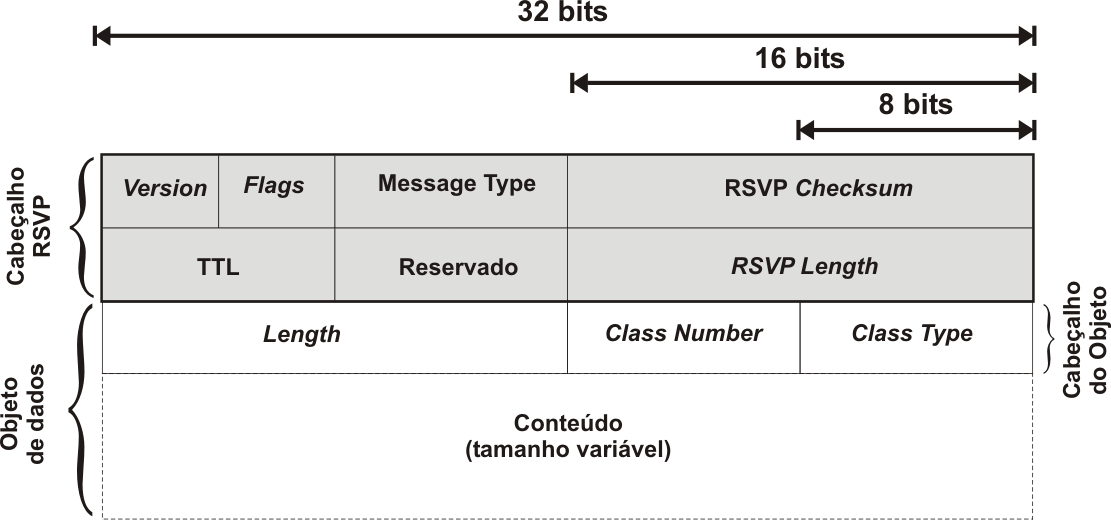
\includegraphics{cap4/cabecalhoRSVP2.png}
	\caption{Estrutura do cabe�alho comum (\textit{Common Header}) e de objetos de dados (\textit{Object Header}) do protocolo RSVP.}
	\label{fig:cabecalhoRSVP}
\end{figure}

Os pacotes ou mensagens do protocolo \ac{RSVP} podem ser datagramas \ac{IP} puros, identificados pelo n�mero 46~\cite{ianaProtocolNumber}, ou podem ser encapsulados dentro do protocolo \ac{UDP}. As mensagens \ac{RSVP} possuem um cabe�alho comum (\textit{Common Header}), que atrav�s do campo \textit{MESSAGE TYPE} identifica o tipo de mensagem. Atualmente est�o padronizadas 15 diferentes tipos de mensagens que s�o utilizadas pelo plano de controle \ac{GMPLS}~\cite{Komolafe2007}. Cada uma delas pode transportar diferentes objetos em seu conte�do. Estes objetos tamb�m possuem um cabe�alho padr�o, onde o campo \textit{CLASS NUMBER} faz a distin��o entre eles. Al�m disso, foi feita a padroniza��o de 70 objetos de dados~\cite{Komolafe2007}. A institui��o \ac{IANA} � respons�vel pela coordena��o dos recursos associados aos protocolos da Internet. Em seu s�tio~\cite{ianaRSVP} � encontrado a lista com os tipos de mensagens e objetos do protocolo \ac{RSVP}. A Figura~\ref{fig:cabecalhoRSVP} ilustra os cabe�alhos utilizados por esse protocolo.

\subsection{Estabelecimento de LSPs}

 
Na fase de estabelecimento, uma s�rie de mensagens s�o trocadas entre n�s \ac{RSVP} de origem e destino. A mensagem \textit{PATH} � transmitida no sentido do destinat�rio e cont�m as informa��es do pedido de estabelecimento de um caminho comutado por r�tulo. Ela transporta os seguintes objetos, entre outros~\cite{rfc3209,rfc2210,rfc3473}: 
\begin{itemize}
	\item \textit{SESSION OBJECT}: cont�m o identificador para o \ac{LSP} e endere�o do destino, podendo ser dos tipos \ac{IPv4} ou \ac{IPv6};
	\item \textit{SENDER TEMPLATE OBJECT}: identifica a origem transportando o seu endere�o (\ac{IPv4} ou \ac{IPv6});
	\item \textit{SENDER TSPEC OBJECT}: utilizado para caracterizar o fluxo que ir� passar pelo \ac{LSP};
	\item \textit{GENERALIZED LABEL REQUEST OBJECT}: respons�vel por transportar os requisitos de comuta��o do \ac{LSP};
	\item \textit{RSVP HOP}: utilizado para registrar o n� anterior a cada passo dado pela mensagem.
\end{itemize}

\begin{figure}[H]
	\centering
		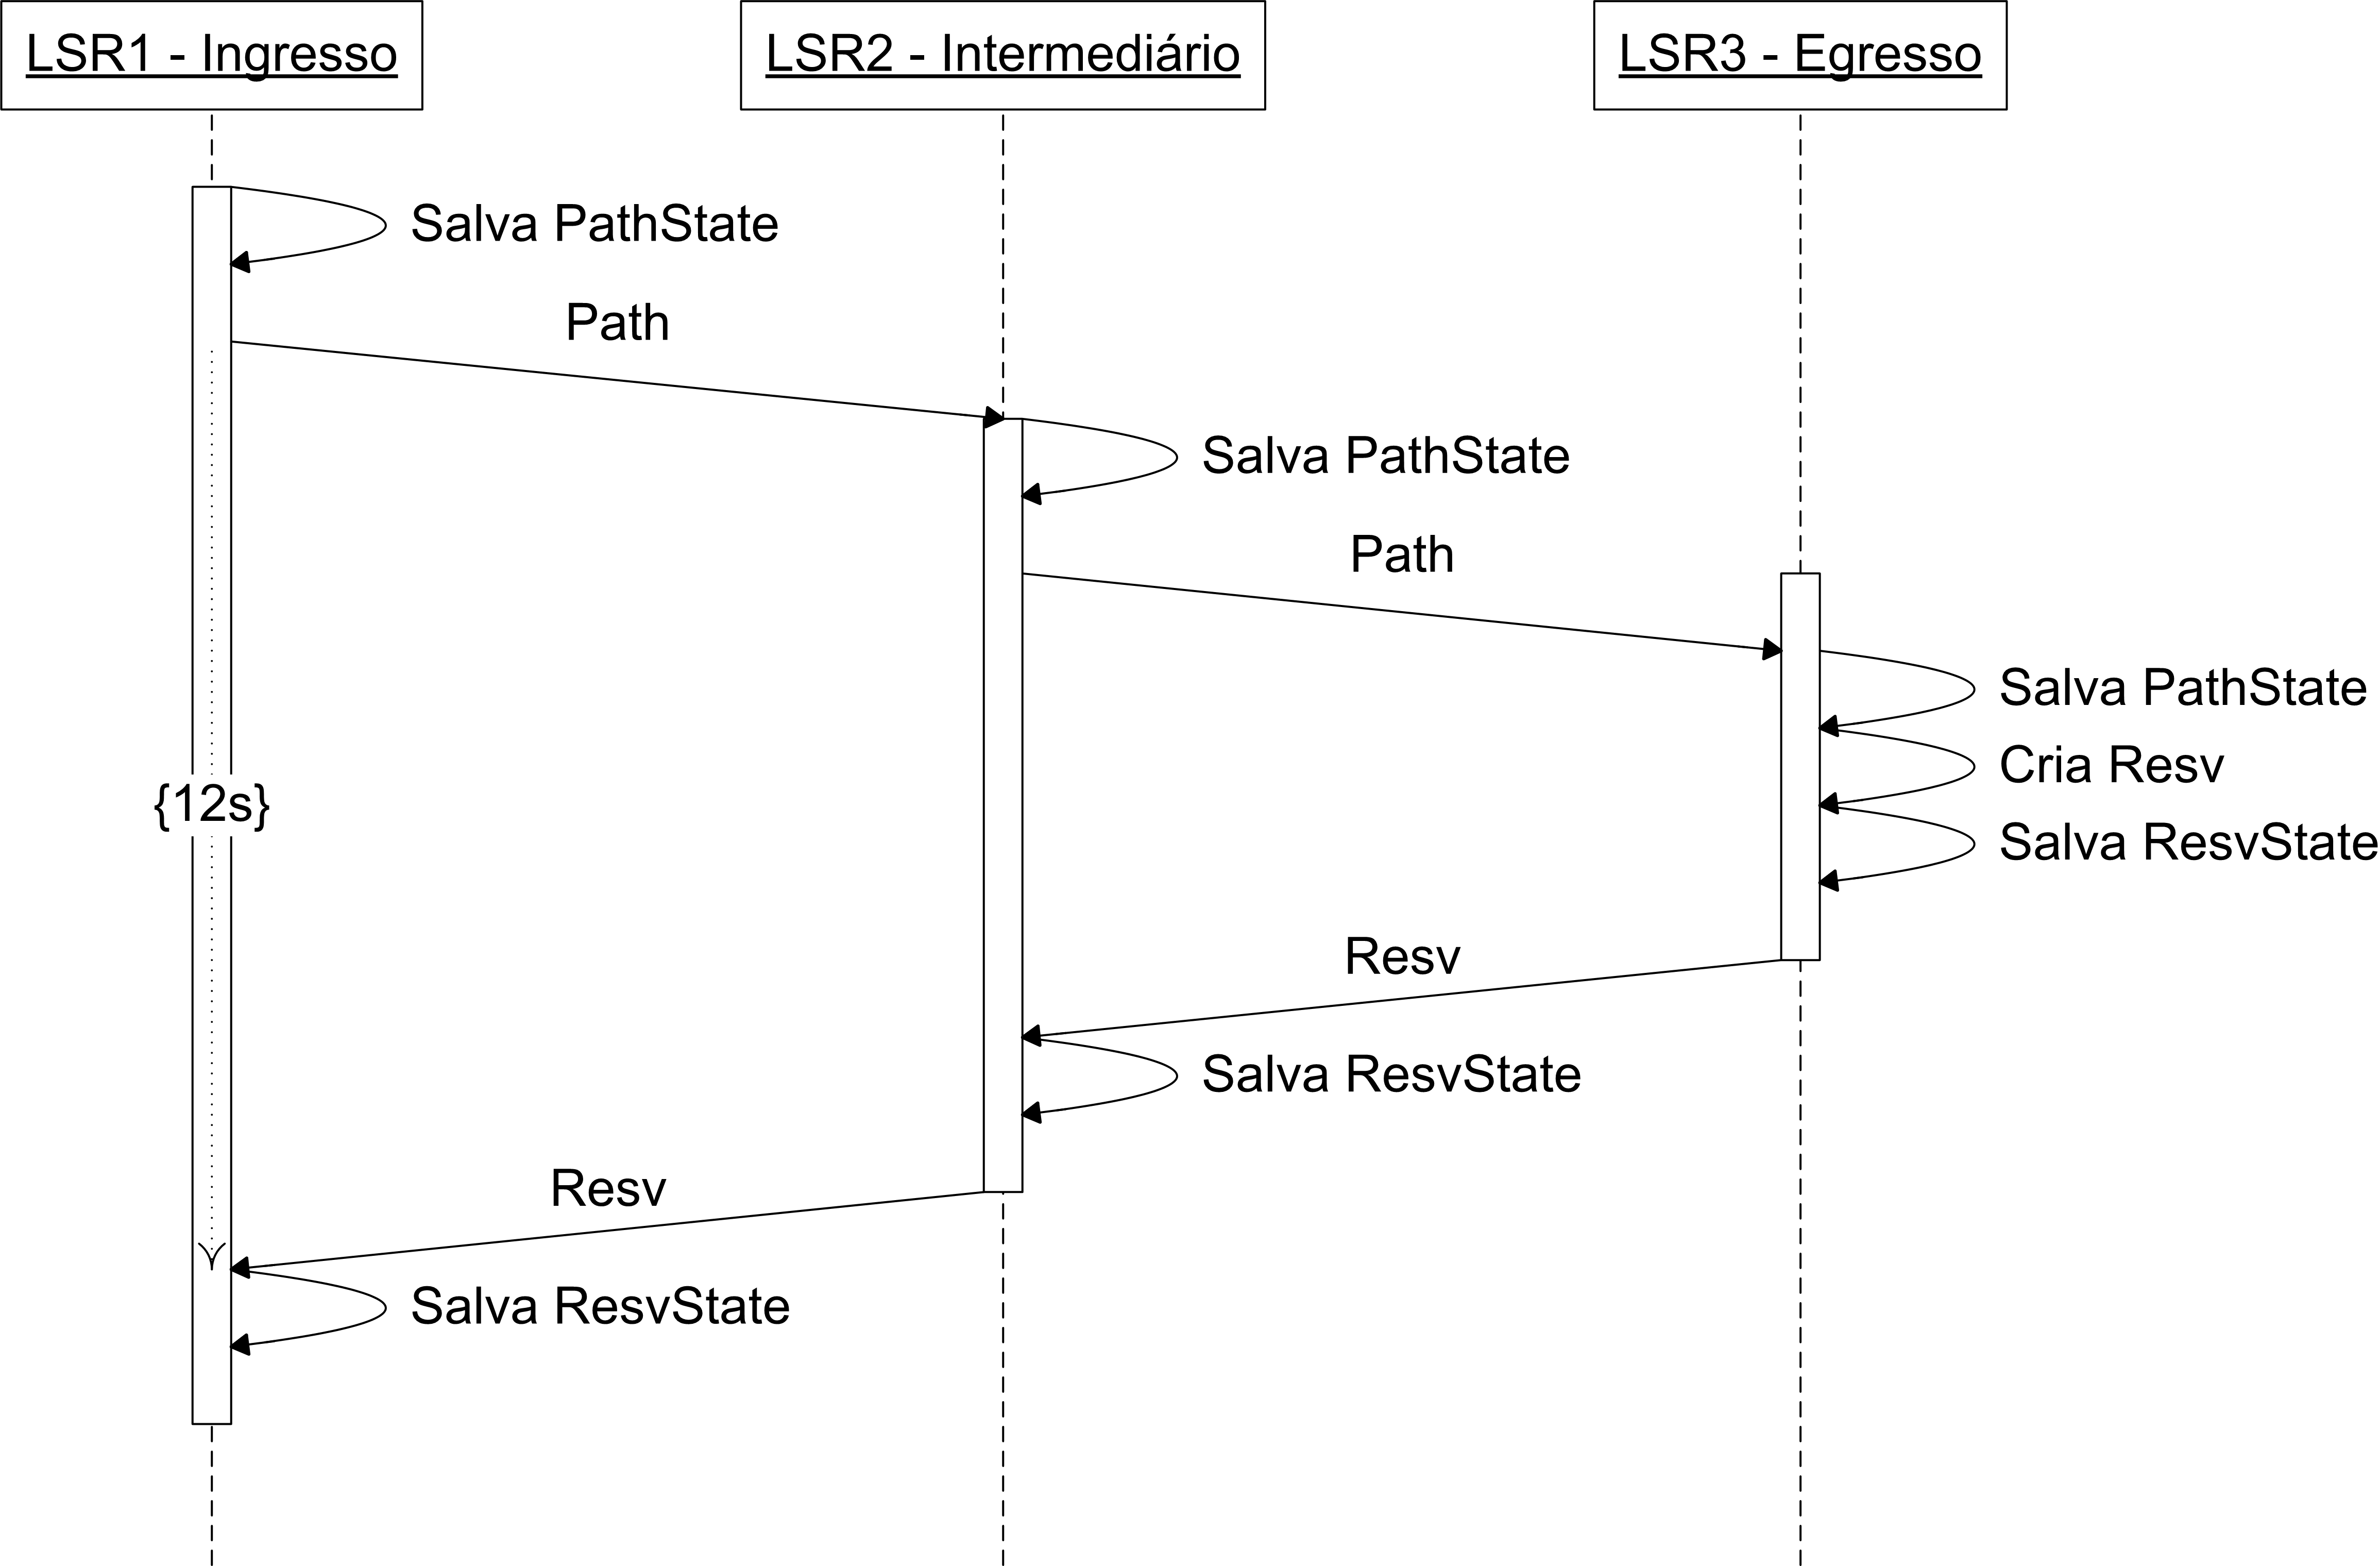
\includegraphics[scale=.6]{cap4/estabelecimento3.png}
	\caption{Diagrama de sequ�ncias da troca de mensagens RSVP necess�rias ao estabelecimento de um LSP.}
	\label{fig:gmpls_estabelecimento}
\end{figure}

A sinaliza��o para o estabelecimento das conex�es � ilustrada na Figura~\ref{fig:gmpls_estabelecimento}. Nessa fase, uma mensagem \textit{PATH} � enviada n� a n� at� alcan�ar o destino. A cada passagem por um n� intermedi�rio alguns procedimentos s�o executados, tais como: (\textit{i}) analisar os requisitos do \ac{LSP}; (\textit{ii}) atualizar o objeto \textit{RSVP HOP}; (\textit{iii}) gravar o estado da mensagem (\textit{PATHSTATE}) no n�. Al�m disso, a mensagem \textit{PATH} guarda as informa��es da rota que est� atravessando no objeto \textit{RECORD ROUTE OBJECT} cujo objetivo � evitar \textit{loops} na rede. O \ac{RSVP} d� suporte ao uso de rotas expl�citas atrav�s do objeto (\textit{EXPLICIT ROUTE OBJECT}) que pode ser adicionado a essa mensagem.

Quando a mensagem \textit{PATH} chega ao destino, o plano de controle escolhe um r�tulo (\textit{label}) relativo ao \ac{LSP} especificado no objeto \textit{GENERALIZED LABEL REQUEST}. A mensagem \textit{RESV}� criada com esse r�tulo e depois enviada no caminho de volta � origem (sentido \textit{upstream}) percorrendo exatamente o caminho contr�rio da mensagem \textit{PATH}. Para isto, ela faz uso da informa��o contida nos estados \textit{PATHSTATE} armazenados nos n�s em que mensagem \textit{PATH} atravessou. Ent�o, o plano de controle em cada n� insere o r�tulo recebido nas interfaces do roteador (entrada e sa�da) e grava as informa��es dos contidas nos objetos da mensagem \textit{RESV} no estado (\textit{RESVSTATE}). Se esta mensagem chegar � origem sem erros, imediatamente o \ac{LSP} ser� ativado e os dados j� poder�o ser transmitidos.

O protocolo \ac{RSVP-TE} permite que uma mensagem \textit{RESV} carregue diferentes r�tulos que s�o referentes a enlaces espec�ficos do caminho. Para isso, a mensagem \textit{RESV} deve conter um par de objetos \textit{FILTER SPEC} e \textit{GENERALIZED LABEL} para cada enlace espec�fico. O objeto \textit{GENERALIZED LABEL} transporta o r�tulo atribu�do ao enlace. Ele sempre deve ser precedido por um objeto \textit{FILTER SPEC}, cuja fun��o � identificar o roteador e a interface de destino do r�tulo. Os conte�dos das mensagens \textit{PATH} e \textit{RESV} podem ser visualizados nas Figuras \ref{fig:rsvppacketpath} e \ref{fig:rsvppacketresv}, respectivamente.

\begin{figure}[H]
	\centering
		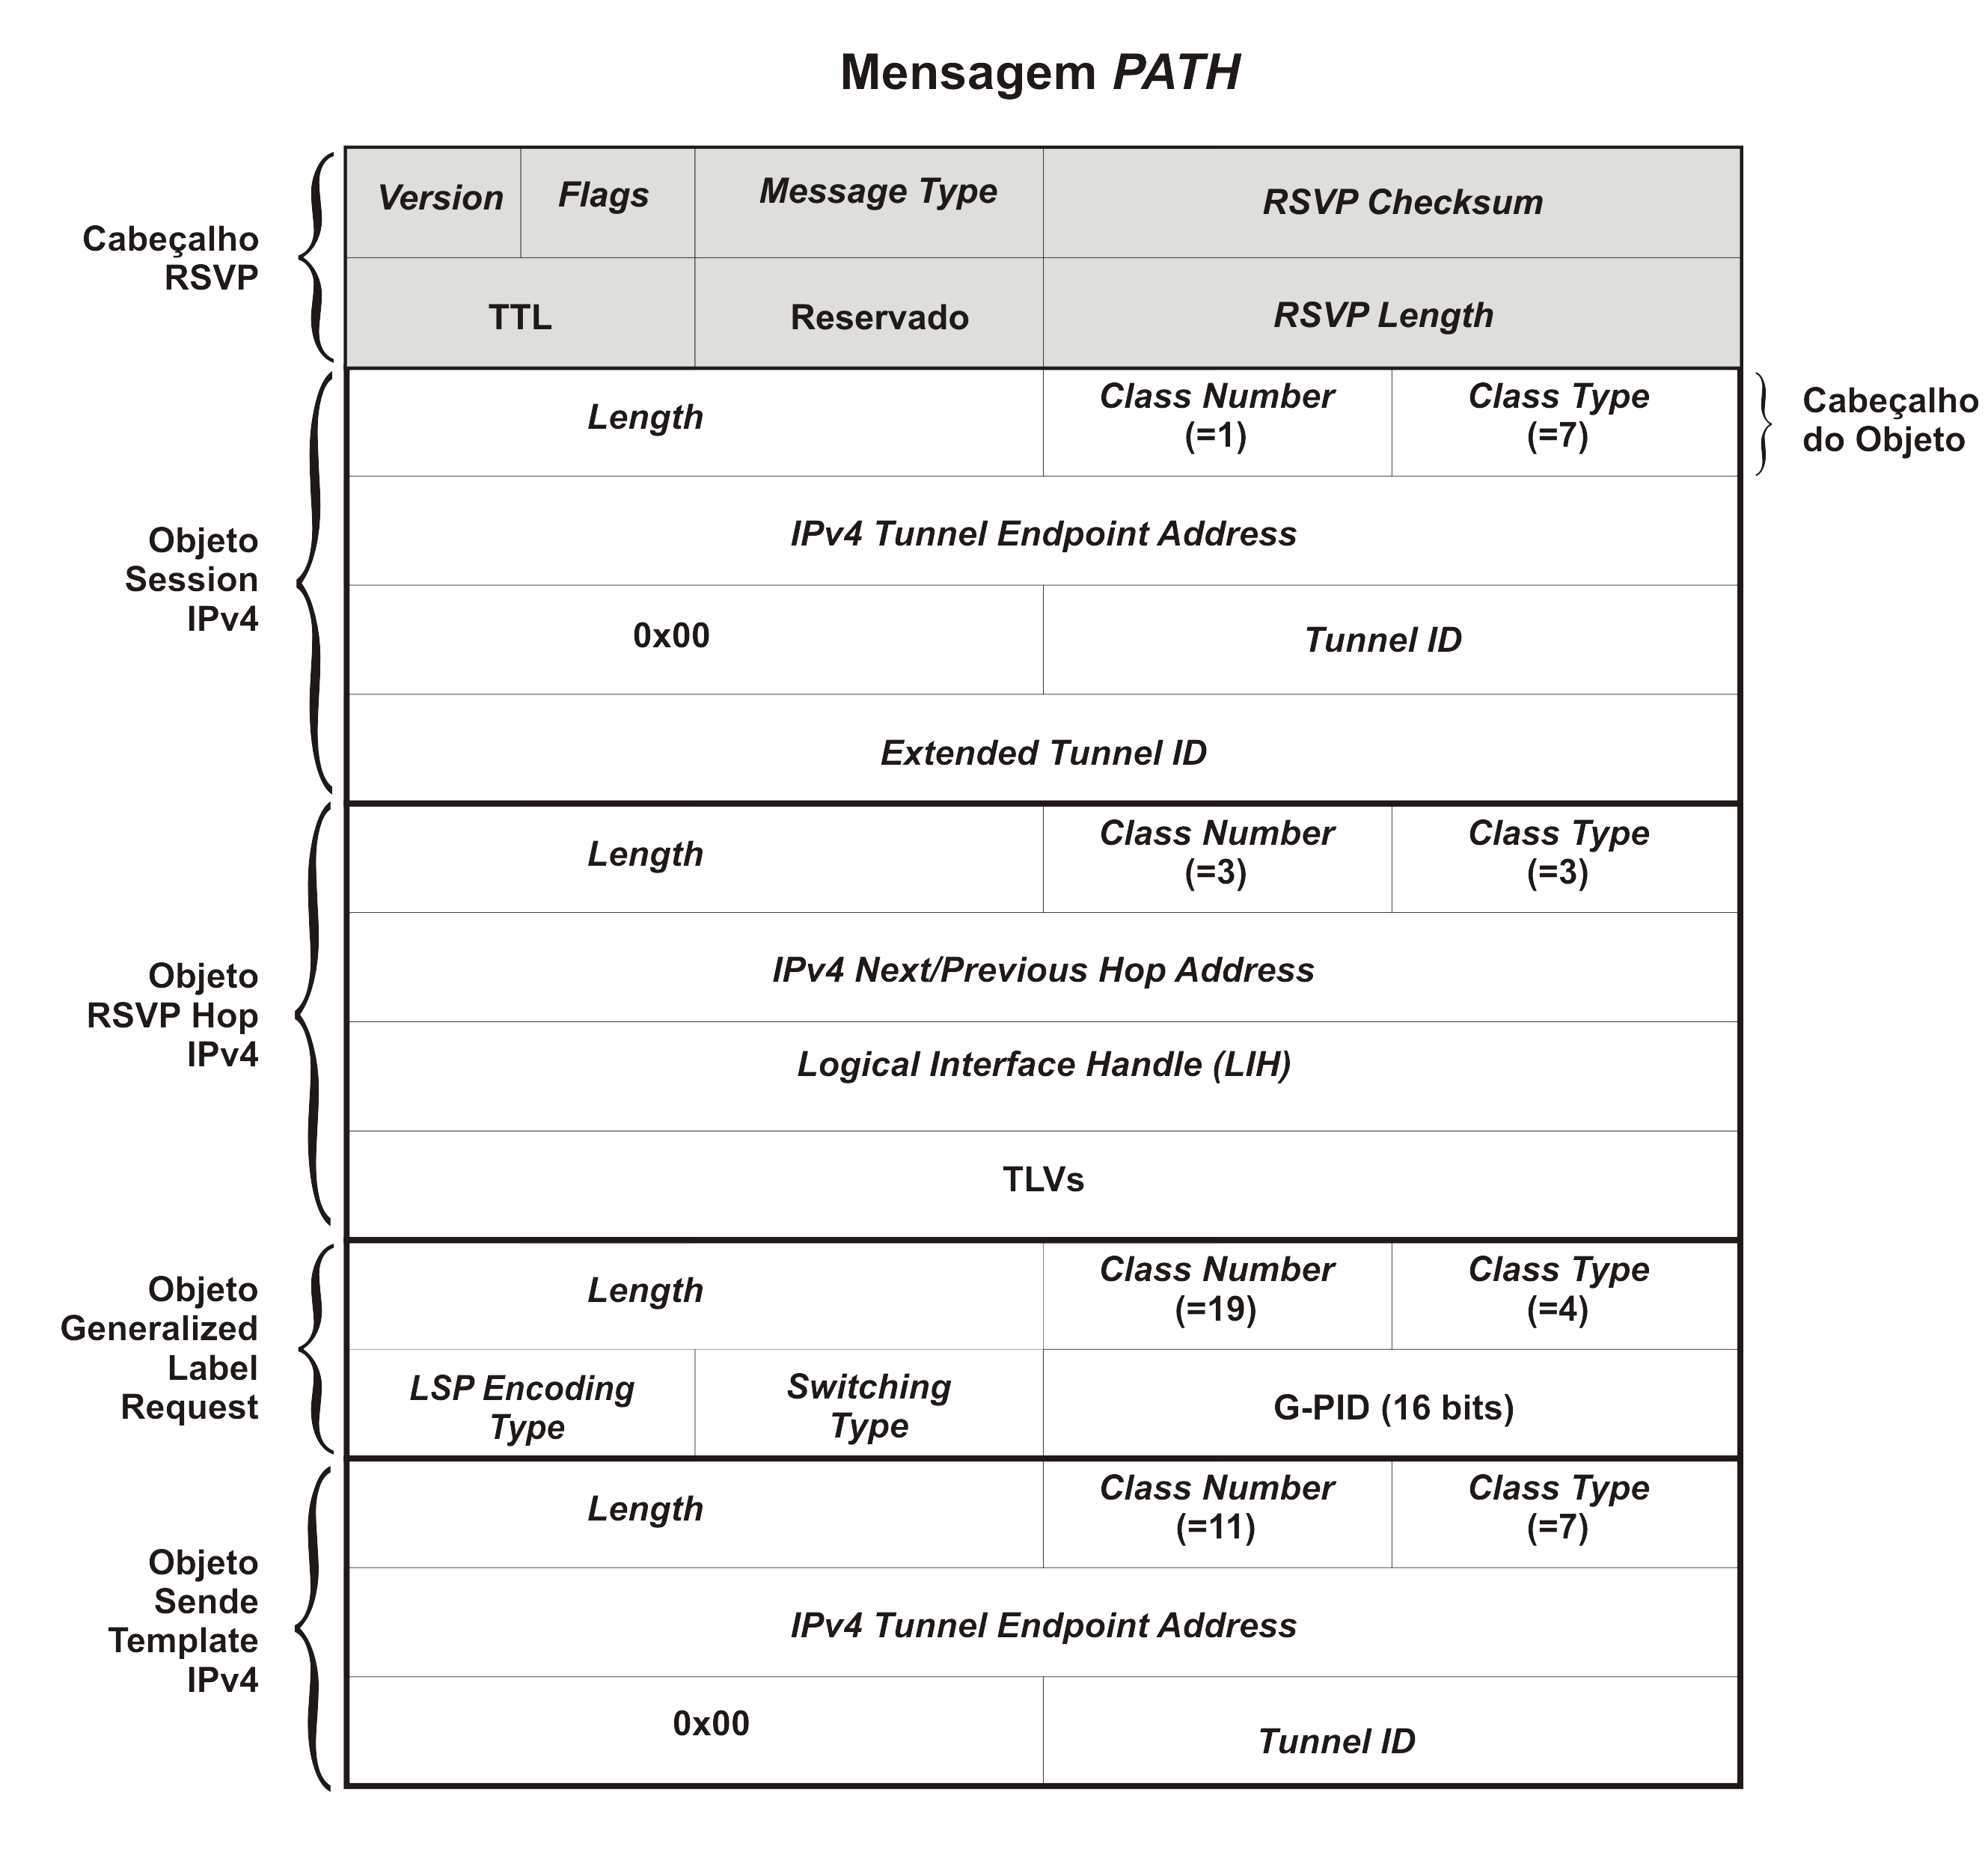
\includegraphics[scale=1]{cap4/rsvp-packet-path.png}
	\caption{Estrutura da mensagem \textit{PATH} do protocolo RSVP-TE.}
	\label{fig:rsvppacketpath}
\end{figure}

\begin{figure}[H]
	\centering
		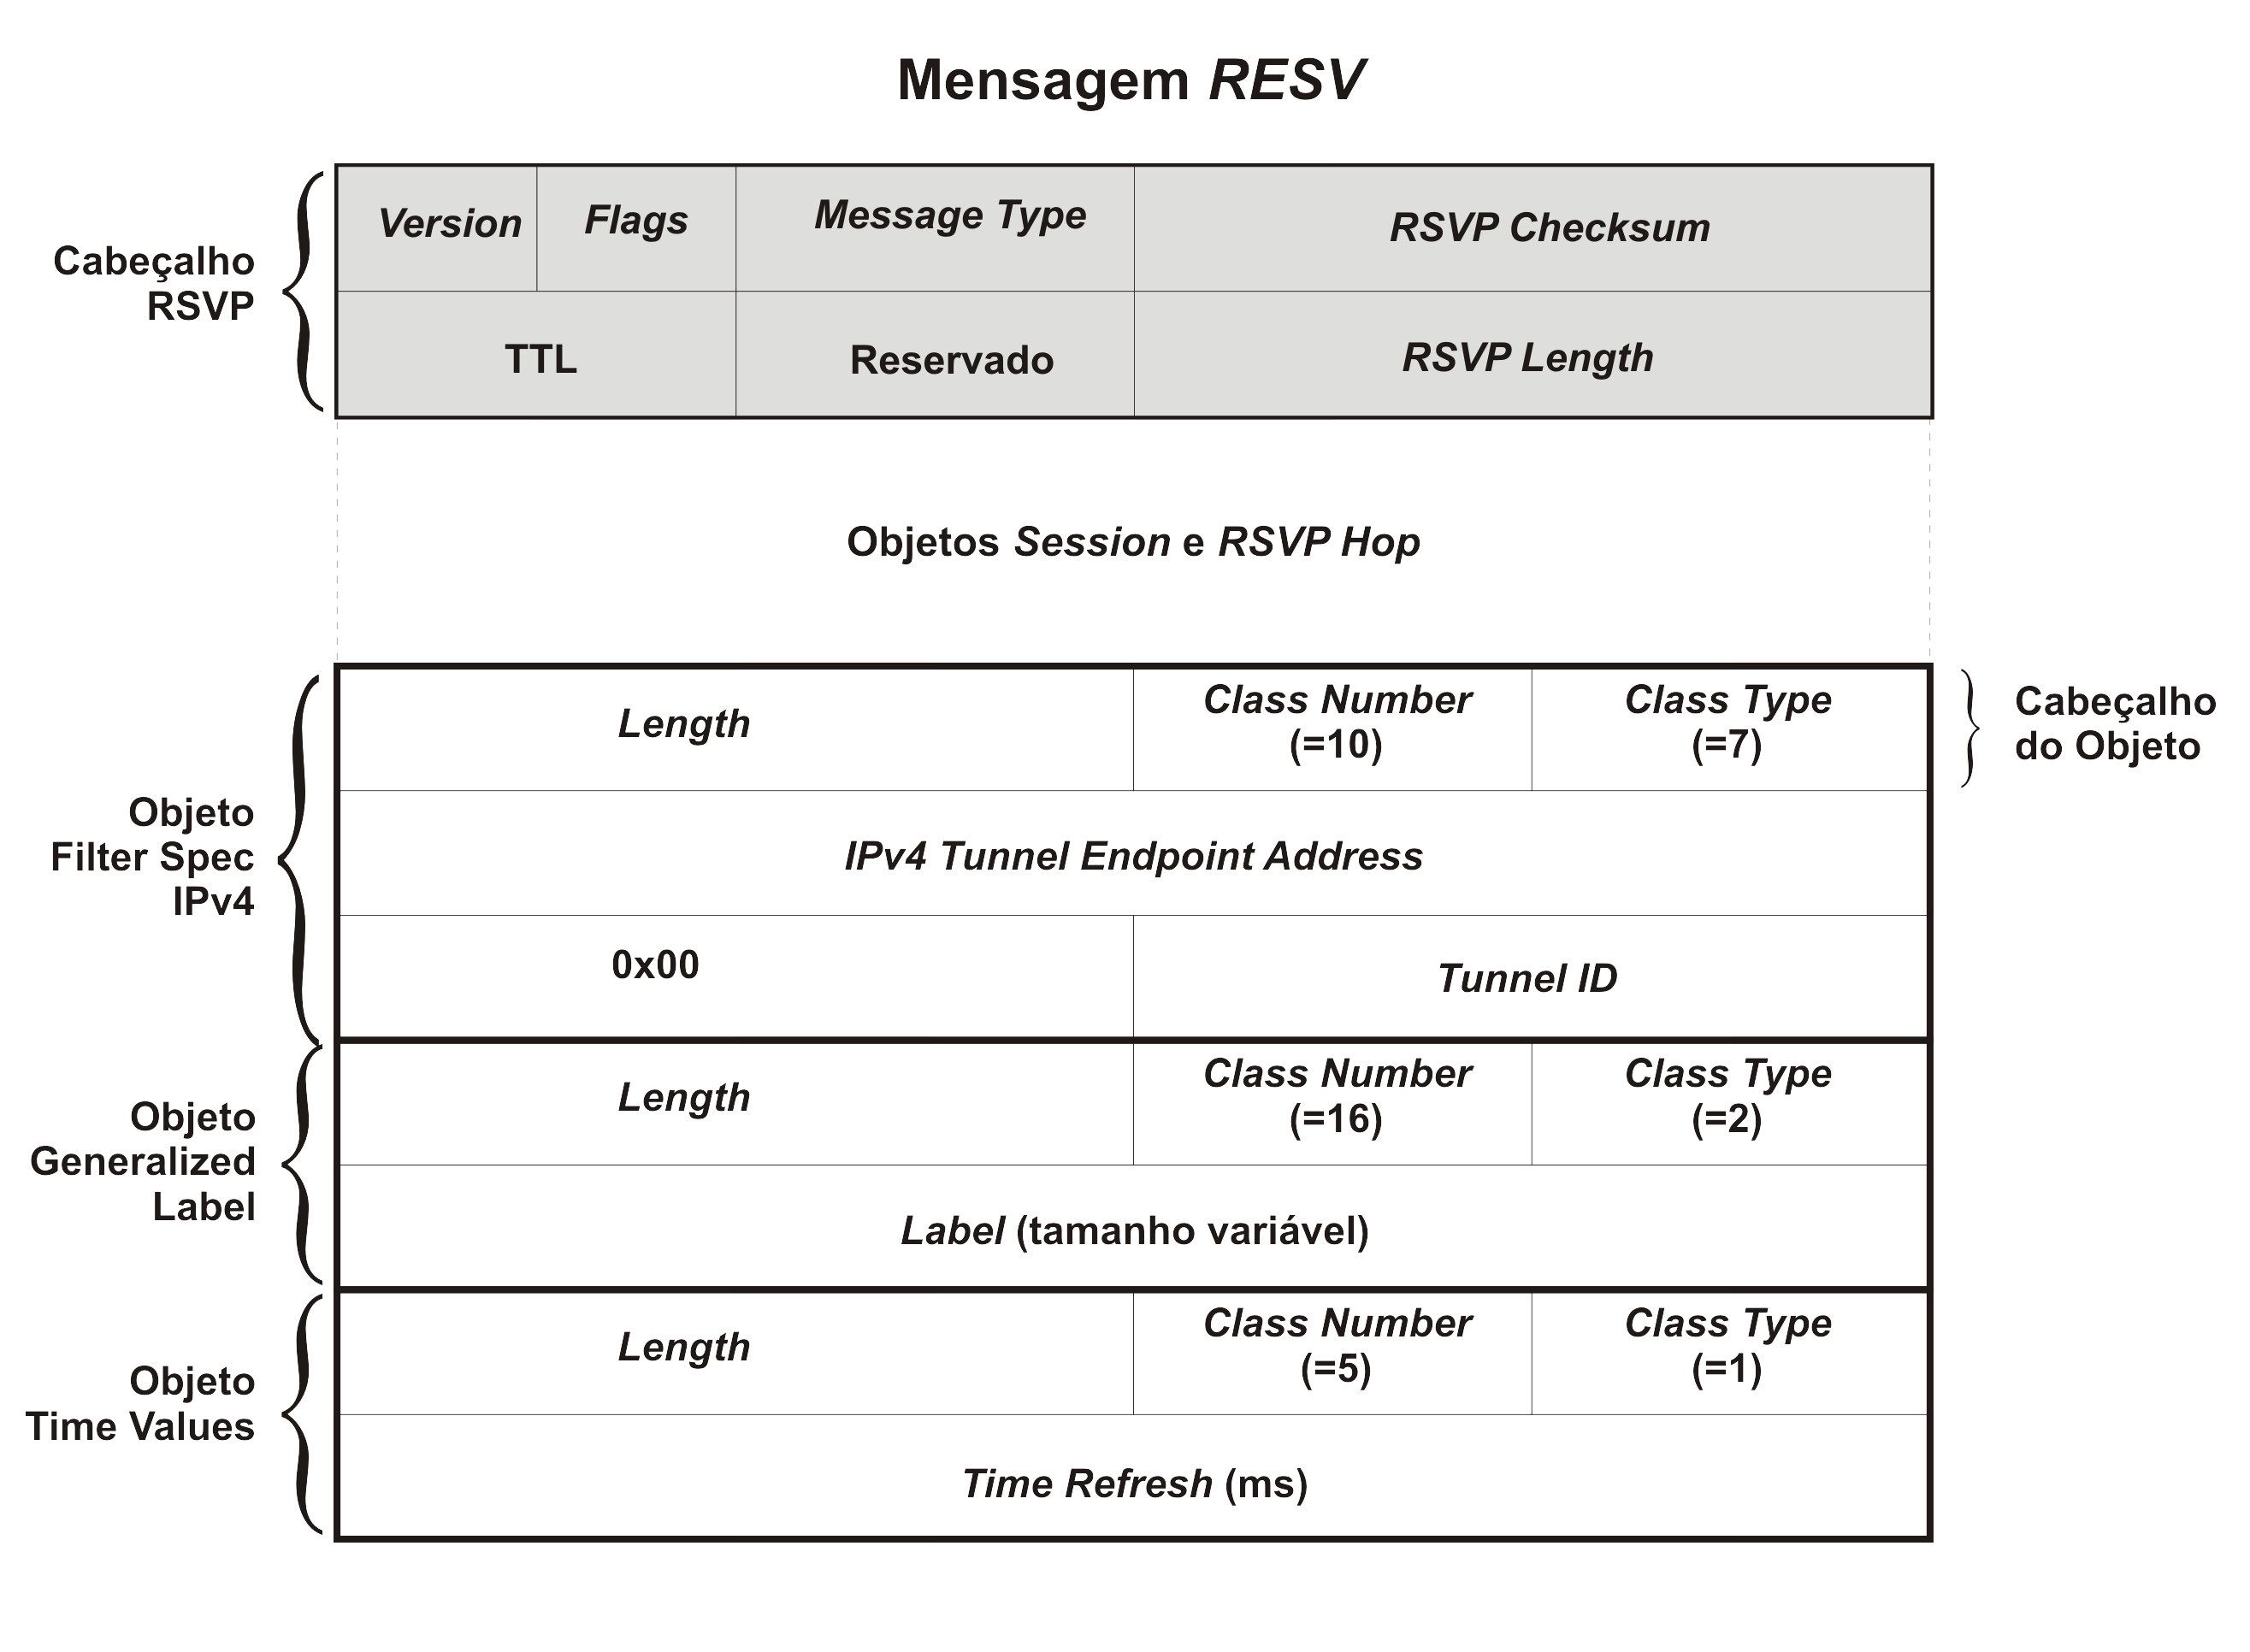
\includegraphics[scale=1]{cap4/rsvp-packet-resv.png}
	\caption{Estrutura da mensagem \textit{RESV} do protocolo RSVP-TE.}
	\label{fig:rsvppacketresv}
\end{figure}

\subsection{Manuten��o de LSPs}

O \ac{RSVP-TE} permite manter um estado de atividade flex�vel (\textit{soft-state}) das conex�es atrav�s troca de mensagens \textit{PATH} e \textit{RESV} de atualiza��o. A diferen�a entre as mensagens de atualiza��o e as de estabelecimento consiste na obrigatoriedade da mensagem de atualiza��o percorrer exatamente a mesma rota da mensagem \textit{PATH} original. Assim, para manter o caminho ativo, as novas mensagens \textit{PATH} devem transportar um objeto \textit{EXPLICIT ROUTE}, que cont�m todos os n�s da rota por onde a mensagem dever� ser transmitida. Se uma mensagem de atualiza��o n�o puder seguir por algum enlace do caminho devido a algum erro, uma nova rota � calculada somente contornando o local da falha. Logo, a mensagem deve seguir pelos n�s do caminho que n�o foram prejudicados. Se n�o for poss�vel restabelecer o \ac{LSP} utilizando o rerroteamento do local onde a falha ocorreu, mensagens \textit{PATHTEAR} e/ou \textit{RESVTEAR} ou mensagens de erro ser�o enviadas para remover o \ac{LSP}. Caso n�o seja poss�vel remover os estados armazenados nos n�s onde a falha ocorreu, os tempos de vida dos estados locais ir�o expirar, e consequentemente, ser�o removidos automaticamente. Este tipo de opera��o de interrup��o das atividades do caminho estabelecido e de tempo de vida finito dos estados do caminho em cada n� n�o � encontrado no mecanismo de estado de atividade fixo (\textit{hard-state}). Logo, para que um \textit{hard-state} \ac{LSP} seja rerroteado por outro caminho � necess�rio antes remov�-lo totalmente, para depois restabelec�-lo utilizando a nova rota. O \ac{CR-LDP}~\cite{rfc3472} � um exemplo de protocolo que faz uso do mecanismo \textit{hard-state}. Este protocolo tamb�m � suportado pelo \ac{GMPLS}.


\subsection{Remo��o de LSPs}

Um \ac{LSP} pode ser removido em duas situa��es: (\textit{i}) em fun��o do mecanismo \textit{soft-state} e (\textit{ii}) remo��o expl�cita por algum \ac{LSR} do caminho. A a��o natural de remo��o dever ser tomada pelo \ac{LSR} de ingresso, que envia uma mensagem \textit{PATHTEAR} propagando-se n�-a-n� at� o destino. A cada passo, o plano de controle local apaga os estados (\textit{PATHSTATE} e \textit{RESVSTATE}), depois ele encaminha a mensagem para o pr�ximo \textit{hop}.

Se a decis�o de remover o \c{LSP} for tomada pelo destino ou por um \ac{LSR} intermedi�rio, uma mensagem \textit{RESVTEAR} � enviada rumo � origem, que durante a sua propaga��o remove somente o \textit{RESVSTATE} dos n�s intermedi�rios.

\subsection{LSPs Bidirecionais}

A especifica��o do protocolo \ac{RSVP-TE} documentado sob a \ac{RFC} 3209~\cite{rfc3209} definiu um m�todo para o estabelecimento de \ac{LSP} bidirecionais. Neste caso, entretanto, era necess�ria a execu��o de duas trocas de sinaliza��o, uma para o sentido origem-destino (\textit{downstream}) e outra no sentido destino-origem (\textit{upstream}). Na \ac{RFC} 3473~\cite{rfc3473}, que define os requisitos do \ac{GMPLS} para o protocolo \ac{RSVP-TE}, a necessidade de sinaliza��o em sentidos opostos foi extinta, devido ao novo objeto \textit{UPSTREAM LABEL}.  Ent�o, para aprovisionar conex�es bidirecionais basta a origem enviar um r�tulo de \textit{upstream} em uma mensagem \textit{PATH} que contenha esse novo objeto. Logo, o r�tulo transmitido deve possui o mesmo formato do \textit{GENERALIZED LABEL} que ser� transportado pela \textit{RESV}. Assim o processo de estabelecimento de \acp{LSP} bidirecionais � simplificado. O exemplo ilustrado na Figura~\ref{fig:rsvppacketresv} tamb�m � v�lido para conex�es nos dois sentidos. Neste caso, o destino instala imediatamente o r�tulo de \textit{upstream} recebido na mensagem \textit{PATH}, que pode naquele instante come�ar a transmitir dados para a origem. 

\subsection{Mensagens de Erros}

No caso de erros durante a instala��o ou atividade de um \ac{LSP}, mensagens \textit{PATH ERROR} e \textit{RESV ERROR} s�o utilizadas para indicar o local das falhas e tamb�m o motivo de sua ocorr�ncia. A mensagem \textit{PATH ERROR} � enviada pelo destino ou por um n� intermedi�rio em dire��o � origem, mas s� poder� alterar os estados dos n�s intermedi�rios se uma \textit{flag} do objeto \textit{ERROR SPEC} estiver configurada com indicativo \textit{Path\_State\_Removed}~\cite{rfc3473}. Por outro lado, a mensagem \textit{RESV ERROR} propaga-se na dire��o do destino. Se necess�rio, ela poder� modificar o \textit{RESVSTATE} do n� intermedi�rio baseada no indicativo de erro transportado.

Quando duas mensagens \textit{RESV} est�o concorrendo pelo mesmo recurso de um enlace, poder� acontecer o erro chamado de conten��o, que significa que o recurso ser� alocado para uma das requisi��es, e consequentemente, a outra requisi��o ser� bloqueada. Neste caso, o local onde ocorreu o bloqueio dever� retornar mensagens \textit{PATH ERROR} e \textit{RESV ERROR} relativas � requisi��o bloqueada informando que o recurso n�o est� mais dispon�vel.


%\include{cap5/cap5a}
%\include{cap6/cap6a}
%\include{cap7/cap7a}

%\clearemptydoublepage
% Apendices
\appendix
%\include{app/app1}
%\include{app/app2}
%\include{app/app3}
\singlespacing
\chapter{Lista de Acr�nimos}

\begin{acronym}[RSVP-TE]
\acro{ADM}{\textit{Add/Drop Multiplexers}}
\acro{AGC}{\textit{Automatic Gain Control}}
\acro{ANSI}{\textit{American National Standards Institute}}
\acro{APC}{\textit{Automatic Power Control}}
\acro{APS-PCC}[APS/PCC]{\textit{Automatic Protection Switching/Protection Communication Channel}}
\acro{ASE}{\textit{Amplified Spontaneous Emission}}
\acro{ASON}{\textit{Automatically Switched Optical Network}}
\acro{ATM}{\textit{Asynchronous Transfer Mode}}
\acro{BDI}{\textit{Backward Deflect Indication} }
\acro{BEI}{\textit{Backward Error Indication}}
\acro{BER}{\textit{Bit Error Rate}}
\acro{BIAE}{\textit{Backward Incoming Alignment Error}}
\acro{BIP-8}{\textit{Bit Interleaved Parity-8}}
\acro{CCITT}{\textit{International Telegraph and Telephone Consultative Committee}}
\acro{CD}{\textit{Chromatic Dispersion}}
\acro{CBR}{\textit{Constant Bit Rate}}
\acro{CR-LDP}{\textit{Constraint-based Label Distribution Protocol}}
\acro{DCM}{\textit{Dispersion Compensation Module}}
\acro{DBPSK}{\textit{Differential Binary Phase Shift Keying}}
\acro{DPSK}{\textit{Differential Phase Shift Keying}}
\acro{ECSA}{\textit{Exchange Carriers Standards Association}}
\acro{EDFA}{\textit{Erbium Doped Fiber Amplifier}}
\acro{FC1200}{10 \textit{Gigabit Fibre Channel}}
\acro{FA}{\textit{Framing Alignment}}
\acro{FAS}{\textit{Framing Alignment Signal}}
\acro{FEC}{\textit{Forward Error Corrector}}
\acro{FSC}{\textit{Fiber Switch Capable}}
\acro{FSK}{\textit{Frequency-shift keying}}
\acro{FWM}{\textit{Four-Wave Mixing}}
\acro{FTFL}{\textit{Fault Type and Fault Location}}
\acro{GCC}{\textit{General Communication Channel}}
\acro{GFP}{\textit{Generic Framing Procedures}}
\acro{GMPLS}{\textit{Generalized Multi-Protocol Label Switching}}
\acro{IAE}{\textit{Incoming Alignment Error}}
\acro{IaDI}{\textit{Intra-domain interface}}
\acro{IANA}{\textit{Internet Assigned Numbers Authority}}
\acro{IA-RWA}{\textit{Impairment-Aware Routing and Wavelength Assingnment}}
\acro{IETF}{Internet Engineering Task Force}
\acro{IP}{\textit{Internet Protocol}}
\acro{IPv4}{\textit{Internet Protocol} vers�o 4}
\acro{IPv6}{\textit{Internet Protocol} vers�o 6}
\acro{IrDI}{\textit{Inter-domain interface}}
\acro{ITU-T}{\textit{International Telecommunication Union -- Telecommunication Standardization Sector}}
\acro{JC}{\textit{Justification Control}}
\acro{L2SC}{\textit{Layer 2 Switch Capable}}
\acro{LED}{\textit{Light-Emitting Diodes}}
\acro{LMP}{\textit{Link Management Protocol}}
\acro{LOF}{\textit{Loss Of Frame}}
\acro{LOM}{\textit{Loss Of Multiframe}}
\acro{LOS}{\textit{Loss Of Signal}}
%\acro{LSA}{Link-State Advertisement}
\acro{LSC}{\textit{Lambda Switch Capable}}
\acro{LSR}{\textit{Label Switch Router}}
\acro{LSP}{\textit{Label Switched Path}}
\acro{MFAS}{\textit{Multi-Frame Alignment Signal}}
\acro{MLM}{\textit{Multilongitudinal Mode Fabry-Perot Laser}}
\acro{MPLS}{\textit{Multi-Protocol Label Switching}}
\acro{MSOH}{\textit{Multiplex Section Overhead}}
\acro{NSFNet}{\textit{National Science Foundation Network}}
\acro{NTTNet}{\textit{Nippon Telegraph and Telephone Network}}
\acro{O-E-O}{�tica-Eletr�nica-�tica}
\acro{ROADM}{\textit{Reconfigurable Optical Add \slash~Drop Multiplexer}}
\acro{OADM}{\textit{Optical Add \slash~Drop Multiplexer}}
\acro{OAMP}[OAM\&P]{\textit{Operation, Administration, Maintenance and Provisioning}}
\acro{OCh}{\textit{Optical Channel}}
\acro{OChr}{\textit{Optical Channel With Reduced Functionality}}
\acro{ODU}{\textit{Optical Channel Data Unit}}
\acro{OLT}{\textit{Optical Line Terminator}}
\acro{OMS}{\textit{Optical Multiplex Section}}
\acro{OOF}{\textit{Out Of Frame}}
\acro{OOK}{\textit{On-off keying}}
\acro{OOM}{\textit{Out Of Multiframe}}
\acro{OPEX}{\textit{Operational Expenditure}}
\acro{OPS}{\textit{Optical Physical Section}}
\acro{OPU}{\textit{Optical Channel Payload Unit}}
\acro{OSPF-TE}{\textit{Open Shortest Path First with Traffic Engineering}}
\acro{OTH}{\textit{Optical Transport Hierarchy}}
\acro{OTN}{\textit{Optical Transport Network}}
\acro{OTS}{\textit{Optical Transmission Section}}
\acro{OTU}{\textit{Optical Channel Transport Unit}}
\acro{OH}{\textit{overhead}}
\acro{OXC}{\textit{Optical Cross-Connect}}
\acro{PDH}{\textit{Plesiochronous Digital Hierarchy}}
\acro{POH}{\textit{Path Overhead}}
\acro{POLSK}{\textit{Polarization-shift Keying}}
\acro{PM}{\textit{Path Monitoring}}
\acro{PMD}{\textit{Polarization Mode Dispersion}}
\acro{PSC}{\textit{Packet Switch Capable}}
\acro{PSI}{\textit{Payload structure identifier}}
\acro{PSK}{\textit{Phase-shift keying}}
\acro{PT}{\textit{Payload Type}}
\acro{Pin}[$P_{in}$]{\textit{Power input}}
\acro{Pout}[$P_{out}$]{\textit{Power output}}
\acro{QoS}{\textit{Quality of Service}}
\acro{QoT}{\textit{Quality of Transmission}}
\acro{REG}{Regenerador}
\acro{RFC}{\textit{Request For Comments}}
\acro{RS}{Reed-Solomon}
\acro{RSOH}{\textit{Regenerator Section Overhead}}
\acro{RSVP}{\textit{Resource ReSerVation Protocol}}
\acro{RSVP-TE}{\textit{Resource ReSerVation Protocol with Traffic Engineering}}
\acro{RWA}{\textit{Routing and Wavelength Assignment}}
%\acro{SI}{Swarm Intelligence}
\acro{SLM}{\textit{Single Longitudinal Mode Distributed-Feedback Laser}}
\acro{SM}{\textit{Section Monitoring}}
\acro{SNR}{\textit{Signal-Noise Ratio}}
\acro{SAN}{\textit{Storage Area Network}}
\acro{SBS}{\textit{Stimulated Brillouin Scattering}}
\acro{SONET}{\textit{Synchronous Optical Networking}}
\acro{SDH}{\textit{Synchronous Digital Hierarchy}}
%\acro{SP}{Shortest Path}
\acro{SOH}{\textit{Section Overhead}}
\acro{SPM}{\textit{Self-Phase Modulation}}
\acro{STM}{\textit{Synchronous Transport Module}}
%\acro{SRLG}{Shared Risk Link Group}
\acro{SRS}{\textit{Stimulated Raman Scattering}}
\acro{TCM}{\textit{Tandem Connection Monitoring}}
\acro{TCP}{Transmission Control Protocol}
\acro{TDM}{\textit{Time Division Multiplexing}}
\acro{TE}{\textit{Traffic Engineering}}
\acro{TM}{\textit{Terminal Multiplexers}}
\acro{TTI}{\textit{Trail Trace Identifier}}
\acro{TLV}{Type-Length-Value}
\acro{UFABC}{Universidade Federal do ABC}
\acro{UNICAMP}{Universidade Estadual de Campinas}
\acro{UDP}{\textit{User Datagram Protocol}}
\acro{USP}{Universidade de S�o Paulo}
\acro{VC}{\textit{Virtual Container}}
\acro{VCAT}{\textit{Virtual Concatenator}}
\acro{VoIP}{\textit{Voice over IP}}
\acro{WDM}{\textit{Wavelength Division Multiplexing}}
%\acro{WDS}{Wavelength and Delay Selection}
%\acro{WRN}{Wavelength Routing Node}
%\acro{WRON}{Wavelength Routed Optical Network}
%\acro{WRS}{Wavelength Routing Switch}
\acro{XPM}{\textit{Cross-Phase Modulation}}
\acro{SDN}{\textit{Software Defined Networking}}
\acro{IPTV}{\textit{Internet Protocol Television}}
\acro{STS}{\textit{Synchronous Transport Signal}}
\end{acronym}
% ----------------------------------------------------------------------
% Bibliografia
%author index
%\chapter{�ndice Remissivo de Autores}
%\begin{multicols}{2}
%\printauthorindex
%\end{multicols}
%\singlespacing
%\clearemptydoublepage
\addcontentsline{toc}{chapter}{\numberline{}Refer�ncias Bibliogr�ficas}
\bibliographystyle{IEEEtran}
\bibliography{artigos,referencias,rfc}
\end{document} 